\documentclass[twoside]{book}

% Packages required by doxygen
\usepackage{calc}
\usepackage{doxygen}
\usepackage{graphicx}
\usepackage[utf8]{inputenc}
\usepackage{makeidx}
\usepackage{multicol}
\usepackage{multirow}
\usepackage{fixltx2e}
\PassOptionsToPackage{warn}{textcomp}
\usepackage{textcomp}
\usepackage[nointegrals]{wasysym}
\usepackage[table]{xcolor}

% Font selection
\usepackage[T1]{fontenc}
\usepackage{mathptmx}
\usepackage[scaled=.90]{helvet}
\usepackage{courier}
\usepackage{amssymb}
\usepackage{sectsty}
\renewcommand{\familydefault}{\sfdefault}
\allsectionsfont{%
  \fontseries{bc}\selectfont%
  \color{darkgray}%
}
\renewcommand{\DoxyLabelFont}{%
  \fontseries{bc}\selectfont%
  \color{darkgray}%
}
\newcommand{\+}{\discretionary{\mbox{\scriptsize$\hookleftarrow$}}{}{}}

% Page & text layout
\usepackage{geometry}
\geometry{%
  a4paper,%
  top=2.5cm,%
  bottom=2.5cm,%
  left=2.5cm,%
  right=2.5cm%
}
\tolerance=750
\hfuzz=15pt
\hbadness=750
\setlength{\emergencystretch}{15pt}
\setlength{\parindent}{0cm}
\setlength{\parskip}{0.2cm}
\makeatletter
\renewcommand{\paragraph}{%
  \@startsection{paragraph}{4}{0ex}{-1.0ex}{1.0ex}{%
    \normalfont\normalsize\bfseries\SS@parafont%
  }%
}
\renewcommand{\subparagraph}{%
  \@startsection{subparagraph}{5}{0ex}{-1.0ex}{1.0ex}{%
    \normalfont\normalsize\bfseries\SS@subparafont%
  }%
}
\makeatother

% Headers & footers
\usepackage{fancyhdr}
\pagestyle{fancyplain}
\fancyhead[LE]{\fancyplain{}{\bfseries\thepage}}
\fancyhead[CE]{\fancyplain{}{}}
\fancyhead[RE]{\fancyplain{}{\bfseries\leftmark}}
\fancyhead[LO]{\fancyplain{}{\bfseries\rightmark}}
\fancyhead[CO]{\fancyplain{}{}}
\fancyhead[RO]{\fancyplain{}{\bfseries\thepage}}
\fancyfoot[LE]{\fancyplain{}{}}
\fancyfoot[CE]{\fancyplain{}{}}
\fancyfoot[RE]{\fancyplain{}{\bfseries\scriptsize Generated on Thu May 1 2014 19\+:15\+:00 for My Project by Doxygen }}
\fancyfoot[LO]{\fancyplain{}{\bfseries\scriptsize Generated on Thu May 1 2014 19\+:15\+:00 for My Project by Doxygen }}
\fancyfoot[CO]{\fancyplain{}{}}
\fancyfoot[RO]{\fancyplain{}{}}
\renewcommand{\footrulewidth}{0.4pt}
\renewcommand{\chaptermark}[1]{%
  \markboth{#1}{}%
}
\renewcommand{\sectionmark}[1]{%
  \markright{\thesection\ #1}%
}

% Indices & bibliography
\usepackage{natbib}
\usepackage[titles]{tocloft}
\setcounter{tocdepth}{3}
\setcounter{secnumdepth}{5}
\makeindex

% Hyperlinks (required, but should be loaded last)
\usepackage{ifpdf}
\ifpdf
  \usepackage[pdftex,pagebackref=true]{hyperref}
\else
  \usepackage[ps2pdf,pagebackref=true]{hyperref}
\fi
\hypersetup{%
  colorlinks=true,%
  linkcolor=blue,%
  citecolor=blue,%
  unicode%
}

% Custom commands
\newcommand{\clearemptydoublepage}{%
  \newpage{\pagestyle{empty}\cleardoublepage}%
}


%===== C O N T E N T S =====

\begin{document}

% Titlepage & ToC
\hypersetup{pageanchor=false,
             bookmarks=true,
             bookmarksnumbered=true,
             pdfencoding=unicode
            }
\pagenumbering{roman}
\begin{titlepage}
\vspace*{7cm}
\begin{center}%
{\Large My Project }\\
\vspace*{1cm}
{\large Generated by Doxygen 1.8.7}\\
\vspace*{0.5cm}
{\small Thu May 1 2014 19:15:00}\\
\end{center}
\end{titlepage}
\clearemptydoublepage
\tableofcontents
\clearemptydoublepage
\pagenumbering{arabic}
\hypersetup{pageanchor=true}

%--- Begin generated contents ---
\chapter{Namespace Index}
\section{Namespace List}
Here is a list of all documented namespaces with brief descriptions\+:\begin{DoxyCompactList}
\item\contentsline{section}{\hyperlink{namespaceread__input}{read\+\_\+input} }{\pageref{namespaceread__input}}{}
\end{DoxyCompactList}

\chapter{Hierarchical Index}
\section{Class Hierarchy}
This inheritance list is sorted roughly, but not completely, alphabetically\+:\begin{DoxyCompactList}
\item \contentsline{section}{Molecule.\+Molecule}{\pageref{classMolecule_1_1Molecule}}{}
\item object\begin{DoxyCompactList}
\item \contentsline{section}{element.\+Element}{\pageref{classelement_1_1Element}}{}
\item \contentsline{section}{element.\+Elements\+Dict}{\pageref{classelement_1_1ElementsDict}}{}
\item \contentsline{section}{element.\+Isotope}{\pageref{classelement_1_1Isotope}}{}
\item \contentsline{section}{element.\+lazyattr}{\pageref{classelement_1_1lazyattr}}{}
\end{DoxyCompactList}
\item \contentsline{section}{Propertyclasses.\+Polarizability}{\pageref{classPropertyclasses_1_1Polarizability}}{}
\item \contentsline{section}{Property.\+Property}{\pageref{classProperty_1_1Property}}{}
\begin{DoxyCompactList}
\item \contentsline{section}{Propertyclasses.\+Property\+\_\+1\+\_\+\+Tensor}{\pageref{classPropertyclasses_1_1Property__1__Tensor}}{}
\item \contentsline{section}{Propertyclasses.\+Property\+\_\+2\+\_\+\+Tensor}{\pageref{classPropertyclasses_1_1Property__2__Tensor}}{}
\item \contentsline{section}{Propertyclasses.\+Property\+\_\+3\+\_\+\+Tensor}{\pageref{classPropertyclasses_1_1Property__3__Tensor}}{}
\end{DoxyCompactList}
\item Test\+Case\begin{DoxyCompactList}
\item \contentsline{section}{abavib\+\_\+unittester.\+abavib\+\_\+test}{\pageref{classabavib__unittester_1_1abavib__test}}{}
\begin{DoxyCompactList}
\item \contentsline{section}{abavib\+\_\+unittester.\+cubic\+\_\+force\+\_\+field\+\_\+test}{\pageref{classabavib__unittester_1_1cubic__force__field__test}}{}
\item \contentsline{section}{abavib\+\_\+unittester.\+dipole\+\_\+test}{\pageref{classabavib__unittester_1_1dipole__test}}{}
\item \contentsline{section}{abavib\+\_\+unittester.\+effective\+\_\+geometry\+\_\+test}{\pageref{classabavib__unittester_1_1effective__geometry__test}}{}
\item \contentsline{section}{abavib\+\_\+unittester.\+frequency\+\_\+test}{\pageref{classabavib__unittester_1_1frequency__test}}{}
\item \contentsline{section}{abavib\+\_\+unittester.\+g\+\_\+factor\+\_\+test}{\pageref{classabavib__unittester_1_1g__factor__test}}{}
\item \contentsline{section}{abavib\+\_\+unittester.\+magnetizability\+\_\+test}{\pageref{classabavib__unittester_1_1magnetizability__test}}{}
\item \contentsline{section}{abavib\+\_\+unittester.\+molecular\+\_\+quadrupole\+\_\+test}{\pageref{classabavib__unittester_1_1molecular__quadrupole__test}}{}
\item \contentsline{section}{abavib\+\_\+unittester.\+nuclear\+\_\+quadrupole\+\_\+test}{\pageref{classabavib__unittester_1_1nuclear__quadrupole__test}}{}
\item \contentsline{section}{abavib\+\_\+unittester.\+polarizability\+\_\+test}{\pageref{classabavib__unittester_1_1polarizability__test}}{}
\item \contentsline{section}{abavib\+\_\+unittester.\+read\+\_\+hessian\+\_\+test}{\pageref{classabavib__unittester_1_1read__hessian__test}}{}
\item \contentsline{section}{abavib\+\_\+unittester.\+read\+\_\+molecule\+\_\+test}{\pageref{classabavib__unittester_1_1read__molecule__test}}{}
\item \contentsline{section}{abavib\+\_\+unittester.\+shield\+\_\+test}{\pageref{classabavib__unittester_1_1shield__test}}{}
\item \contentsline{section}{abavib\+\_\+unittester.\+spin\+\_\+rotation\+\_\+constants\+\_\+test}{\pageref{classabavib__unittester_1_1spin__rotation__constants__test}}{}
\end{DoxyCompactList}
\item \contentsline{section}{chiral\+\_\+tester.\+abavib\+\_\+test}{\pageref{classchiral__tester_1_1abavib__test}}{}
\begin{DoxyCompactList}
\item \contentsline{section}{chiral\+\_\+tester.\+cubic\+\_\+force\+\_\+field\+\_\+test}{\pageref{classchiral__tester_1_1cubic__force__field__test}}{}
\item \contentsline{section}{chiral\+\_\+tester.\+frequency\+\_\+test}{\pageref{classchiral__tester_1_1frequency__test}}{}
\item \contentsline{section}{chiral\+\_\+tester.\+optical\+\_\+rotation\+\_\+test}{\pageref{classchiral__tester_1_1optical__rotation__test}}{}
\item \contentsline{section}{chiral\+\_\+tester.\+read\+\_\+hessian\+\_\+test}{\pageref{classchiral__tester_1_1read__hessian__test}}{}
\item \contentsline{section}{chiral\+\_\+tester.\+read\+\_\+molecule\+\_\+test}{\pageref{classchiral__tester_1_1read__molecule__test}}{}
\end{DoxyCompactList}
\end{DoxyCompactList}
\end{DoxyCompactList}

\chapter{Class Index}
\section{Class List}
Here are the classes, structs, unions and interfaces with brief descriptions\+:
\begin{DoxyCompactList}
\item\contentsline{section}{\hyperlink{classabavib__unittester_1_1abavib__test}{abavib\+\_\+unittester.\+abavib\+\_\+test} }{\pageref{classabavib__unittester_1_1abavib__test}}{}
\item\contentsline{section}{\hyperlink{classchiral__tester_1_1abavib__test}{chiral\+\_\+tester.\+abavib\+\_\+test} }{\pageref{classchiral__tester_1_1abavib__test}}{}
\item\contentsline{section}{\hyperlink{classabavib__unittester_1_1cubic__force__field__test}{abavib\+\_\+unittester.\+cubic\+\_\+force\+\_\+field\+\_\+test} }{\pageref{classabavib__unittester_1_1cubic__force__field__test}}{}
\item\contentsline{section}{\hyperlink{classchiral__tester_1_1cubic__force__field__test}{chiral\+\_\+tester.\+cubic\+\_\+force\+\_\+field\+\_\+test} }{\pageref{classchiral__tester_1_1cubic__force__field__test}}{}
\item\contentsline{section}{\hyperlink{classabavib__unittester_1_1dipole__test}{abavib\+\_\+unittester.\+dipole\+\_\+test} }{\pageref{classabavib__unittester_1_1dipole__test}}{}
\item\contentsline{section}{\hyperlink{classabavib__unittester_1_1effective__geometry__test}{abavib\+\_\+unittester.\+effective\+\_\+geometry\+\_\+test} }{\pageref{classabavib__unittester_1_1effective__geometry__test}}{}
\item\contentsline{section}{\hyperlink{classelement_1_1Element}{element.\+Element} }{\pageref{classelement_1_1Element}}{}
\item\contentsline{section}{\hyperlink{classelement_1_1ElementsDict}{element.\+Elements\+Dict} }{\pageref{classelement_1_1ElementsDict}}{}
\item\contentsline{section}{\hyperlink{classchiral__tester_1_1frequency__test}{chiral\+\_\+tester.\+frequency\+\_\+test} }{\pageref{classchiral__tester_1_1frequency__test}}{}
\item\contentsline{section}{\hyperlink{classabavib__unittester_1_1frequency__test}{abavib\+\_\+unittester.\+frequency\+\_\+test} }{\pageref{classabavib__unittester_1_1frequency__test}}{}
\item\contentsline{section}{\hyperlink{classabavib__unittester_1_1g__factor__test}{abavib\+\_\+unittester.\+g\+\_\+factor\+\_\+test} }{\pageref{classabavib__unittester_1_1g__factor__test}}{}
\item\contentsline{section}{\hyperlink{classelement_1_1Isotope}{element.\+Isotope} }{\pageref{classelement_1_1Isotope}}{}
\item\contentsline{section}{\hyperlink{classelement_1_1lazyattr}{element.\+lazyattr} }{\pageref{classelement_1_1lazyattr}}{}
\item\contentsline{section}{\hyperlink{classabavib__unittester_1_1magnetizability__test}{abavib\+\_\+unittester.\+magnetizability\+\_\+test} }{\pageref{classabavib__unittester_1_1magnetizability__test}}{}
\item\contentsline{section}{\hyperlink{classabavib__unittester_1_1molecular__quadrupole__test}{abavib\+\_\+unittester.\+molecular\+\_\+quadrupole\+\_\+test} }{\pageref{classabavib__unittester_1_1molecular__quadrupole__test}}{}
\item\contentsline{section}{\hyperlink{classMolecule_1_1Molecule}{Molecule.\+Molecule} }{\pageref{classMolecule_1_1Molecule}}{}
\item\contentsline{section}{\hyperlink{classabavib__unittester_1_1nuclear__quadrupole__test}{abavib\+\_\+unittester.\+nuclear\+\_\+quadrupole\+\_\+test} }{\pageref{classabavib__unittester_1_1nuclear__quadrupole__test}}{}
\item\contentsline{section}{\hyperlink{classchiral__tester_1_1optical__rotation__test}{chiral\+\_\+tester.\+optical\+\_\+rotation\+\_\+test} }{\pageref{classchiral__tester_1_1optical__rotation__test}}{}
\item\contentsline{section}{\hyperlink{classPropertyclasses_1_1Polarizability}{Propertyclasses.\+Polarizability} }{\pageref{classPropertyclasses_1_1Polarizability}}{}
\item\contentsline{section}{\hyperlink{classabavib__unittester_1_1polarizability__test}{abavib\+\_\+unittester.\+polarizability\+\_\+test} }{\pageref{classabavib__unittester_1_1polarizability__test}}{}
\item\contentsline{section}{\hyperlink{classProperty_1_1Property}{Property.\+Property} }{\pageref{classProperty_1_1Property}}{}
\item\contentsline{section}{\hyperlink{classPropertyclasses_1_1Property__1__Tensor}{Propertyclasses.\+Property\+\_\+1\+\_\+\+Tensor} }{\pageref{classPropertyclasses_1_1Property__1__Tensor}}{}
\item\contentsline{section}{\hyperlink{classPropertyclasses_1_1Property__2__Tensor}{Propertyclasses.\+Property\+\_\+2\+\_\+\+Tensor} }{\pageref{classPropertyclasses_1_1Property__2__Tensor}}{}
\item\contentsline{section}{\hyperlink{classPropertyclasses_1_1Property__3__Tensor}{Propertyclasses.\+Property\+\_\+3\+\_\+\+Tensor} }{\pageref{classPropertyclasses_1_1Property__3__Tensor}}{}
\item\contentsline{section}{\hyperlink{classchiral__tester_1_1read__hessian__test}{chiral\+\_\+tester.\+read\+\_\+hessian\+\_\+test} }{\pageref{classchiral__tester_1_1read__hessian__test}}{}
\item\contentsline{section}{\hyperlink{classabavib__unittester_1_1read__hessian__test}{abavib\+\_\+unittester.\+read\+\_\+hessian\+\_\+test} }{\pageref{classabavib__unittester_1_1read__hessian__test}}{}
\item\contentsline{section}{\hyperlink{classchiral__tester_1_1read__molecule__test}{chiral\+\_\+tester.\+read\+\_\+molecule\+\_\+test} }{\pageref{classchiral__tester_1_1read__molecule__test}}{}
\item\contentsline{section}{\hyperlink{classabavib__unittester_1_1read__molecule__test}{abavib\+\_\+unittester.\+read\+\_\+molecule\+\_\+test} }{\pageref{classabavib__unittester_1_1read__molecule__test}}{}
\item\contentsline{section}{\hyperlink{classabavib__unittester_1_1shield__test}{abavib\+\_\+unittester.\+shield\+\_\+test} }{\pageref{classabavib__unittester_1_1shield__test}}{}
\item\contentsline{section}{\hyperlink{classabavib__unittester_1_1spin__rotation__constants__test}{abavib\+\_\+unittester.\+spin\+\_\+rotation\+\_\+constants\+\_\+test} }{\pageref{classabavib__unittester_1_1spin__rotation__constants__test}}{}
\end{DoxyCompactList}

\chapter{Namespace Documentation}
\hypertarget{namespaceread__input}{\section{read\+\_\+input Namespace Reference}
\label{namespaceread__input}\index{read\+\_\+input@{read\+\_\+input}}
}
\subsection*{Functions}
\begin{DoxyCompactItemize}
\item 
def \hyperlink{namespaceread__input_a8044a25ca166989f90bc28ea72ed7272}{read\+\_\+molecule}
\item 
def \hyperlink{namespaceread__input_ad33b518c2d8d751c205afde02365170e}{read\+\_\+hessian}
\item 
def \hyperlink{namespaceread__input_ad0bb9762c4aec6cd6804ee183811d55f}{read\+\_\+\+M\+O\+L\+Q\+U\+A\+D}
\item 
def \hyperlink{namespaceread__input_adc81b827a0cc310a3d429d393bd4d906}{read\+\_\+\+M\+A\+G\+N\+E\+T}
\item 
def \hyperlink{namespaceread__input_a2bba32ea57a1240d218dfdaceda12421}{read\+\_\+\+G\+F\+A\+C\+T\+O\+R}
\item 
def \hyperlink{namespaceread__input_a926ccdb92fd82370dfa7bba7883d5f18}{read\+\_\+\+P\+O\+L\+A\+R\+I}
\item 
def \hyperlink{namespaceread__input_af7138756561f70b3f0cdf92cf10b393d}{read\+\_\+\+S\+P\+I\+N\+R\+O\+T}
\item 
def \hyperlink{namespaceread__input_a831683736d21bb282abb8ae538d32950}{read\+\_\+\+N\+U\+C\+Q\+U\+A\+D}
\item 
def \hyperlink{namespaceread__input_a485488cc474cf816525ac3151b0975e6}{read\+\_\+\+O\+P\+T\+R\+O\+T}
\item 
def \hyperlink{namespaceread__input_ae727944c5af5d8c1eb576fea2e5e9480}{read\+\_\+2d\+\_\+input}
\item 
def \hyperlink{namespaceread__input_a3ebeb29cc6755437e0c8efa7668cb5f6}{read\+\_\+\+S\+H\+I\+E\+L\+D}
\item 
def \hyperlink{namespaceread__input_a2596d0058939865f2888683a371e6183}{read\+\_\+quartic\+\_\+force\+\_\+field1}
\item 
def \hyperlink{namespaceread__input_aaa16fddd2ee6c7e9a7f8533c16867605}{read\+\_\+\+D\+A\+L\+T\+O\+N\+\_\+\+N\+U\+C\+Q\+U\+A\+D}
\item 
def \hyperlink{namespaceread__input_a1eff34334e7b57f70439c1c70d74723c}{read\+\_\+\+D\+A\+L\+T\+O\+N\+\_\+\+S\+H\+I\+E\+L\+D}
\item 
def \hyperlink{namespaceread__input_a8aac5eef6151620e5716d052619dcdb4}{read\+\_\+\+D\+A\+L\+T\+O\+N\+\_\+\+S\+P\+I\+N\+R\+O\+T}
\item 
def \hyperlink{namespaceread__input_a369e35f499980d6f1fcc4f124a51853f}{read\+\_\+\+D\+A\+L\+T\+O\+N\+\_\+\+M\+A\+G\+N\+E\+T}
\item 
def \hyperlink{namespaceread__input_a6d481af39bac4e74210d7642c28818f9}{read\+\_\+\+D\+A\+L\+T\+O\+N\+\_\+\+O\+P\+T\+R\+O\+T}
\item 
def \hyperlink{namespaceread__input_a4153675abaf286f3d11e512f94f34c09}{read\+\_\+\+D\+A\+L\+T\+O\+N\+\_\+\+M\+O\+L\+Q\+U\+A\+D}
\item 
def \hyperlink{namespaceread__input_a88426418b4a30aa753d100056caeafd8}{read\+\_\+\+D\+A\+L\+T\+O\+N\+\_\+\+G\+F\+A\+C\+T\+O\+R}
\item 
def \hyperlink{namespaceread__input_a72d36f819fad47c5bf4da371d5d6190b}{read\+\_\+\+D\+A\+L\+T\+O\+N\+\_\+values\+\_\+2d}
\item 
def \hyperlink{namespaceread__input_a22bdcbd1e0b1955aefb4d4293092c060}{read\+\_\+eigenvector}
\item 
def \hyperlink{namespaceread__input_a71ccfa788319e09d446f5db99175fe0c}{read\+\_\+cubic\+\_\+force\+\_\+field}
\item 
def \hyperlink{namespaceread__input_a322e6108f22b89d25da80c4cbe60272a}{read\+\_\+cubic\+\_\+force\+\_\+field\+\_\+norm}
\end{DoxyCompactItemize}


\subsection{Detailed Description}
\begin{DoxyVerb}Module for reading DALTON input  
The functions of this module is:
read_mol_quad(filename, nm)
read_magnet(filename, nm)
def read_polari(filename, nm)
def read_spinrot(filename, natom, nm)
read_nucquad(filename, natom, nm)
def read_nucquad(filename, natom, nm)
def read_optrot(filename, nm)
def read_2d_input(filename, nm)
def read_3d_input(filename, nm)
read_4d_input(filename, natom, nm)
read_quartic_force_field(filename, n_cord)
read_DALTON_values_4d_reduced
read_DALTON_values_4d_full
read_DALTON_values_3d_reduced(filename)
read_DALTON_values_3d_full(filename)
read_cubic_force_field(filename, n_cord)
read_cubic_force_field_chiral(filename, n_cord)
write_to_file(molecule, property_type, results, n_atom = None)
\end{DoxyVerb}
 

\subsection{Function Documentation}
\hypertarget{namespaceread__input_ae727944c5af5d8c1eb576fea2e5e9480}{\index{read\+\_\+input@{read\+\_\+input}!read\+\_\+2d\+\_\+input@{read\+\_\+2d\+\_\+input}}
\index{read\+\_\+2d\+\_\+input@{read\+\_\+2d\+\_\+input}!read\+\_\+input@{read\+\_\+input}}
\subsubsection[{read\+\_\+2d\+\_\+input}]{\setlength{\rightskip}{0pt plus 5cm}def read\+\_\+input.\+read\+\_\+2d\+\_\+input (
\begin{DoxyParamCaption}
\item[{}]{filename, }
\item[{}]{nm}
\end{DoxyParamCaption}
)}}\label{namespaceread__input_ae727944c5af5d8c1eb576fea2e5e9480}
\begin{DoxyVerb}Reads and returns the second derivative of the property\end{DoxyVerb}
 \hypertarget{namespaceread__input_a71ccfa788319e09d446f5db99175fe0c}{\index{read\+\_\+input@{read\+\_\+input}!read\+\_\+cubic\+\_\+force\+\_\+field@{read\+\_\+cubic\+\_\+force\+\_\+field}}
\index{read\+\_\+cubic\+\_\+force\+\_\+field@{read\+\_\+cubic\+\_\+force\+\_\+field}!read\+\_\+input@{read\+\_\+input}}
\subsubsection[{read\+\_\+cubic\+\_\+force\+\_\+field}]{\setlength{\rightskip}{0pt plus 5cm}def read\+\_\+input.\+read\+\_\+cubic\+\_\+force\+\_\+field (
\begin{DoxyParamCaption}
\item[{}]{filename, }
\item[{}]{n\+\_\+cord}
\end{DoxyParamCaption}
)}}\label{namespaceread__input_a71ccfa788319e09d446f5db99175fe0c}
\begin{DoxyVerb}Reads and returns the cubic force field in cartessian coordinates
as a 4 dimensional np.array\end{DoxyVerb}
 \hypertarget{namespaceread__input_a322e6108f22b89d25da80c4cbe60272a}{\index{read\+\_\+input@{read\+\_\+input}!read\+\_\+cubic\+\_\+force\+\_\+field\+\_\+norm@{read\+\_\+cubic\+\_\+force\+\_\+field\+\_\+norm}}
\index{read\+\_\+cubic\+\_\+force\+\_\+field\+\_\+norm@{read\+\_\+cubic\+\_\+force\+\_\+field\+\_\+norm}!read\+\_\+input@{read\+\_\+input}}
\subsubsection[{read\+\_\+cubic\+\_\+force\+\_\+field\+\_\+norm}]{\setlength{\rightskip}{0pt plus 5cm}def read\+\_\+input.\+read\+\_\+cubic\+\_\+force\+\_\+field\+\_\+norm (
\begin{DoxyParamCaption}
\item[{}]{filename, }
\item[{}]{n\+\_\+nm}
\end{DoxyParamCaption}
)}}\label{namespaceread__input_a322e6108f22b89d25da80c4cbe60272a}
\begin{DoxyVerb}For testing purposes, extracts the correct values from DALTON\end{DoxyVerb}
 \hypertarget{namespaceread__input_a88426418b4a30aa753d100056caeafd8}{\index{read\+\_\+input@{read\+\_\+input}!read\+\_\+\+D\+A\+L\+T\+O\+N\+\_\+\+G\+F\+A\+C\+T\+O\+R@{read\+\_\+\+D\+A\+L\+T\+O\+N\+\_\+\+G\+F\+A\+C\+T\+O\+R}}
\index{read\+\_\+\+D\+A\+L\+T\+O\+N\+\_\+\+G\+F\+A\+C\+T\+O\+R@{read\+\_\+\+D\+A\+L\+T\+O\+N\+\_\+\+G\+F\+A\+C\+T\+O\+R}!read\+\_\+input@{read\+\_\+input}}
\subsubsection[{read\+\_\+\+D\+A\+L\+T\+O\+N\+\_\+\+G\+F\+A\+C\+T\+O\+R}]{\setlength{\rightskip}{0pt plus 5cm}def read\+\_\+input.\+read\+\_\+\+D\+A\+L\+T\+O\+N\+\_\+\+G\+F\+A\+C\+T\+O\+R (
\begin{DoxyParamCaption}
\item[{}]{filename}
\end{DoxyParamCaption}
)}}\label{namespaceread__input_a88426418b4a30aa753d100056caeafd8}
\begin{DoxyVerb}For testing purposes, extracts the correct values from DALTON\end{DoxyVerb}
 \hypertarget{namespaceread__input_a369e35f499980d6f1fcc4f124a51853f}{\index{read\+\_\+input@{read\+\_\+input}!read\+\_\+\+D\+A\+L\+T\+O\+N\+\_\+\+M\+A\+G\+N\+E\+T@{read\+\_\+\+D\+A\+L\+T\+O\+N\+\_\+\+M\+A\+G\+N\+E\+T}}
\index{read\+\_\+\+D\+A\+L\+T\+O\+N\+\_\+\+M\+A\+G\+N\+E\+T@{read\+\_\+\+D\+A\+L\+T\+O\+N\+\_\+\+M\+A\+G\+N\+E\+T}!read\+\_\+input@{read\+\_\+input}}
\subsubsection[{read\+\_\+\+D\+A\+L\+T\+O\+N\+\_\+\+M\+A\+G\+N\+E\+T}]{\setlength{\rightskip}{0pt plus 5cm}def read\+\_\+input.\+read\+\_\+\+D\+A\+L\+T\+O\+N\+\_\+\+M\+A\+G\+N\+E\+T (
\begin{DoxyParamCaption}
\item[{}]{filename}
\end{DoxyParamCaption}
)}}\label{namespaceread__input_a369e35f499980d6f1fcc4f124a51853f}
\begin{DoxyVerb}For testing purposes, extracts the correct values from DALTON\end{DoxyVerb}
 \hypertarget{namespaceread__input_a4153675abaf286f3d11e512f94f34c09}{\index{read\+\_\+input@{read\+\_\+input}!read\+\_\+\+D\+A\+L\+T\+O\+N\+\_\+\+M\+O\+L\+Q\+U\+A\+D@{read\+\_\+\+D\+A\+L\+T\+O\+N\+\_\+\+M\+O\+L\+Q\+U\+A\+D}}
\index{read\+\_\+\+D\+A\+L\+T\+O\+N\+\_\+\+M\+O\+L\+Q\+U\+A\+D@{read\+\_\+\+D\+A\+L\+T\+O\+N\+\_\+\+M\+O\+L\+Q\+U\+A\+D}!read\+\_\+input@{read\+\_\+input}}
\subsubsection[{read\+\_\+\+D\+A\+L\+T\+O\+N\+\_\+\+M\+O\+L\+Q\+U\+A\+D}]{\setlength{\rightskip}{0pt plus 5cm}def read\+\_\+input.\+read\+\_\+\+D\+A\+L\+T\+O\+N\+\_\+\+M\+O\+L\+Q\+U\+A\+D (
\begin{DoxyParamCaption}
\item[{}]{filename}
\end{DoxyParamCaption}
)}}\label{namespaceread__input_a4153675abaf286f3d11e512f94f34c09}
\begin{DoxyVerb}For testing purposes, extracts the correct values from DALTON\end{DoxyVerb}
 \hypertarget{namespaceread__input_aaa16fddd2ee6c7e9a7f8533c16867605}{\index{read\+\_\+input@{read\+\_\+input}!read\+\_\+\+D\+A\+L\+T\+O\+N\+\_\+\+N\+U\+C\+Q\+U\+A\+D@{read\+\_\+\+D\+A\+L\+T\+O\+N\+\_\+\+N\+U\+C\+Q\+U\+A\+D}}
\index{read\+\_\+\+D\+A\+L\+T\+O\+N\+\_\+\+N\+U\+C\+Q\+U\+A\+D@{read\+\_\+\+D\+A\+L\+T\+O\+N\+\_\+\+N\+U\+C\+Q\+U\+A\+D}!read\+\_\+input@{read\+\_\+input}}
\subsubsection[{read\+\_\+\+D\+A\+L\+T\+O\+N\+\_\+\+N\+U\+C\+Q\+U\+A\+D}]{\setlength{\rightskip}{0pt plus 5cm}def read\+\_\+input.\+read\+\_\+\+D\+A\+L\+T\+O\+N\+\_\+\+N\+U\+C\+Q\+U\+A\+D (
\begin{DoxyParamCaption}
\item[{}]{filename, }
\item[{}]{natom}
\end{DoxyParamCaption}
)}}\label{namespaceread__input_aaa16fddd2ee6c7e9a7f8533c16867605}
\begin{DoxyVerb}For testing purposes, extracts the correct values from DALTON\end{DoxyVerb}
 \hypertarget{namespaceread__input_a6d481af39bac4e74210d7642c28818f9}{\index{read\+\_\+input@{read\+\_\+input}!read\+\_\+\+D\+A\+L\+T\+O\+N\+\_\+\+O\+P\+T\+R\+O\+T@{read\+\_\+\+D\+A\+L\+T\+O\+N\+\_\+\+O\+P\+T\+R\+O\+T}}
\index{read\+\_\+\+D\+A\+L\+T\+O\+N\+\_\+\+O\+P\+T\+R\+O\+T@{read\+\_\+\+D\+A\+L\+T\+O\+N\+\_\+\+O\+P\+T\+R\+O\+T}!read\+\_\+input@{read\+\_\+input}}
\subsubsection[{read\+\_\+\+D\+A\+L\+T\+O\+N\+\_\+\+O\+P\+T\+R\+O\+T}]{\setlength{\rightskip}{0pt plus 5cm}def read\+\_\+input.\+read\+\_\+\+D\+A\+L\+T\+O\+N\+\_\+\+O\+P\+T\+R\+O\+T (
\begin{DoxyParamCaption}
\item[{}]{filename}
\end{DoxyParamCaption}
)}}\label{namespaceread__input_a6d481af39bac4e74210d7642c28818f9}
\begin{DoxyVerb}For testing purposes, extracts the correct values from DALTON\end{DoxyVerb}
 \hypertarget{namespaceread__input_a1eff34334e7b57f70439c1c70d74723c}{\index{read\+\_\+input@{read\+\_\+input}!read\+\_\+\+D\+A\+L\+T\+O\+N\+\_\+\+S\+H\+I\+E\+L\+D@{read\+\_\+\+D\+A\+L\+T\+O\+N\+\_\+\+S\+H\+I\+E\+L\+D}}
\index{read\+\_\+\+D\+A\+L\+T\+O\+N\+\_\+\+S\+H\+I\+E\+L\+D@{read\+\_\+\+D\+A\+L\+T\+O\+N\+\_\+\+S\+H\+I\+E\+L\+D}!read\+\_\+input@{read\+\_\+input}}
\subsubsection[{read\+\_\+\+D\+A\+L\+T\+O\+N\+\_\+\+S\+H\+I\+E\+L\+D}]{\setlength{\rightskip}{0pt plus 5cm}def read\+\_\+input.\+read\+\_\+\+D\+A\+L\+T\+O\+N\+\_\+\+S\+H\+I\+E\+L\+D (
\begin{DoxyParamCaption}
\item[{}]{filename, }
\item[{}]{natom}
\end{DoxyParamCaption}
)}}\label{namespaceread__input_a1eff34334e7b57f70439c1c70d74723c}
\begin{DoxyVerb}For testing purposes, extracts the correct values from DALTON\end{DoxyVerb}
 \hypertarget{namespaceread__input_a8aac5eef6151620e5716d052619dcdb4}{\index{read\+\_\+input@{read\+\_\+input}!read\+\_\+\+D\+A\+L\+T\+O\+N\+\_\+\+S\+P\+I\+N\+R\+O\+T@{read\+\_\+\+D\+A\+L\+T\+O\+N\+\_\+\+S\+P\+I\+N\+R\+O\+T}}
\index{read\+\_\+\+D\+A\+L\+T\+O\+N\+\_\+\+S\+P\+I\+N\+R\+O\+T@{read\+\_\+\+D\+A\+L\+T\+O\+N\+\_\+\+S\+P\+I\+N\+R\+O\+T}!read\+\_\+input@{read\+\_\+input}}
\subsubsection[{read\+\_\+\+D\+A\+L\+T\+O\+N\+\_\+\+S\+P\+I\+N\+R\+O\+T}]{\setlength{\rightskip}{0pt plus 5cm}def read\+\_\+input.\+read\+\_\+\+D\+A\+L\+T\+O\+N\+\_\+\+S\+P\+I\+N\+R\+O\+T (
\begin{DoxyParamCaption}
\item[{}]{filename, }
\item[{}]{natom}
\end{DoxyParamCaption}
)}}\label{namespaceread__input_a8aac5eef6151620e5716d052619dcdb4}
\begin{DoxyVerb}For testing purposes, extracts the correct values from DALTON\end{DoxyVerb}
 \hypertarget{namespaceread__input_a72d36f819fad47c5bf4da371d5d6190b}{\index{read\+\_\+input@{read\+\_\+input}!read\+\_\+\+D\+A\+L\+T\+O\+N\+\_\+values\+\_\+2d@{read\+\_\+\+D\+A\+L\+T\+O\+N\+\_\+values\+\_\+2d}}
\index{read\+\_\+\+D\+A\+L\+T\+O\+N\+\_\+values\+\_\+2d@{read\+\_\+\+D\+A\+L\+T\+O\+N\+\_\+values\+\_\+2d}!read\+\_\+input@{read\+\_\+input}}
\subsubsection[{read\+\_\+\+D\+A\+L\+T\+O\+N\+\_\+values\+\_\+2d}]{\setlength{\rightskip}{0pt plus 5cm}def read\+\_\+input.\+read\+\_\+\+D\+A\+L\+T\+O\+N\+\_\+values\+\_\+2d (
\begin{DoxyParamCaption}
\item[{}]{filename}
\end{DoxyParamCaption}
)}}\label{namespaceread__input_a72d36f819fad47c5bf4da371d5d6190b}
\begin{DoxyVerb}For testing purposes, extracts the correct values from DALTON\end{DoxyVerb}
 \hypertarget{namespaceread__input_a22bdcbd1e0b1955aefb4d4293092c060}{\index{read\+\_\+input@{read\+\_\+input}!read\+\_\+eigenvector@{read\+\_\+eigenvector}}
\index{read\+\_\+eigenvector@{read\+\_\+eigenvector}!read\+\_\+input@{read\+\_\+input}}
\subsubsection[{read\+\_\+eigenvector}]{\setlength{\rightskip}{0pt plus 5cm}def read\+\_\+input.\+read\+\_\+eigenvector (
\begin{DoxyParamCaption}
\item[{}]{filename, }
\item[{}]{n\+\_\+atoms}
\end{DoxyParamCaption}
)}}\label{namespaceread__input_a22bdcbd1e0b1955aefb4d4293092c060}
\begin{DoxyVerb}For testing purposes, extracts the correct values from DALTON\end{DoxyVerb}
 \hypertarget{namespaceread__input_a2bba32ea57a1240d218dfdaceda12421}{\index{read\+\_\+input@{read\+\_\+input}!read\+\_\+\+G\+F\+A\+C\+T\+O\+R@{read\+\_\+\+G\+F\+A\+C\+T\+O\+R}}
\index{read\+\_\+\+G\+F\+A\+C\+T\+O\+R@{read\+\_\+\+G\+F\+A\+C\+T\+O\+R}!read\+\_\+input@{read\+\_\+input}}
\subsubsection[{read\+\_\+\+G\+F\+A\+C\+T\+O\+R}]{\setlength{\rightskip}{0pt plus 5cm}def read\+\_\+input.\+read\+\_\+\+G\+F\+A\+C\+T\+O\+R (
\begin{DoxyParamCaption}
\item[{}]{filename, }
\item[{}]{nm}
\end{DoxyParamCaption}
)}}\label{namespaceread__input_a2bba32ea57a1240d218dfdaceda12421}
\begin{DoxyVerb}Reads and returns the second derivative of the property\end{DoxyVerb}
 \hypertarget{namespaceread__input_ad33b518c2d8d751c205afde02365170e}{\index{read\+\_\+input@{read\+\_\+input}!read\+\_\+hessian@{read\+\_\+hessian}}
\index{read\+\_\+hessian@{read\+\_\+hessian}!read\+\_\+input@{read\+\_\+input}}
\subsubsection[{read\+\_\+hessian}]{\setlength{\rightskip}{0pt plus 5cm}def read\+\_\+input.\+read\+\_\+hessian (
\begin{DoxyParamCaption}
\item[{}]{filename, }
\item[{}]{n\+\_\+coords}
\end{DoxyParamCaption}
)}}\label{namespaceread__input_ad33b518c2d8d751c205afde02365170e}
\begin{DoxyVerb}Reads a hessian from file.

filename: The name of the file the hessian is contained in. 
n_coords: The number of cartessian coordinates needed to express
          the location of the molecule ie. 3 * number of atoms 
return: A 2-dimensional np.array containg the hessian
\end{DoxyVerb}
 \hypertarget{namespaceread__input_adc81b827a0cc310a3d429d393bd4d906}{\index{read\+\_\+input@{read\+\_\+input}!read\+\_\+\+M\+A\+G\+N\+E\+T@{read\+\_\+\+M\+A\+G\+N\+E\+T}}
\index{read\+\_\+\+M\+A\+G\+N\+E\+T@{read\+\_\+\+M\+A\+G\+N\+E\+T}!read\+\_\+input@{read\+\_\+input}}
\subsubsection[{read\+\_\+\+M\+A\+G\+N\+E\+T}]{\setlength{\rightskip}{0pt plus 5cm}def read\+\_\+input.\+read\+\_\+\+M\+A\+G\+N\+E\+T (
\begin{DoxyParamCaption}
\item[{}]{filename, }
\item[{}]{nm}
\end{DoxyParamCaption}
)}}\label{namespaceread__input_adc81b827a0cc310a3d429d393bd4d906}
\begin{DoxyVerb}Reads and returns the second derivative of the property\end{DoxyVerb}
 \hypertarget{namespaceread__input_a8044a25ca166989f90bc28ea72ed7272}{\index{read\+\_\+input@{read\+\_\+input}!read\+\_\+molecule@{read\+\_\+molecule}}
\index{read\+\_\+molecule@{read\+\_\+molecule}!read\+\_\+input@{read\+\_\+input}}
\subsubsection[{read\+\_\+molecule}]{\setlength{\rightskip}{0pt plus 5cm}def read\+\_\+input.\+read\+\_\+molecule (
\begin{DoxyParamCaption}
\item[{}]{filename}
\end{DoxyParamCaption}
)}}\label{namespaceread__input_a8044a25ca166989f90bc28ea72ed7272}
\begin{DoxyVerb}Reads the MOLECULE.INP file generated be DALTON, and extracts the 
information we need from it.

filename: The name of the MOLECULE.INP file as saved in the input
          directory
return: The cartessian coordinates of the molecule as a list
        The masses of the atoms as a list
        The number of atoms as a list
        The charge of the atoms as a list
        The number of atoms in the molecule as an int
        The atoms making up the molecule as a list
\end{DoxyVerb}
 \hypertarget{namespaceread__input_ad0bb9762c4aec6cd6804ee183811d55f}{\index{read\+\_\+input@{read\+\_\+input}!read\+\_\+\+M\+O\+L\+Q\+U\+A\+D@{read\+\_\+\+M\+O\+L\+Q\+U\+A\+D}}
\index{read\+\_\+\+M\+O\+L\+Q\+U\+A\+D@{read\+\_\+\+M\+O\+L\+Q\+U\+A\+D}!read\+\_\+input@{read\+\_\+input}}
\subsubsection[{read\+\_\+\+M\+O\+L\+Q\+U\+A\+D}]{\setlength{\rightskip}{0pt plus 5cm}def read\+\_\+input.\+read\+\_\+\+M\+O\+L\+Q\+U\+A\+D (
\begin{DoxyParamCaption}
\item[{}]{filename, }
\item[{}]{nm}
\end{DoxyParamCaption}
)}}\label{namespaceread__input_ad0bb9762c4aec6cd6804ee183811d55f}
\begin{DoxyVerb}Reads and returns the second derivative of the property\end{DoxyVerb}
 \hypertarget{namespaceread__input_a831683736d21bb282abb8ae538d32950}{\index{read\+\_\+input@{read\+\_\+input}!read\+\_\+\+N\+U\+C\+Q\+U\+A\+D@{read\+\_\+\+N\+U\+C\+Q\+U\+A\+D}}
\index{read\+\_\+\+N\+U\+C\+Q\+U\+A\+D@{read\+\_\+\+N\+U\+C\+Q\+U\+A\+D}!read\+\_\+input@{read\+\_\+input}}
\subsubsection[{read\+\_\+\+N\+U\+C\+Q\+U\+A\+D}]{\setlength{\rightskip}{0pt plus 5cm}def read\+\_\+input.\+read\+\_\+\+N\+U\+C\+Q\+U\+A\+D (
\begin{DoxyParamCaption}
\item[{}]{filename, }
\item[{}]{natom, }
\item[{}]{nm}
\end{DoxyParamCaption}
)}}\label{namespaceread__input_a831683736d21bb282abb8ae538d32950}
\begin{DoxyVerb}Reads and returns the second derivative of the property\end{DoxyVerb}
\begin{DoxyVerb}Imports things needed from the DALTON.OUT that I need\end{DoxyVerb}
 \hypertarget{namespaceread__input_a485488cc474cf816525ac3151b0975e6}{\index{read\+\_\+input@{read\+\_\+input}!read\+\_\+\+O\+P\+T\+R\+O\+T@{read\+\_\+\+O\+P\+T\+R\+O\+T}}
\index{read\+\_\+\+O\+P\+T\+R\+O\+T@{read\+\_\+\+O\+P\+T\+R\+O\+T}!read\+\_\+input@{read\+\_\+input}}
\subsubsection[{read\+\_\+\+O\+P\+T\+R\+O\+T}]{\setlength{\rightskip}{0pt plus 5cm}def read\+\_\+input.\+read\+\_\+\+O\+P\+T\+R\+O\+T (
\begin{DoxyParamCaption}
\item[{}]{filename, }
\item[{}]{nm}
\end{DoxyParamCaption}
)}}\label{namespaceread__input_a485488cc474cf816525ac3151b0975e6}
\begin{DoxyVerb}Reads and returns the second derivative of the property\end{DoxyVerb}
 \hypertarget{namespaceread__input_a926ccdb92fd82370dfa7bba7883d5f18}{\index{read\+\_\+input@{read\+\_\+input}!read\+\_\+\+P\+O\+L\+A\+R\+I@{read\+\_\+\+P\+O\+L\+A\+R\+I}}
\index{read\+\_\+\+P\+O\+L\+A\+R\+I@{read\+\_\+\+P\+O\+L\+A\+R\+I}!read\+\_\+input@{read\+\_\+input}}
\subsubsection[{read\+\_\+\+P\+O\+L\+A\+R\+I}]{\setlength{\rightskip}{0pt plus 5cm}def read\+\_\+input.\+read\+\_\+\+P\+O\+L\+A\+R\+I (
\begin{DoxyParamCaption}
\item[{}]{filename, }
\item[{}]{nm}
\end{DoxyParamCaption}
)}}\label{namespaceread__input_a926ccdb92fd82370dfa7bba7883d5f18}
\begin{DoxyVerb}Reads and returns the second derivative of the property\end{DoxyVerb}
 \hypertarget{namespaceread__input_a2596d0058939865f2888683a371e6183}{\index{read\+\_\+input@{read\+\_\+input}!read\+\_\+quartic\+\_\+force\+\_\+field1@{read\+\_\+quartic\+\_\+force\+\_\+field1}}
\index{read\+\_\+quartic\+\_\+force\+\_\+field1@{read\+\_\+quartic\+\_\+force\+\_\+field1}!read\+\_\+input@{read\+\_\+input}}
\subsubsection[{read\+\_\+quartic\+\_\+force\+\_\+field1}]{\setlength{\rightskip}{0pt plus 5cm}def read\+\_\+input.\+read\+\_\+quartic\+\_\+force\+\_\+field1 (
\begin{DoxyParamCaption}
\item[{}]{filename, }
\item[{}]{n\+\_\+cord}
\end{DoxyParamCaption}
)}}\label{namespaceread__input_a2596d0058939865f2888683a371e6183}
\begin{DoxyVerb}Reads and returns the quartic force field in cartessian coordinates
as a 4 dimensional np.array\end{DoxyVerb}
 \hypertarget{namespaceread__input_a3ebeb29cc6755437e0c8efa7668cb5f6}{\index{read\+\_\+input@{read\+\_\+input}!read\+\_\+\+S\+H\+I\+E\+L\+D@{read\+\_\+\+S\+H\+I\+E\+L\+D}}
\index{read\+\_\+\+S\+H\+I\+E\+L\+D@{read\+\_\+\+S\+H\+I\+E\+L\+D}!read\+\_\+input@{read\+\_\+input}}
\subsubsection[{read\+\_\+\+S\+H\+I\+E\+L\+D}]{\setlength{\rightskip}{0pt plus 5cm}def read\+\_\+input.\+read\+\_\+\+S\+H\+I\+E\+L\+D (
\begin{DoxyParamCaption}
\item[{}]{filename, }
\item[{}]{natom, }
\item[{}]{nm}
\end{DoxyParamCaption}
)}}\label{namespaceread__input_a3ebeb29cc6755437e0c8efa7668cb5f6}
\begin{DoxyVerb}Reads and returns the second derivative of the property\end{DoxyVerb}
 \hypertarget{namespaceread__input_af7138756561f70b3f0cdf92cf10b393d}{\index{read\+\_\+input@{read\+\_\+input}!read\+\_\+\+S\+P\+I\+N\+R\+O\+T@{read\+\_\+\+S\+P\+I\+N\+R\+O\+T}}
\index{read\+\_\+\+S\+P\+I\+N\+R\+O\+T@{read\+\_\+\+S\+P\+I\+N\+R\+O\+T}!read\+\_\+input@{read\+\_\+input}}
\subsubsection[{read\+\_\+\+S\+P\+I\+N\+R\+O\+T}]{\setlength{\rightskip}{0pt plus 5cm}def read\+\_\+input.\+read\+\_\+\+S\+P\+I\+N\+R\+O\+T (
\begin{DoxyParamCaption}
\item[{}]{filename, }
\item[{}]{natom, }
\item[{}]{nm}
\end{DoxyParamCaption}
)}}\label{namespaceread__input_af7138756561f70b3f0cdf92cf10b393d}
\begin{DoxyVerb}Reads and returns the second derivative of the property\end{DoxyVerb}
 
\chapter{Class Documentation}
\hypertarget{classabavib__unittester_1_1abavib__test}{\section{abavib\+\_\+unittester.\+abavib\+\_\+test Class Reference}
\label{classabavib__unittester_1_1abavib__test}\index{abavib\+\_\+unittester.\+abavib\+\_\+test@{abavib\+\_\+unittester.\+abavib\+\_\+test}}
}
Inheritance diagram for abavib\+\_\+unittester.\+abavib\+\_\+test\+:\begin{figure}[H]
\begin{center}
\leavevmode
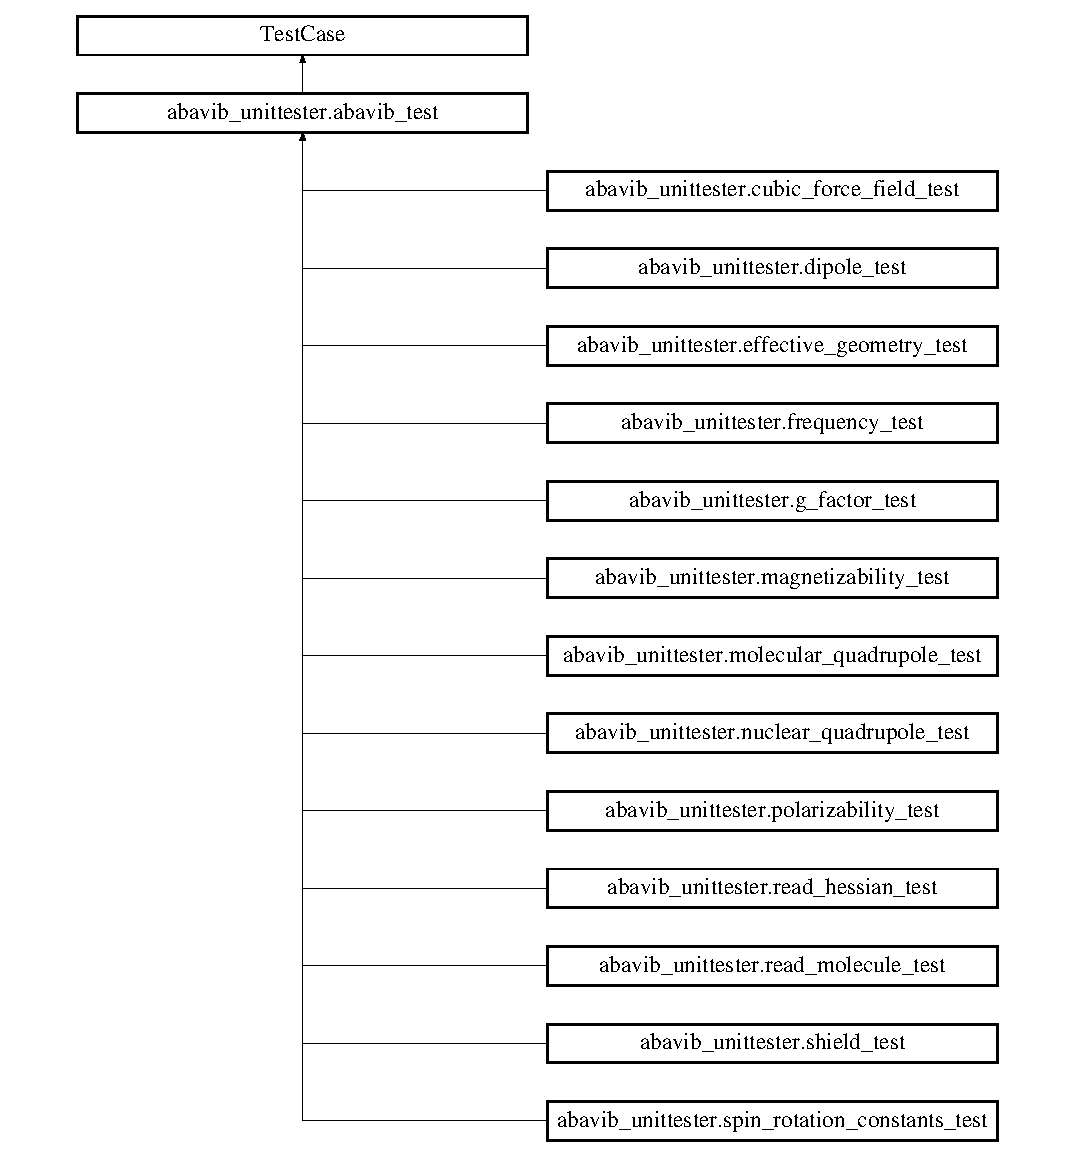
\includegraphics[height=12.000000cm]{classabavib__unittester_1_1abavib__test}
\end{center}
\end{figure}
\subsection*{Public Member Functions}
\begin{DoxyCompactItemize}
\item 
\hypertarget{classabavib__unittester_1_1abavib__test_a8aac0697aaa3a5cdf38ae39c9e4362c5}{def {\bfseries set\+Up}}\label{classabavib__unittester_1_1abavib__test_a8aac0697aaa3a5cdf38ae39c9e4362c5}

\end{DoxyCompactItemize}
\subsection*{Public Attributes}
\begin{DoxyCompactItemize}
\item 
\hypertarget{classabavib__unittester_1_1abavib__test_a6fa6ae385313c0c63bef6495beeec8c6}{{\bfseries molecule}}\label{classabavib__unittester_1_1abavib__test_a6fa6ae385313c0c63bef6495beeec8c6}

\item 
\hypertarget{classabavib__unittester_1_1abavib__test_a171cbc7ae0146803b6d9f0aca3d2ef5b}{{\bfseries input\+\_\+name}}\label{classabavib__unittester_1_1abavib__test_a171cbc7ae0146803b6d9f0aca3d2ef5b}

\item 
\hypertarget{classabavib__unittester_1_1abavib__test_a23dc9ba322b89932b6d11fe13ea2e9d0}{{\bfseries output\+\_\+file\+\_\+name}}\label{classabavib__unittester_1_1abavib__test_a23dc9ba322b89932b6d11fe13ea2e9d0}

\end{DoxyCompactItemize}
\subsection*{Static Public Attributes}
\begin{DoxyCompactItemize}
\item 
\hypertarget{classabavib__unittester_1_1abavib__test_aeb333ddfd05135d61cadeead74db8b3c}{string {\bfseries hessian\+\_\+name} = self.\+input\+\_\+name+'hessian'}\label{classabavib__unittester_1_1abavib__test_aeb333ddfd05135d61cadeead74db8b3c}

\item 
\hypertarget{classabavib__unittester_1_1abavib__test_aaa7889805632a7598f00c3ab8b8c4053}{tuple {\bfseries hessian\+\_\+t} = self.\+hessian.\+transpose()}\label{classabavib__unittester_1_1abavib__test_aaa7889805632a7598f00c3ab8b8c4053}

\item 
\hypertarget{classabavib__unittester_1_1abavib__test_ad036d56c040c6b2cd8ac548e0c26c72e}{tuple {\bfseries hessian\+\_\+temp} = np.\+add(self.\+hessian, hessian\+\_\+t)}\label{classabavib__unittester_1_1abavib__test_ad036d56c040c6b2cd8ac548e0c26c72e}

\item 
\hypertarget{classabavib__unittester_1_1abavib__test_aeefde93336cab151eb0bb2c1db4e5bd1}{tuple {\bfseries effective\+\_\+geometry\+\_\+norm} = av.\+effective\+\_\+geometry(self.\+cff\+\_\+norm\+\_\+reduced, self.\+freq, self.\+n\+\_\+atoms)}\label{classabavib__unittester_1_1abavib__test_aeefde93336cab151eb0bb2c1db4e5bd1}

\end{DoxyCompactItemize}


The documentation for this class was generated from the following file\+:\begin{DoxyCompactItemize}
\item 
abavib\+\_\+unittester.\+py\end{DoxyCompactItemize}

\hypertarget{classchiral__tester_1_1abavib__test}{\section{chiral\+\_\+tester.\+abavib\+\_\+test Class Reference}
\label{classchiral__tester_1_1abavib__test}\index{chiral\+\_\+tester.\+abavib\+\_\+test@{chiral\+\_\+tester.\+abavib\+\_\+test}}
}
Inheritance diagram for chiral\+\_\+tester.\+abavib\+\_\+test\+:\begin{figure}[H]
\begin{center}
\leavevmode
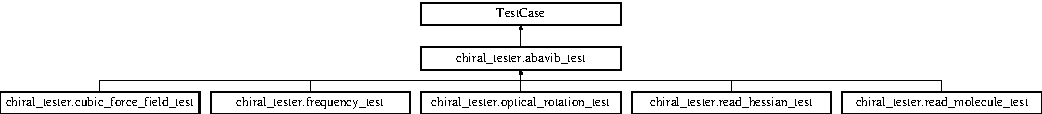
\includegraphics[height=1.534247cm]{classchiral__tester_1_1abavib__test}
\end{center}
\end{figure}
\subsection*{Public Member Functions}
\begin{DoxyCompactItemize}
\item 
\hypertarget{classchiral__tester_1_1abavib__test_a3abe45ea8e17ea9936776c832aac5cfb}{def {\bfseries set\+Up}}\label{classchiral__tester_1_1abavib__test_a3abe45ea8e17ea9936776c832aac5cfb}

\end{DoxyCompactItemize}
\subsection*{Static Public Attributes}
\begin{DoxyCompactItemize}
\item 
\hypertarget{classchiral__tester_1_1abavib__test_aa41e7bdb8a6b494a8e96274c2b97eba8}{string {\bfseries hessian\+\_\+name} = self.\+input\+\_\+name+'hessian'}\label{classchiral__tester_1_1abavib__test_aa41e7bdb8a6b494a8e96274c2b97eba8}

\item 
\hypertarget{classchiral__tester_1_1abavib__test_a3d2419940c78edc739e640754eaa0bb7}{tuple {\bfseries hessian\+\_\+t} = self.\+hessian.\+transpose()}\label{classchiral__tester_1_1abavib__test_a3d2419940c78edc739e640754eaa0bb7}

\item 
\hypertarget{classchiral__tester_1_1abavib__test_a9ca733f8f8484ac65ba00ef4403112c0}{tuple {\bfseries hessian\+\_\+temp} = np.\+add(self.\+hessian, hessian\+\_\+t)}\label{classchiral__tester_1_1abavib__test_a9ca733f8f8484ac65ba00ef4403112c0}

\end{DoxyCompactItemize}


The documentation for this class was generated from the following file\+:\begin{DoxyCompactItemize}
\item 
chiral\+\_\+tester.\+py\end{DoxyCompactItemize}

\hypertarget{classabavib__unittester_1_1cubic__force__field__test}{\section{abavib\+\_\+unittester.\+cubic\+\_\+force\+\_\+field\+\_\+test Class Reference}
\label{classabavib__unittester_1_1cubic__force__field__test}\index{abavib\+\_\+unittester.\+cubic\+\_\+force\+\_\+field\+\_\+test@{abavib\+\_\+unittester.\+cubic\+\_\+force\+\_\+field\+\_\+test}}
}
Inheritance diagram for abavib\+\_\+unittester.\+cubic\+\_\+force\+\_\+field\+\_\+test\+:\begin{figure}[H]
\begin{center}
\leavevmode
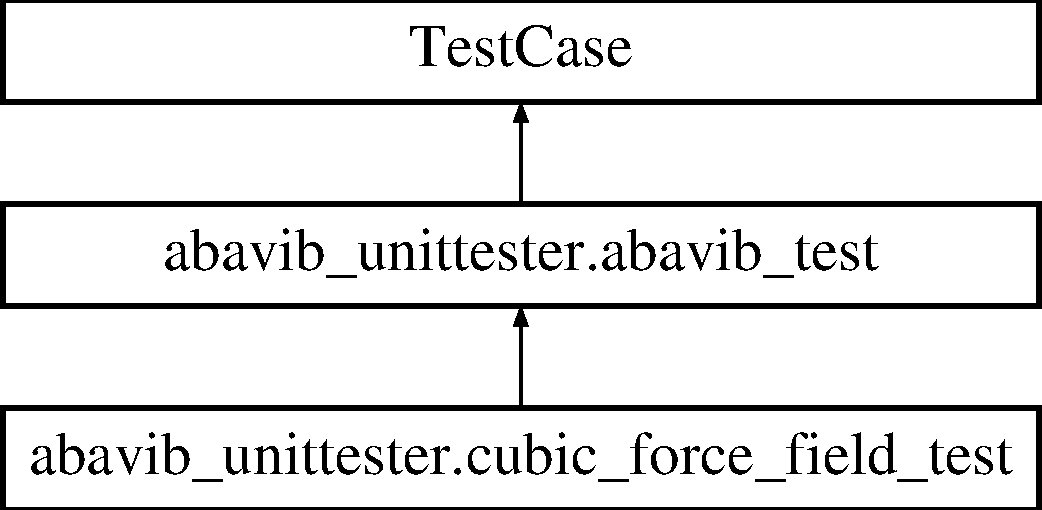
\includegraphics[height=3.000000cm]{classabavib__unittester_1_1cubic__force__field__test}
\end{center}
\end{figure}
\subsection*{Public Member Functions}
\begin{DoxyCompactItemize}
\item 
\hypertarget{classabavib__unittester_1_1cubic__force__field__test_a6d8a1ac55e92dab382535c172db37fe1}{def {\bfseries test\+\_\+cff}}\label{classabavib__unittester_1_1cubic__force__field__test_a6d8a1ac55e92dab382535c172db37fe1}

\end{DoxyCompactItemize}
\subsection*{Additional Inherited Members}


The documentation for this class was generated from the following file\+:\begin{DoxyCompactItemize}
\item 
abavib\+\_\+unittester.\+py\end{DoxyCompactItemize}

\hypertarget{classchiral__tester_1_1cubic__force__field__test}{\section{chiral\+\_\+tester.\+cubic\+\_\+force\+\_\+field\+\_\+test Class Reference}
\label{classchiral__tester_1_1cubic__force__field__test}\index{chiral\+\_\+tester.\+cubic\+\_\+force\+\_\+field\+\_\+test@{chiral\+\_\+tester.\+cubic\+\_\+force\+\_\+field\+\_\+test}}
}
Inheritance diagram for chiral\+\_\+tester.\+cubic\+\_\+force\+\_\+field\+\_\+test\+:\begin{figure}[H]
\begin{center}
\leavevmode
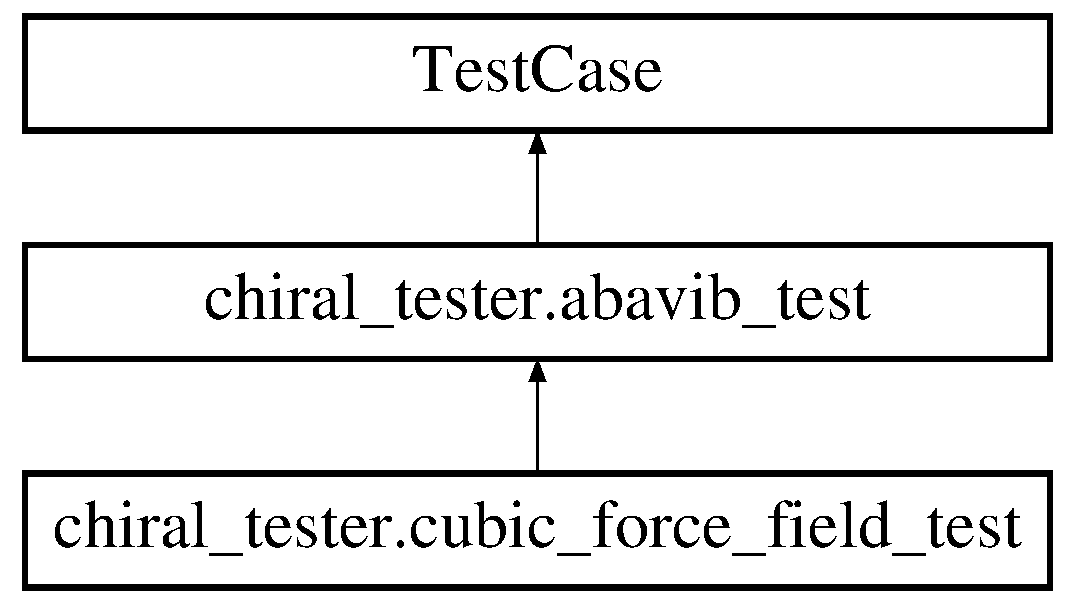
\includegraphics[height=3.000000cm]{classchiral__tester_1_1cubic__force__field__test}
\end{center}
\end{figure}
\subsection*{Public Member Functions}
\begin{DoxyCompactItemize}
\item 
\hypertarget{classchiral__tester_1_1cubic__force__field__test_ac7781a2d34591807e151814d40e82e66}{def {\bfseries test\+\_\+cff}}\label{classchiral__tester_1_1cubic__force__field__test_ac7781a2d34591807e151814d40e82e66}

\end{DoxyCompactItemize}
\subsection*{Additional Inherited Members}


The documentation for this class was generated from the following file\+:\begin{DoxyCompactItemize}
\item 
chiral\+\_\+tester.\+py\end{DoxyCompactItemize}

\hypertarget{classabavib__unittester_1_1dipole__test}{\section{abavib\+\_\+unittester.\+dipole\+\_\+test Class Reference}
\label{classabavib__unittester_1_1dipole__test}\index{abavib\+\_\+unittester.\+dipole\+\_\+test@{abavib\+\_\+unittester.\+dipole\+\_\+test}}
}
Inheritance diagram for abavib\+\_\+unittester.\+dipole\+\_\+test\+:\begin{figure}[H]
\begin{center}
\leavevmode
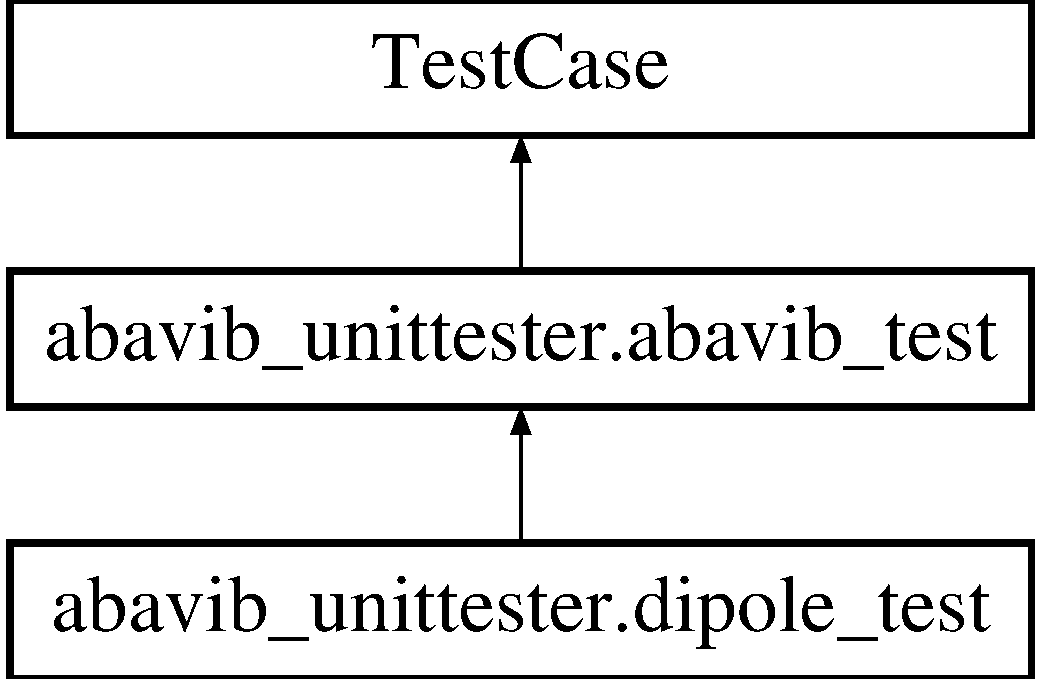
\includegraphics[height=3.000000cm]{classabavib__unittester_1_1dipole__test}
\end{center}
\end{figure}
\subsection*{Public Member Functions}
\begin{DoxyCompactItemize}
\item 
\hypertarget{classabavib__unittester_1_1dipole__test_a2c0f8a11c4637598a2da41f6d8239981}{def {\bfseries set\+Up}}\label{classabavib__unittester_1_1dipole__test_a2c0f8a11c4637598a2da41f6d8239981}

\item 
\hypertarget{classabavib__unittester_1_1dipole__test_a8be7710eb8af478ce6484e7030cf3309}{def {\bfseries test\+\_\+dipole\+\_\+corrections}}\label{classabavib__unittester_1_1dipole__test_a8be7710eb8af478ce6484e7030cf3309}

\item 
\hypertarget{classabavib__unittester_1_1dipole__test_a49bd584afe5ab540c023fd941f56eef2}{def {\bfseries test\+\_\+dipole\+\_\+moment}}\label{classabavib__unittester_1_1dipole__test_a49bd584afe5ab540c023fd941f56eef2}

\end{DoxyCompactItemize}
\subsection*{Public Attributes}
\begin{DoxyCompactItemize}
\item 
\hypertarget{classabavib__unittester_1_1dipole__test_a2704463450130b37abb2a97a078feae0}{{\bfseries corrected\+\_\+values}}\label{classabavib__unittester_1_1dipole__test_a2704463450130b37abb2a97a078feae0}

\item 
\hypertarget{classabavib__unittester_1_1dipole__test_a331c16d1033ae7c8c7f8cb509571c6d9}{{\bfseries dipole\+\_\+moment\+\_\+corrected}}\label{classabavib__unittester_1_1dipole__test_a331c16d1033ae7c8c7f8cb509571c6d9}

\item 
\hypertarget{classabavib__unittester_1_1dipole__test_ac673e906d28924b83550f5a3641bb1f3}{{\bfseries molecule}}\label{classabavib__unittester_1_1dipole__test_ac673e906d28924b83550f5a3641bb1f3}

\end{DoxyCompactItemize}
\subsection*{Additional Inherited Members}


The documentation for this class was generated from the following file\+:\begin{DoxyCompactItemize}
\item 
abavib\+\_\+unittester.\+py\end{DoxyCompactItemize}

\hypertarget{classabavib__unittester_1_1effective__geometry__test}{\section{abavib\+\_\+unittester.\+effective\+\_\+geometry\+\_\+test Class Reference}
\label{classabavib__unittester_1_1effective__geometry__test}\index{abavib\+\_\+unittester.\+effective\+\_\+geometry\+\_\+test@{abavib\+\_\+unittester.\+effective\+\_\+geometry\+\_\+test}}
}
Inheritance diagram for abavib\+\_\+unittester.\+effective\+\_\+geometry\+\_\+test\+:\begin{figure}[H]
\begin{center}
\leavevmode
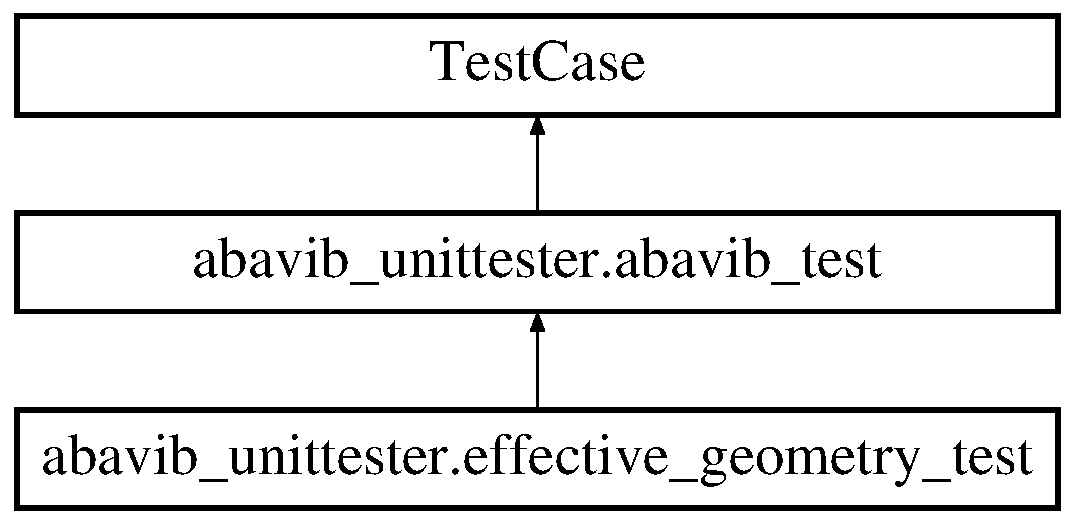
\includegraphics[height=3.000000cm]{classabavib__unittester_1_1effective__geometry__test}
\end{center}
\end{figure}
\subsection*{Public Member Functions}
\begin{DoxyCompactItemize}
\item 
\hypertarget{classabavib__unittester_1_1effective__geometry__test_ae467da78c37ec40a981481975b598472}{def {\bfseries test\+\_\+effective\+\_\+geometry}}\label{classabavib__unittester_1_1effective__geometry__test_ae467da78c37ec40a981481975b598472}

\end{DoxyCompactItemize}
\subsection*{Public Attributes}
\begin{DoxyCompactItemize}
\item 
\hypertarget{classabavib__unittester_1_1effective__geometry__test_a11e284ee455dae8ed16cc16b3343ceae}{{\bfseries molecule}}\label{classabavib__unittester_1_1effective__geometry__test_a11e284ee455dae8ed16cc16b3343ceae}

\end{DoxyCompactItemize}
\subsection*{Additional Inherited Members}


The documentation for this class was generated from the following file\+:\begin{DoxyCompactItemize}
\item 
abavib\+\_\+unittester.\+py\end{DoxyCompactItemize}

\hypertarget{classelement_1_1Element}{\section{element.\+Element Class Reference}
\label{classelement_1_1Element}\index{element.\+Element@{element.\+Element}}
}
Inheritance diagram for element.\+Element\+:\begin{figure}[H]
\begin{center}
\leavevmode
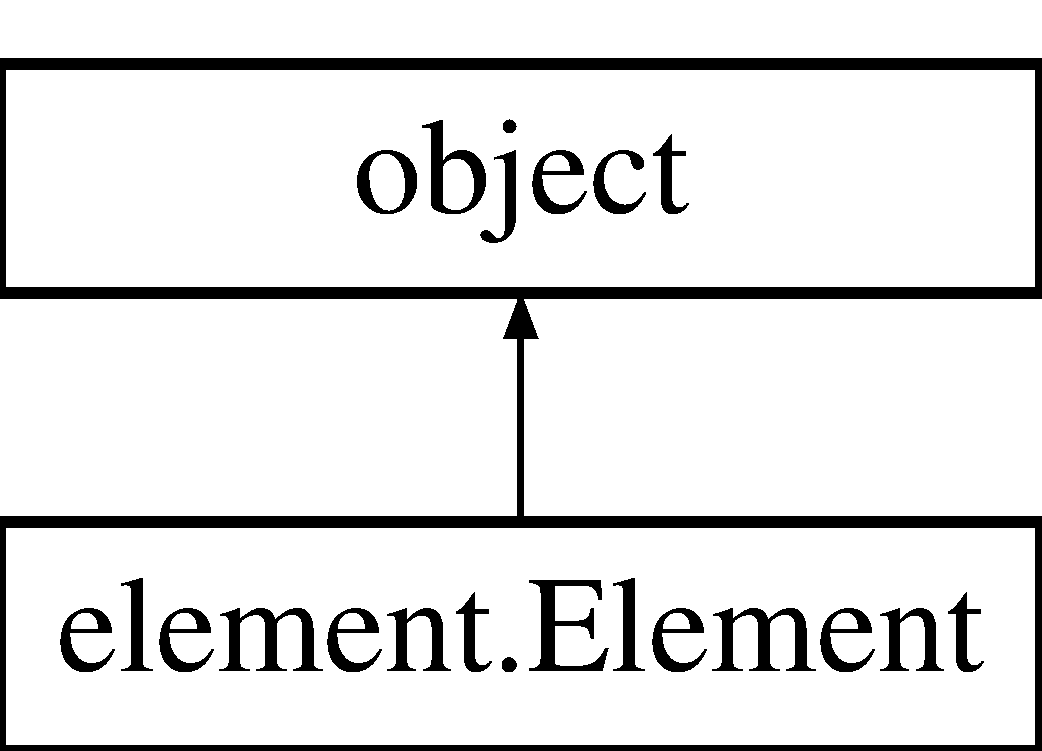
\includegraphics[height=2.000000cm]{classelement_1_1Element}
\end{center}
\end{figure}
\subsection*{Public Member Functions}
\begin{DoxyCompactItemize}
\item 
\hypertarget{classelement_1_1Element_afdc7b7986e3d6aad311573f3c2534b85}{def {\bfseries \+\_\+\+\_\+init\+\_\+\+\_\+}}\label{classelement_1_1Element_afdc7b7986e3d6aad311573f3c2534b85}

\item 
\hypertarget{classelement_1_1Element_a742f94002c18f60d4a3c384b51925c69}{def {\bfseries \+\_\+\+\_\+str\+\_\+\+\_\+}}\label{classelement_1_1Element_a742f94002c18f60d4a3c384b51925c69}

\item 
\hypertarget{classelement_1_1Element_ae1907c0f9d227680d5adbbe043319439}{def {\bfseries \+\_\+\+\_\+repr\+\_\+\+\_\+}}\label{classelement_1_1Element_ae1907c0f9d227680d5adbbe043319439}

\item 
def \hyperlink{classelement_1_1Element_a03f0d947587085800e751ca03b6be838}{nominalmass}
\item 
def \hyperlink{classelement_1_1Element_a724eecca89aa1b702bc28e4f677c153b}{neutrons}
\item 
def \hyperlink{classelement_1_1Element_ad8a714b6fff3ff4fecfaaa18a0a154b0}{exactmass}
\item 
def \hyperlink{classelement_1_1Element_a79948ad87c3aca7399fc020751237816}{eleconfig\+\_\+dict}
\item 
def \hyperlink{classelement_1_1Element_aaf89f4509db83e7b508684d406e6c424}{eleshells}
\item 
def \hyperlink{classelement_1_1Element_afa89449c3f12453d39aba4c0b4c3231b}{description}
\item 
def \hyperlink{classelement_1_1Element_a5b38ca7d1691ffca9dc6f1a52c479dec}{validate}
\end{DoxyCompactItemize}
\subsection*{Public Attributes}
\begin{DoxyCompactItemize}
\item 
\hypertarget{classelement_1_1Element_aaeca0589842140bcf2d857b869a45eb6}{{\bfseries number}}\label{classelement_1_1Element_aaeca0589842140bcf2d857b869a45eb6}

\item 
\hypertarget{classelement_1_1Element_ac338f4eb7a42fcdb7568b5d65cbb2536}{{\bfseries symbol}}\label{classelement_1_1Element_ac338f4eb7a42fcdb7568b5d65cbb2536}

\item 
\hypertarget{classelement_1_1Element_ae50faae6487ac44a57bf588d19c03153}{{\bfseries name}}\label{classelement_1_1Element_ae50faae6487ac44a57bf588d19c03153}

\item 
\hypertarget{classelement_1_1Element_acaf8dec84fb6f0e21a9e18e0ac0f9603}{{\bfseries electrons}}\label{classelement_1_1Element_acaf8dec84fb6f0e21a9e18e0ac0f9603}

\item 
\hypertarget{classelement_1_1Element_aeb808cc01a4c2f63a8291abe5674d904}{{\bfseries protons}}\label{classelement_1_1Element_aeb808cc01a4c2f63a8291abe5674d904}

\end{DoxyCompactItemize}


\subsection{Detailed Description}
\begin{DoxyVerb}Chemical element.

Attributes
----------
number : int
    Atomic number
symbol : str of length 1 or 2
    Chemical symbol
name : str
    Name in english
group : int
    Group in periodic table
period : int
    Period in periodic table
block : int
    Block in periodic table
series : int
    Index to chemical series
protons : int
    Number of protons
neutrons : int
    Number of neutrons in the most abundant naturally occurring stable
    isotope
nominalmass : int
    Mass number of the most abundant naturally occurring stable isotope
electrons : int
    Number of electrons
mass : float
    Relative atomic mass. Ratio of the average mass of atoms
    of the element to 1/12 of the mass of an atom of 12C
exactmass : float
    Relative atomic mass calculated from the isotopic composition
eleneg : float
    Electronegativity (Pauling scale)
covrad : float
    Covalent radius in Angstrom
atmrad :
    Atomic radius in Angstrom
vdwrad : float
    Van der Waals radius in Angstrom
tboil : float
    Boiling temperature in K
tmelt : float
    Melting temperature in K
density : float
    Density at 295K in g/cm3 respectively g/L
oxistates : str
    Oxidation states
eleaffin : float
    Electron affinity in eV
eleconfig : str
    Ground state electron configuration
eleconfig_dict : dict
    Ground state electron configuration (shell, subshell): electrons
eleshells : int
    Number of electrons per shell
ionenergy : tuple
    Ionization energies in eV
isotopes : dict
    Isotopic composition.
    keys: isotope mass number
    values: Isotope(relative atomic mass, abundance)\end{DoxyVerb}
 

\subsection{Member Function Documentation}
\hypertarget{classelement_1_1Element_afa89449c3f12453d39aba4c0b4c3231b}{\index{element\+::\+Element@{element\+::\+Element}!description@{description}}
\index{description@{description}!element\+::\+Element@{element\+::\+Element}}
\subsubsection[{description}]{\setlength{\rightskip}{0pt plus 5cm}def element.\+Element.\+description (
\begin{DoxyParamCaption}
\item[{}]{self}
\end{DoxyParamCaption}
)}}\label{classelement_1_1Element_afa89449c3f12453d39aba4c0b4c3231b}
\begin{DoxyVerb}Return text description of element.\end{DoxyVerb}
 \hypertarget{classelement_1_1Element_a79948ad87c3aca7399fc020751237816}{\index{element\+::\+Element@{element\+::\+Element}!eleconfig\+\_\+dict@{eleconfig\+\_\+dict}}
\index{eleconfig\+\_\+dict@{eleconfig\+\_\+dict}!element\+::\+Element@{element\+::\+Element}}
\subsubsection[{eleconfig\+\_\+dict}]{\setlength{\rightskip}{0pt plus 5cm}def element.\+Element.\+eleconfig\+\_\+dict (
\begin{DoxyParamCaption}
\item[{}]{self}
\end{DoxyParamCaption}
)}}\label{classelement_1_1Element_a79948ad87c3aca7399fc020751237816}
\begin{DoxyVerb}Return electron configuration as dict.\end{DoxyVerb}
 \hypertarget{classelement_1_1Element_aaf89f4509db83e7b508684d406e6c424}{\index{element\+::\+Element@{element\+::\+Element}!eleshells@{eleshells}}
\index{eleshells@{eleshells}!element\+::\+Element@{element\+::\+Element}}
\subsubsection[{eleshells}]{\setlength{\rightskip}{0pt plus 5cm}def element.\+Element.\+eleshells (
\begin{DoxyParamCaption}
\item[{}]{self}
\end{DoxyParamCaption}
)}}\label{classelement_1_1Element_aaf89f4509db83e7b508684d406e6c424}
\begin{DoxyVerb}Return number of electrons in shell as tuple.\end{DoxyVerb}
 \hypertarget{classelement_1_1Element_ad8a714b6fff3ff4fecfaaa18a0a154b0}{\index{element\+::\+Element@{element\+::\+Element}!exactmass@{exactmass}}
\index{exactmass@{exactmass}!element\+::\+Element@{element\+::\+Element}}
\subsubsection[{exactmass}]{\setlength{\rightskip}{0pt plus 5cm}def element.\+Element.\+exactmass (
\begin{DoxyParamCaption}
\item[{}]{self}
\end{DoxyParamCaption}
)}}\label{classelement_1_1Element_ad8a714b6fff3ff4fecfaaa18a0a154b0}
\begin{DoxyVerb}Return relative atomic mass calculated from isotopic composition.\end{DoxyVerb}
 \hypertarget{classelement_1_1Element_a724eecca89aa1b702bc28e4f677c153b}{\index{element\+::\+Element@{element\+::\+Element}!neutrons@{neutrons}}
\index{neutrons@{neutrons}!element\+::\+Element@{element\+::\+Element}}
\subsubsection[{neutrons}]{\setlength{\rightskip}{0pt plus 5cm}def element.\+Element.\+neutrons (
\begin{DoxyParamCaption}
\item[{}]{self}
\end{DoxyParamCaption}
)}}\label{classelement_1_1Element_a724eecca89aa1b702bc28e4f677c153b}
\begin{DoxyVerb}Return number neutrons in most abundant natural stable isotope.\end{DoxyVerb}
 \hypertarget{classelement_1_1Element_a03f0d947587085800e751ca03b6be838}{\index{element\+::\+Element@{element\+::\+Element}!nominalmass@{nominalmass}}
\index{nominalmass@{nominalmass}!element\+::\+Element@{element\+::\+Element}}
\subsubsection[{nominalmass}]{\setlength{\rightskip}{0pt plus 5cm}def element.\+Element.\+nominalmass (
\begin{DoxyParamCaption}
\item[{}]{self}
\end{DoxyParamCaption}
)}}\label{classelement_1_1Element_a03f0d947587085800e751ca03b6be838}
\begin{DoxyVerb}Return mass number of most abundant natural stable isotope.\end{DoxyVerb}
 \hypertarget{classelement_1_1Element_a5b38ca7d1691ffca9dc6f1a52c479dec}{\index{element\+::\+Element@{element\+::\+Element}!validate@{validate}}
\index{validate@{validate}!element\+::\+Element@{element\+::\+Element}}
\subsubsection[{validate}]{\setlength{\rightskip}{0pt plus 5cm}def element.\+Element.\+validate (
\begin{DoxyParamCaption}
\item[{}]{self}
\end{DoxyParamCaption}
)}}\label{classelement_1_1Element_a5b38ca7d1691ffca9dc6f1a52c479dec}
\begin{DoxyVerb}Check consistency of data. Raise Error on failure.\end{DoxyVerb}
 

The documentation for this class was generated from the following file\+:\begin{DoxyCompactItemize}
\item 
element.\+py\end{DoxyCompactItemize}

\hypertarget{classelement_1_1ElementsDict}{\section{element.\+Elements\+Dict Class Reference}
\label{classelement_1_1ElementsDict}\index{element.\+Elements\+Dict@{element.\+Elements\+Dict}}
}
Inheritance diagram for element.\+Elements\+Dict\+:\begin{figure}[H]
\begin{center}
\leavevmode
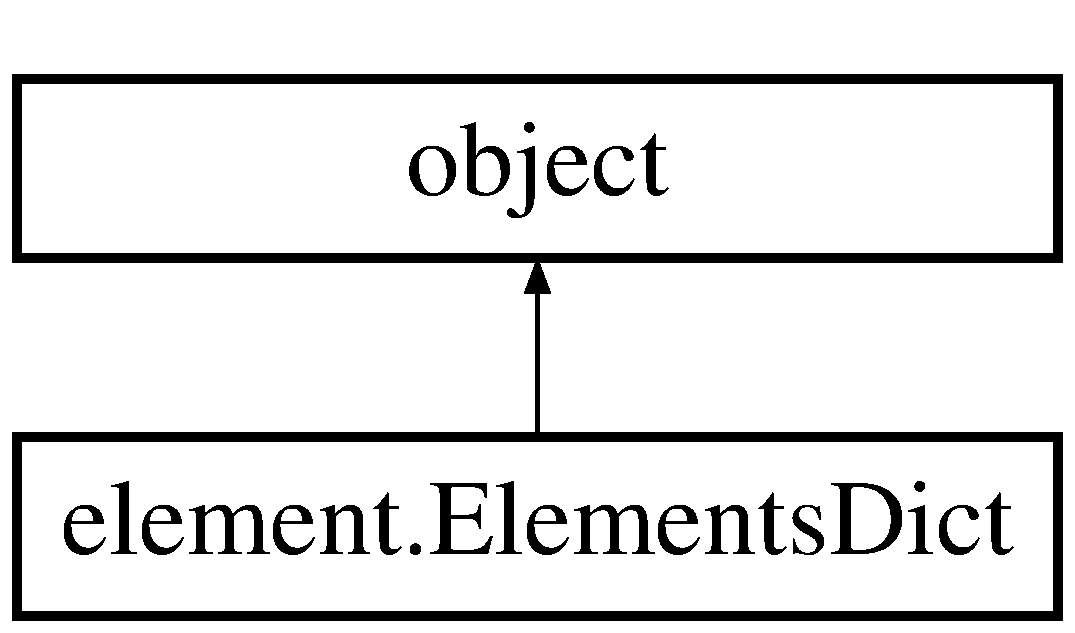
\includegraphics[height=2.000000cm]{classelement_1_1ElementsDict}
\end{center}
\end{figure}
\subsection*{Public Member Functions}
\begin{DoxyCompactItemize}
\item 
\hypertarget{classelement_1_1ElementsDict_a1651fb045c87b116643c9ed3534a86ce}{def {\bfseries \+\_\+\+\_\+init\+\_\+\+\_\+}}\label{classelement_1_1ElementsDict_a1651fb045c87b116643c9ed3534a86ce}

\item 
\hypertarget{classelement_1_1ElementsDict_a74aee0774c62e6c87584e0d89d3b6704}{def {\bfseries \+\_\+\+\_\+str\+\_\+\+\_\+}}\label{classelement_1_1ElementsDict_a74aee0774c62e6c87584e0d89d3b6704}

\item 
\hypertarget{classelement_1_1ElementsDict_aa69d6a81b2a5051a6973126f9a2820b2}{def {\bfseries \+\_\+\+\_\+contains\+\_\+\+\_\+}}\label{classelement_1_1ElementsDict_aa69d6a81b2a5051a6973126f9a2820b2}

\item 
\hypertarget{classelement_1_1ElementsDict_a988599b55550e0707d9e2a3f2663ad67}{def {\bfseries \+\_\+\+\_\+iter\+\_\+\+\_\+}}\label{classelement_1_1ElementsDict_a988599b55550e0707d9e2a3f2663ad67}

\item 
\hypertarget{classelement_1_1ElementsDict_a9711622a1159982e5f1651381f764a7c}{def {\bfseries \+\_\+\+\_\+len\+\_\+\+\_\+}}\label{classelement_1_1ElementsDict_a9711622a1159982e5f1651381f764a7c}

\item 
\hypertarget{classelement_1_1ElementsDict_afa50a6c81f087a365b85fac399c5e399}{def {\bfseries \+\_\+\+\_\+getitem\+\_\+\+\_\+}}\label{classelement_1_1ElementsDict_afa50a6c81f087a365b85fac399c5e399}

\end{DoxyCompactItemize}


\subsection{Detailed Description}
\begin{DoxyVerb}Ordered dict of Elements with lookup by number, symbol, and name.\end{DoxyVerb}
 

The documentation for this class was generated from the following file\+:\begin{DoxyCompactItemize}
\item 
element.\+py\end{DoxyCompactItemize}

\hypertarget{classchiral__tester_1_1frequency__test}{\section{chiral\+\_\+tester.\+frequency\+\_\+test Class Reference}
\label{classchiral__tester_1_1frequency__test}\index{chiral\+\_\+tester.\+frequency\+\_\+test@{chiral\+\_\+tester.\+frequency\+\_\+test}}
}
Inheritance diagram for chiral\+\_\+tester.\+frequency\+\_\+test\+:\begin{figure}[H]
\begin{center}
\leavevmode
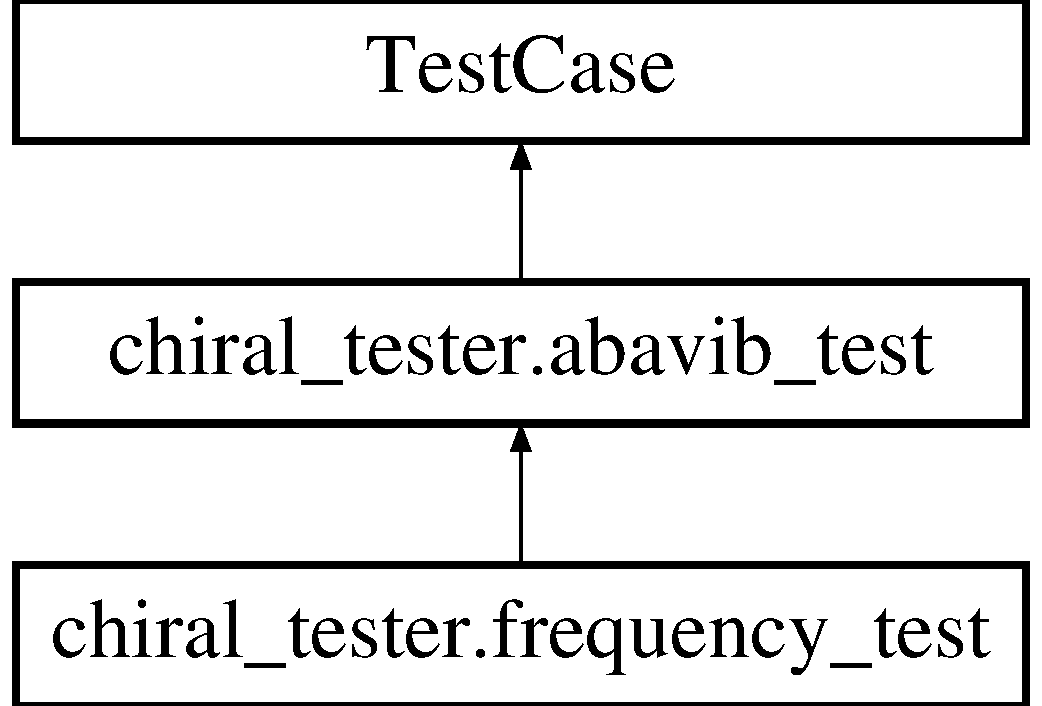
\includegraphics[height=3.000000cm]{classchiral__tester_1_1frequency__test}
\end{center}
\end{figure}
\subsection*{Public Member Functions}
\begin{DoxyCompactItemize}
\item 
\hypertarget{classchiral__tester_1_1frequency__test_a9be6690b1abb3f183b82427b62c90fdd}{def {\bfseries test\+\_\+frequencies}}\label{classchiral__tester_1_1frequency__test_a9be6690b1abb3f183b82427b62c90fdd}

\item 
\hypertarget{classchiral__tester_1_1frequency__test_a6165a8c07f6c474b0a964bfc65209300}{def {\bfseries test\+\_\+eigvec}}\label{classchiral__tester_1_1frequency__test_a6165a8c07f6c474b0a964bfc65209300}

\end{DoxyCompactItemize}
\subsection*{Public Attributes}
\begin{DoxyCompactItemize}
\item 
\hypertarget{classchiral__tester_1_1frequency__test_a9da6c7e36728ca8a521776da8a823cd8}{{\bfseries molecule}}\label{classchiral__tester_1_1frequency__test_a9da6c7e36728ca8a521776da8a823cd8}

\item 
\hypertarget{classchiral__tester_1_1frequency__test_aacc963809144e88a62e50ef9273704df}{{\bfseries eigvec}}\label{classchiral__tester_1_1frequency__test_aacc963809144e88a62e50ef9273704df}

\end{DoxyCompactItemize}
\subsection*{Additional Inherited Members}


The documentation for this class was generated from the following file\+:\begin{DoxyCompactItemize}
\item 
chiral\+\_\+tester.\+py\end{DoxyCompactItemize}

\hypertarget{classabavib__unittester_1_1frequency__test}{\section{abavib\+\_\+unittester.\+frequency\+\_\+test Class Reference}
\label{classabavib__unittester_1_1frequency__test}\index{abavib\+\_\+unittester.\+frequency\+\_\+test@{abavib\+\_\+unittester.\+frequency\+\_\+test}}
}
Inheritance diagram for abavib\+\_\+unittester.\+frequency\+\_\+test\+:\begin{figure}[H]
\begin{center}
\leavevmode
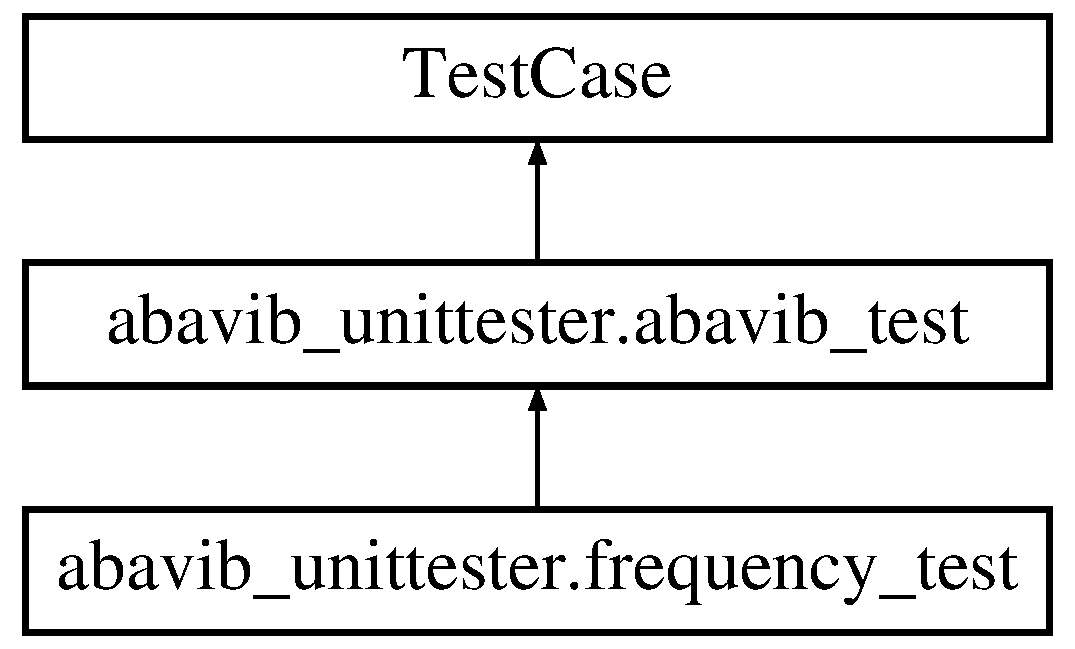
\includegraphics[height=3.000000cm]{classabavib__unittester_1_1frequency__test}
\end{center}
\end{figure}
\subsection*{Public Member Functions}
\begin{DoxyCompactItemize}
\item 
\hypertarget{classabavib__unittester_1_1frequency__test_a8fbdf092f714ef93e37372c969a69b11}{def {\bfseries test\+\_\+frequencies}}\label{classabavib__unittester_1_1frequency__test_a8fbdf092f714ef93e37372c969a69b11}

\item 
\hypertarget{classabavib__unittester_1_1frequency__test_aa92a00e3b45c51000469f5a1484ef31d}{def {\bfseries test\+\_\+eigvec}}\label{classabavib__unittester_1_1frequency__test_aa92a00e3b45c51000469f5a1484ef31d}

\end{DoxyCompactItemize}
\subsection*{Public Attributes}
\begin{DoxyCompactItemize}
\item 
\hypertarget{classabavib__unittester_1_1frequency__test_a4b964bb6cb824031746a950976d11502}{{\bfseries molecule}}\label{classabavib__unittester_1_1frequency__test_a4b964bb6cb824031746a950976d11502}

\item 
\hypertarget{classabavib__unittester_1_1frequency__test_ad908bea16d6dab17748c275cbe6a013b}{{\bfseries eigvec}}\label{classabavib__unittester_1_1frequency__test_ad908bea16d6dab17748c275cbe6a013b}

\end{DoxyCompactItemize}
\subsection*{Additional Inherited Members}


The documentation for this class was generated from the following file\+:\begin{DoxyCompactItemize}
\item 
abavib\+\_\+unittester.\+py\end{DoxyCompactItemize}

\hypertarget{classabavib__unittester_1_1g__factor__test}{\section{abavib\+\_\+unittester.\+g\+\_\+factor\+\_\+test Class Reference}
\label{classabavib__unittester_1_1g__factor__test}\index{abavib\+\_\+unittester.\+g\+\_\+factor\+\_\+test@{abavib\+\_\+unittester.\+g\+\_\+factor\+\_\+test}}
}
Inheritance diagram for abavib\+\_\+unittester.\+g\+\_\+factor\+\_\+test\+:\begin{figure}[H]
\begin{center}
\leavevmode
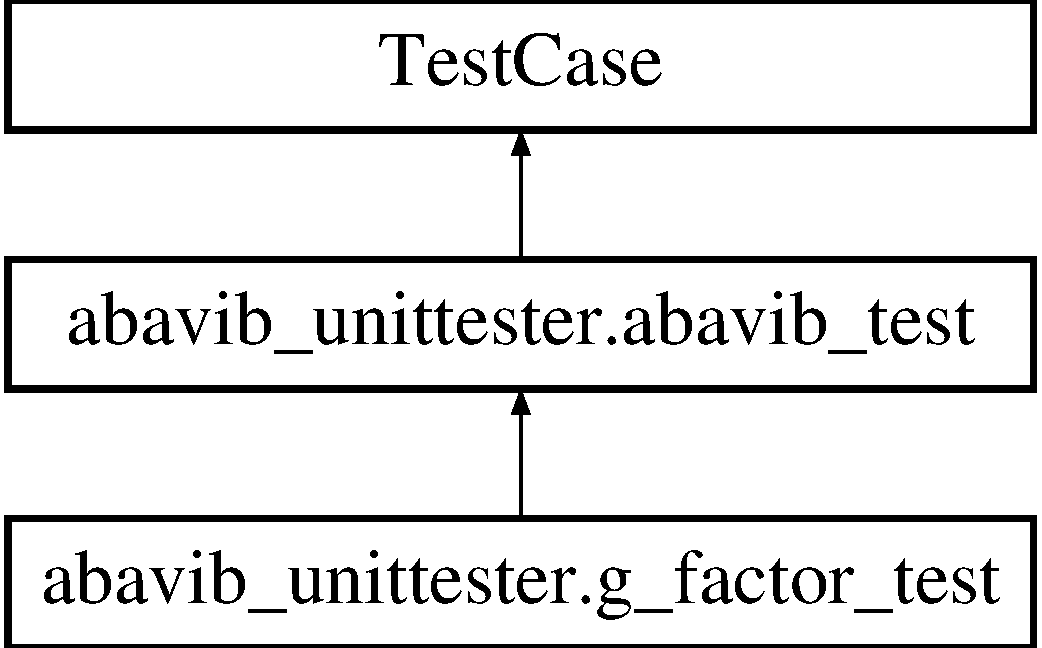
\includegraphics[height=3.000000cm]{classabavib__unittester_1_1g__factor__test}
\end{center}
\end{figure}
\subsection*{Public Member Functions}
\begin{DoxyCompactItemize}
\item 
\hypertarget{classabavib__unittester_1_1g__factor__test_a44307c525420d269bafcd5c08135dcd2}{def {\bfseries set\+Up}}\label{classabavib__unittester_1_1g__factor__test_a44307c525420d269bafcd5c08135dcd2}

\item 
\hypertarget{classabavib__unittester_1_1g__factor__test_ae8ce115d02e8273436b0de4e911bd9d5}{def {\bfseries test\+\_\+g\+\_\+factor\+\_\+corrections}}\label{classabavib__unittester_1_1g__factor__test_ae8ce115d02e8273436b0de4e911bd9d5}

\item 
\hypertarget{classabavib__unittester_1_1g__factor__test_a74eca9dd1aefb68f8f640ebf7333e55b}{def {\bfseries test\+\_\+g\+\_\+factor\+\_\+values}}\label{classabavib__unittester_1_1g__factor__test_a74eca9dd1aefb68f8f640ebf7333e55b}

\end{DoxyCompactItemize}
\subsection*{Public Attributes}
\begin{DoxyCompactItemize}
\item 
\hypertarget{classabavib__unittester_1_1g__factor__test_a890e6cdd38d247f49adb596a69af14e6}{{\bfseries corrected\+\_\+values}}\label{classabavib__unittester_1_1g__factor__test_a890e6cdd38d247f49adb596a69af14e6}

\item 
\hypertarget{classabavib__unittester_1_1g__factor__test_af85acd64376d0d28fe878aaa8f0d2cfa}{{\bfseries g\+\_\+factor}}\label{classabavib__unittester_1_1g__factor__test_af85acd64376d0d28fe878aaa8f0d2cfa}

\item 
\hypertarget{classabavib__unittester_1_1g__factor__test_a9d68d9437ecb32350670facd5779437c}{{\bfseries molecule}}\label{classabavib__unittester_1_1g__factor__test_a9d68d9437ecb32350670facd5779437c}

\end{DoxyCompactItemize}
\subsection*{Additional Inherited Members}


The documentation for this class was generated from the following file\+:\begin{DoxyCompactItemize}
\item 
abavib\+\_\+unittester.\+py\end{DoxyCompactItemize}

\hypertarget{classelement_1_1Isotope}{\section{element.\+Isotope Class Reference}
\label{classelement_1_1Isotope}\index{element.\+Isotope@{element.\+Isotope}}
}
Inheritance diagram for element.\+Isotope\+:\begin{figure}[H]
\begin{center}
\leavevmode
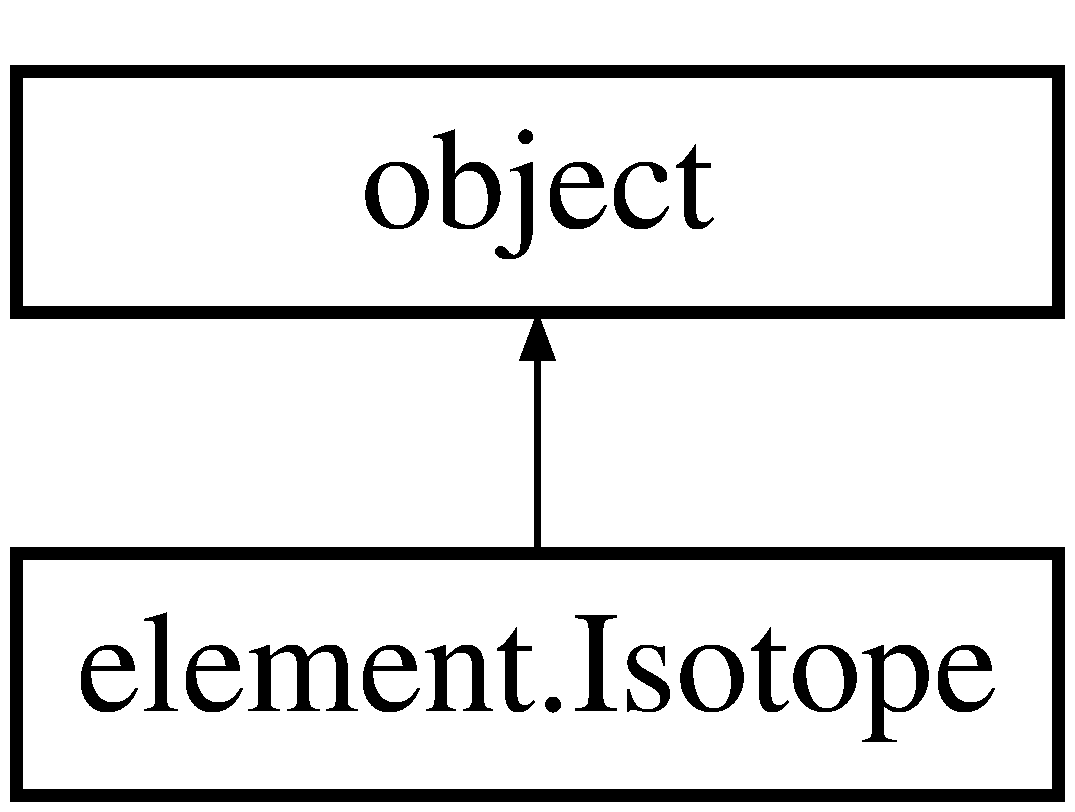
\includegraphics[height=2.000000cm]{classelement_1_1Isotope}
\end{center}
\end{figure}
\subsection*{Public Member Functions}
\begin{DoxyCompactItemize}
\item 
\hypertarget{classelement_1_1Isotope_abf01a2a4f218cba0e54533d7240778f3}{def {\bfseries \+\_\+\+\_\+init\+\_\+\+\_\+}}\label{classelement_1_1Isotope_abf01a2a4f218cba0e54533d7240778f3}

\item 
\hypertarget{classelement_1_1Isotope_a361f52e572b72eac4262e9de6609cfb2}{def {\bfseries \+\_\+\+\_\+str\+\_\+\+\_\+}}\label{classelement_1_1Isotope_a361f52e572b72eac4262e9de6609cfb2}

\item 
\hypertarget{classelement_1_1Isotope_a7528e92c63317a8a8c5674c2db36966b}{def {\bfseries \+\_\+\+\_\+repr\+\_\+\+\_\+}}\label{classelement_1_1Isotope_a7528e92c63317a8a8c5674c2db36966b}

\end{DoxyCompactItemize}
\subsection*{Public Attributes}
\begin{DoxyCompactItemize}
\item 
\hypertarget{classelement_1_1Isotope_a2e31ac3e98b35a5397b6b8436616a508}{{\bfseries mass}}\label{classelement_1_1Isotope_a2e31ac3e98b35a5397b6b8436616a508}

\item 
\hypertarget{classelement_1_1Isotope_ab8adfe46b387505f9dd6531aba9d7bb1}{{\bfseries abundance}}\label{classelement_1_1Isotope_ab8adfe46b387505f9dd6531aba9d7bb1}

\item 
\hypertarget{classelement_1_1Isotope_ae91f09ed3099994069bae0718618e027}{{\bfseries massnumber}}\label{classelement_1_1Isotope_ae91f09ed3099994069bae0718618e027}

\end{DoxyCompactItemize}


\subsection{Detailed Description}
\begin{DoxyVerb}Isotope massnumber, relative atomic mass, and abundance.\end{DoxyVerb}
 

The documentation for this class was generated from the following file\+:\begin{DoxyCompactItemize}
\item 
element.\+py\end{DoxyCompactItemize}

\hypertarget{classelement_1_1lazyattr}{\section{element.\+lazyattr Class Reference}
\label{classelement_1_1lazyattr}\index{element.\+lazyattr@{element.\+lazyattr}}
}
Inheritance diagram for element.\+lazyattr\+:\begin{figure}[H]
\begin{center}
\leavevmode
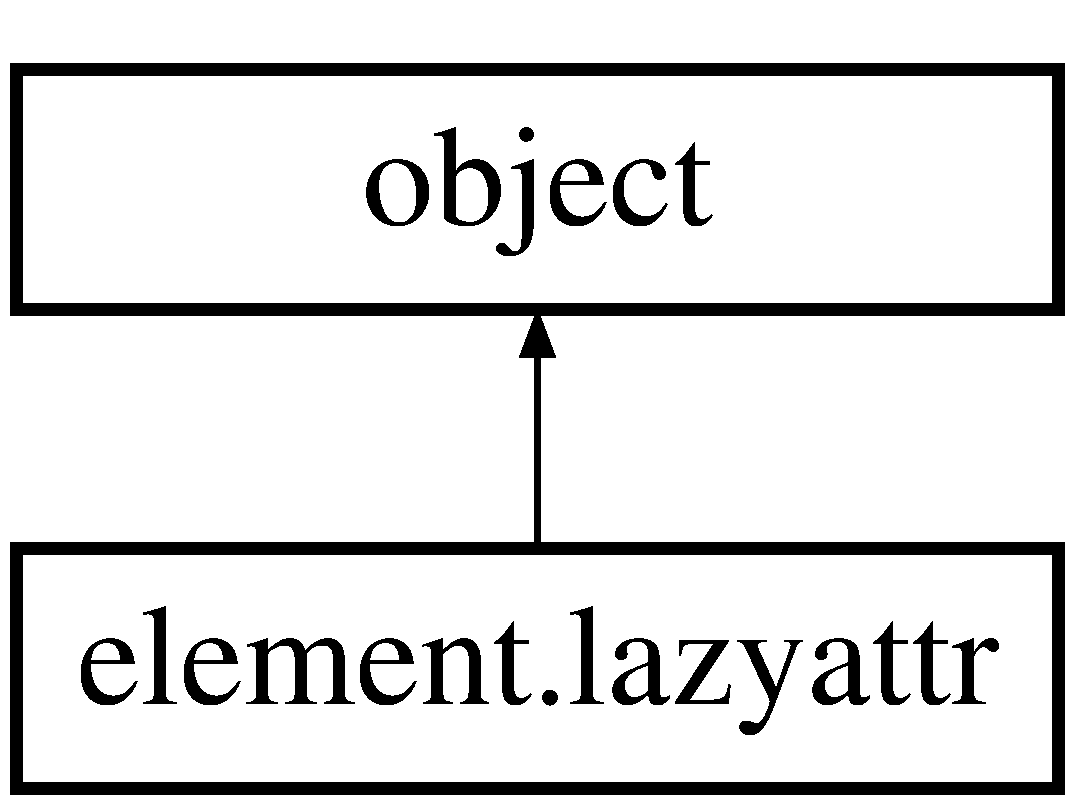
\includegraphics[height=2.000000cm]{classelement_1_1lazyattr}
\end{center}
\end{figure}
\subsection*{Public Member Functions}
\begin{DoxyCompactItemize}
\item 
\hypertarget{classelement_1_1lazyattr_abe019bda74dcf6f487eb1cc2da614586}{def {\bfseries \+\_\+\+\_\+init\+\_\+\+\_\+}}\label{classelement_1_1lazyattr_abe019bda74dcf6f487eb1cc2da614586}

\item 
\hypertarget{classelement_1_1lazyattr_a550ef7410b7407ce6b410787efd2e2de}{def {\bfseries \+\_\+\+\_\+get\+\_\+\+\_\+}}\label{classelement_1_1lazyattr_a550ef7410b7407ce6b410787efd2e2de}

\end{DoxyCompactItemize}
\subsection*{Public Attributes}
\begin{DoxyCompactItemize}
\item 
\hypertarget{classelement_1_1lazyattr_abc53ebd33f56c2eb6c2de6f2400aeda2}{{\bfseries func}}\label{classelement_1_1lazyattr_abc53ebd33f56c2eb6c2de6f2400aeda2}

\end{DoxyCompactItemize}


\subsection{Detailed Description}
\begin{DoxyVerb}Lazy object attribute whose value is computed on first access.\end{DoxyVerb}
 

The documentation for this class was generated from the following file\+:\begin{DoxyCompactItemize}
\item 
element.\+py\end{DoxyCompactItemize}

\hypertarget{classabavib__unittester_1_1magnetizability__test}{\section{abavib\+\_\+unittester.\+magnetizability\+\_\+test Class Reference}
\label{classabavib__unittester_1_1magnetizability__test}\index{abavib\+\_\+unittester.\+magnetizability\+\_\+test@{abavib\+\_\+unittester.\+magnetizability\+\_\+test}}
}
Inheritance diagram for abavib\+\_\+unittester.\+magnetizability\+\_\+test\+:\begin{figure}[H]
\begin{center}
\leavevmode
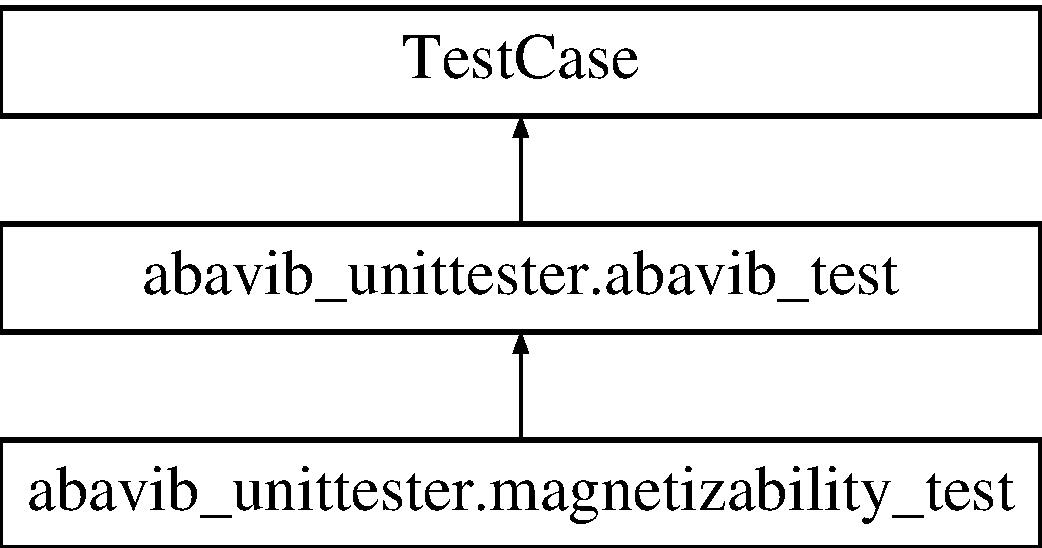
\includegraphics[height=3.000000cm]{classabavib__unittester_1_1magnetizability__test}
\end{center}
\end{figure}
\subsection*{Public Member Functions}
\begin{DoxyCompactItemize}
\item 
\hypertarget{classabavib__unittester_1_1magnetizability__test_ac27a40fddb70bda0fff7a000b72ba660}{def {\bfseries set\+Up}}\label{classabavib__unittester_1_1magnetizability__test_ac27a40fddb70bda0fff7a000b72ba660}

\item 
\hypertarget{classabavib__unittester_1_1magnetizability__test_a17f3538512a48c42cfb41d1ad5bc0a24}{def {\bfseries test\+\_\+magnetizability\+\_\+corrections}}\label{classabavib__unittester_1_1magnetizability__test_a17f3538512a48c42cfb41d1ad5bc0a24}

\item 
\hypertarget{classabavib__unittester_1_1magnetizability__test_a2bd0ab95861f7e8a15586626abd3183b}{def {\bfseries test\+\_\+magnetizability\+\_\+values}}\label{classabavib__unittester_1_1magnetizability__test_a2bd0ab95861f7e8a15586626abd3183b}

\end{DoxyCompactItemize}
\subsection*{Public Attributes}
\begin{DoxyCompactItemize}
\item 
\hypertarget{classabavib__unittester_1_1magnetizability__test_af5a150d0b494c0573ea280d2ee6dc533}{{\bfseries molecule}}\label{classabavib__unittester_1_1magnetizability__test_af5a150d0b494c0573ea280d2ee6dc533}

\item 
\hypertarget{classabavib__unittester_1_1magnetizability__test_abd3b2d980cce517777d8e5b15b994d9f}{{\bfseries eig}}\label{classabavib__unittester_1_1magnetizability__test_abd3b2d980cce517777d8e5b15b994d9f}

\item 
\hypertarget{classabavib__unittester_1_1magnetizability__test_af66fe08f778c2e7e02c1f0adb8da9636}{{\bfseries corrected\+\_\+values}}\label{classabavib__unittester_1_1magnetizability__test_af66fe08f778c2e7e02c1f0adb8da9636}

\item 
\hypertarget{classabavib__unittester_1_1magnetizability__test_a8b7916b50c9bbb7d6070b64a1f479c8a}{{\bfseries magnet}}\label{classabavib__unittester_1_1magnetizability__test_a8b7916b50c9bbb7d6070b64a1f479c8a}

\end{DoxyCompactItemize}
\subsection*{Additional Inherited Members}


The documentation for this class was generated from the following file\+:\begin{DoxyCompactItemize}
\item 
abavib\+\_\+unittester.\+py\end{DoxyCompactItemize}

\hypertarget{classabavib__unittester_1_1molecular__quadrupole__test}{\section{abavib\+\_\+unittester.\+molecular\+\_\+quadrupole\+\_\+test Class Reference}
\label{classabavib__unittester_1_1molecular__quadrupole__test}\index{abavib\+\_\+unittester.\+molecular\+\_\+quadrupole\+\_\+test@{abavib\+\_\+unittester.\+molecular\+\_\+quadrupole\+\_\+test}}
}
Inheritance diagram for abavib\+\_\+unittester.\+molecular\+\_\+quadrupole\+\_\+test\+:\begin{figure}[H]
\begin{center}
\leavevmode
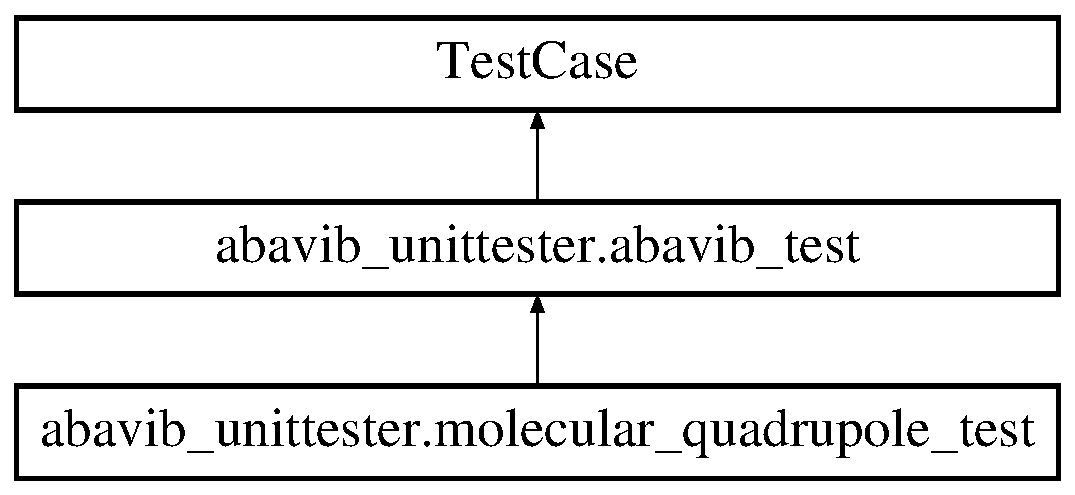
\includegraphics[height=3.000000cm]{classabavib__unittester_1_1molecular__quadrupole__test}
\end{center}
\end{figure}
\subsection*{Additional Inherited Members}


The documentation for this class was generated from the following file\+:\begin{DoxyCompactItemize}
\item 
abavib\+\_\+unittester.\+py\end{DoxyCompactItemize}

\hypertarget{classMolecule_1_1Molecule}{\section{Molecule.\+Molecule Class Reference}
\label{classMolecule_1_1Molecule}\index{Molecule.\+Molecule@{Molecule.\+Molecule}}
}
\subsection*{Public Member Functions}
\begin{DoxyCompactItemize}
\item 
\hypertarget{classMolecule_1_1Molecule_ac0ae55d23c730c26778fcfcc8e6cf143}{def {\bfseries \+\_\+\+\_\+init\+\_\+\+\_\+}}\label{classMolecule_1_1Molecule_ac0ae55d23c730c26778fcfcc8e6cf143}

\item 
def \hyperlink{classMolecule_1_1Molecule_a1ca29d097bb318928b097b1d7564346c}{get\+\_\+input\+\_\+name}
\item 
def \hyperlink{classMolecule_1_1Molecule_ad58fc49bdf93f6091533da4379a4bd86}{get\+\_\+output\+\_\+name}
\item 
def \hyperlink{classMolecule_1_1Molecule_ae6361f06aa090068ac2a51ccaf111a83}{get\+\_\+molecule\+\_\+input\+\_\+name}
\item 
def \hyperlink{classMolecule_1_1Molecule_a6a7ff9badbfe13eebd8047534bc049e6}{get\+\_\+cubic\+\_\+force\+\_\+field\+\_\+name}
\item 
def \hyperlink{classMolecule_1_1Molecule_aee1fe2aec71cb23b0dee8d8c0a07fbab}{get\+\_\+coordinates}
\item 
def \hyperlink{classMolecule_1_1Molecule_aa6c7a0fcbad7e948ab641ef01bfb6cff}{get\+\_\+number\+\_\+of\+\_\+normal\+\_\+modes}
\item 
def \hyperlink{classMolecule_1_1Molecule_a83e5685046b943d85007f3927fa6f45a}{get\+\_\+hessian}
\item 
def \hyperlink{classMolecule_1_1Molecule_a09c7bf3049234e8d4ecfffd0fbd5abc0}{hessian\+\_\+trans\+\_\+rot}
\item 
def \hyperlink{classMolecule_1_1Molecule_ac1ba969132f7988a5c03662d76d57235}{mass\+\_\+hessian}
\item 
def \hyperlink{classMolecule_1_1Molecule_a1d7291d2fd3f839f97507ad6c5acccbd}{masswt\+\_\+hessian}
\item 
def \hyperlink{classMolecule_1_1Molecule_a73503fd04984fa483a54032a919c4426}{diagonalize}
\item 
def \hyperlink{classMolecule_1_1Molecule_a121643aff37481b5182345ef95bc22b2}{to\+\_\+normal\+\_\+coordinates\+\_\+1\+D}
\item 
\hypertarget{classMolecule_1_1Molecule_a6657066ee4dd2db2762ef9f05b7b2cf0}{def {\bfseries to\+\_\+normal\+\_\+coordinates\+\_\+2\+D}}\label{classMolecule_1_1Molecule_a6657066ee4dd2db2762ef9f05b7b2cf0}

\item 
def \hyperlink{classMolecule_1_1Molecule_ae1292d157a94d00e99952e89ead7b2e7}{to\+\_\+normal\+\_\+coordinates\+\_\+3\+D}
\item 
def \hyperlink{classMolecule_1_1Molecule_af787ecd17f7d951af4864b6385bdb53d}{to\+\_\+normal\+\_\+coordinates\+\_\+4\+D}
\item 
def \hyperlink{classMolecule_1_1Molecule_af702cb533e33ab267e8a22298cf931bd}{get\+\_\+effective\+\_\+geometry}
\item 
def \hyperlink{classMolecule_1_1Molecule_a288f39b8931acfcb66efe859d1536adb}{effective\+\_\+geometry\+\_\+norm}
\end{DoxyCompactItemize}
\subsection*{Public Attributes}
\begin{DoxyCompactItemize}
\item 
\hypertarget{classMolecule_1_1Molecule_a9630d58089d0904bb73bfe8c14e65bcf}{{\bfseries name}}\label{classMolecule_1_1Molecule_a9630d58089d0904bb73bfe8c14e65bcf}

\item 
\hypertarget{classMolecule_1_1Molecule_adf9f60d1637552bb073c1175406c301b}{{\bfseries input\+\_\+name}}\label{classMolecule_1_1Molecule_adf9f60d1637552bb073c1175406c301b}

\item 
\hypertarget{classMolecule_1_1Molecule_a19339684751d377556d2527265b1d37c}{{\bfseries linear}}\label{classMolecule_1_1Molecule_a19339684751d377556d2527265b1d37c}

\item 
\hypertarget{classMolecule_1_1Molecule_a8aeb01cccf5091e6f1876c68722b23d4}{{\bfseries n\+\_\+atoms}}\label{classMolecule_1_1Molecule_a8aeb01cccf5091e6f1876c68722b23d4}

\item 
\hypertarget{classMolecule_1_1Molecule_a5cfd1fc24a27e949f91313c332e49f74}{{\bfseries coordinates}}\label{classMolecule_1_1Molecule_a5cfd1fc24a27e949f91313c332e49f74}

\item 
\hypertarget{classMolecule_1_1Molecule_a5f5a0fbf22fb70468754a86a41cbbdf5}{{\bfseries atom\+\_\+list}}\label{classMolecule_1_1Molecule_a5f5a0fbf22fb70468754a86a41cbbdf5}

\item 
\hypertarget{classMolecule_1_1Molecule_a950a7883f31a208890633dd7eb74b27b}{{\bfseries n\+\_\+coordinates}}\label{classMolecule_1_1Molecule_a950a7883f31a208890633dd7eb74b27b}

\item 
\hypertarget{classMolecule_1_1Molecule_a6865052d8d0d2c1de5d4451cba85b743}{{\bfseries number\+\_\+of\+\_\+normal\+\_\+modes}}\label{classMolecule_1_1Molecule_a6865052d8d0d2c1de5d4451cba85b743}

\item 
\hypertarget{classMolecule_1_1Molecule_a07c391c72fd76f841d3b40171c4003fc}{{\bfseries hessian}}\label{classMolecule_1_1Molecule_a07c391c72fd76f841d3b40171c4003fc}

\item 
\hypertarget{classMolecule_1_1Molecule_a98b6ad60e77cdb3aca3962ce9f5c11ac}{{\bfseries eigenvectors\+\_\+full}}\label{classMolecule_1_1Molecule_a98b6ad60e77cdb3aca3962ce9f5c11ac}

\item 
\hypertarget{classMolecule_1_1Molecule_a6b124c1491f81729260fa407ceb2cfae}{{\bfseries cff\+\_\+norm}}\label{classMolecule_1_1Molecule_a6b124c1491f81729260fa407ceb2cfae}

\item 
\hypertarget{classMolecule_1_1Molecule_a4c0104a2109e6ae8811cddf98000c195}{{\bfseries effective\+\_\+geometry}}\label{classMolecule_1_1Molecule_a4c0104a2109e6ae8811cddf98000c195}

\end{DoxyCompactItemize}


\subsection{Member Function Documentation}
\hypertarget{classMolecule_1_1Molecule_a73503fd04984fa483a54032a919c4426}{\index{Molecule\+::\+Molecule@{Molecule\+::\+Molecule}!diagonalize@{diagonalize}}
\index{diagonalize@{diagonalize}!Molecule\+::\+Molecule@{Molecule\+::\+Molecule}}
\subsubsection[{diagonalize}]{\setlength{\rightskip}{0pt plus 5cm}def Molecule.\+Molecule.\+diagonalize (
\begin{DoxyParamCaption}
\item[{}]{self, }
\item[{}]{hessian}
\end{DoxyParamCaption}
)}}\label{classMolecule_1_1Molecule_a73503fd04984fa483a54032a919c4426}
\begin{DoxyVerb}Computes the normal coordinates, eigenvalues and fundamental 
frequencies of the molecule. 
hessian: The hessian of the molecule as an np.array
num_atoms_list: A list of the how many of each atoms type there are
charge list: A list over the charges of the atoms in the molecle
coordinates: The cartessian coordinates of the molecule as an np.array
n_atoms: The number of atoms composing the molecule as an int
masses: The masses of the atoms in a molecule along the diagonal of
an np.array
returns: The non-zero eigenvalues of the molecule as an np.array
 The normal coordinates of the molecule, ie. the eigenvectors
 corresponding the non-zero eigevalues as an np.array
 The fundalmental frequencies of the molecule as an np.array
 All the eigenvectos of the molecules, both the ones 
 corresponding the zero and non-zero eigenvalues as an np.array
\end{DoxyVerb}
 \hypertarget{classMolecule_1_1Molecule_a288f39b8931acfcb66efe859d1536adb}{\index{Molecule\+::\+Molecule@{Molecule\+::\+Molecule}!effective\+\_\+geometry\+\_\+norm@{effective\+\_\+geometry\+\_\+norm}}
\index{effective\+\_\+geometry\+\_\+norm@{effective\+\_\+geometry\+\_\+norm}!Molecule\+::\+Molecule@{Molecule\+::\+Molecule}}
\subsubsection[{effective\+\_\+geometry\+\_\+norm}]{\setlength{\rightskip}{0pt plus 5cm}def Molecule.\+Molecule.\+effective\+\_\+geometry\+\_\+norm (
\begin{DoxyParamCaption}
\item[{}]{self, }
\item[{}]{cff\+\_\+norm}
\end{DoxyParamCaption}
)}}\label{classMolecule_1_1Molecule_a288f39b8931acfcb66efe859d1536adb}
\begin{DoxyVerb}Computes the effective geometry of a molecule.

cff_norm: The cubic force field of the molecule in normal coordinates
  as an np.array
frequencies: The fundamental frequencies of the molecule as an np.array
n_atoms: The number of atoms constituting the molecule as an int
return: The effective geometry in normal coordinates as an np.arrays
\end{DoxyVerb}
 \hypertarget{classMolecule_1_1Molecule_aee1fe2aec71cb23b0dee8d8c0a07fbab}{\index{Molecule\+::\+Molecule@{Molecule\+::\+Molecule}!get\+\_\+coordinates@{get\+\_\+coordinates}}
\index{get\+\_\+coordinates@{get\+\_\+coordinates}!Molecule\+::\+Molecule@{Molecule\+::\+Molecule}}
\subsubsection[{get\+\_\+coordinates}]{\setlength{\rightskip}{0pt plus 5cm}def Molecule.\+Molecule.\+get\+\_\+coordinates (
\begin{DoxyParamCaption}
\item[{}]{self}
\end{DoxyParamCaption}
)}}\label{classMolecule_1_1Molecule_aee1fe2aec71cb23b0dee8d8c0a07fbab}
\begin{DoxyVerb}Returns the number of coordinates of the molecule\end{DoxyVerb}
 \hypertarget{classMolecule_1_1Molecule_a6a7ff9badbfe13eebd8047534bc049e6}{\index{Molecule\+::\+Molecule@{Molecule\+::\+Molecule}!get\+\_\+cubic\+\_\+force\+\_\+field\+\_\+name@{get\+\_\+cubic\+\_\+force\+\_\+field\+\_\+name}}
\index{get\+\_\+cubic\+\_\+force\+\_\+field\+\_\+name@{get\+\_\+cubic\+\_\+force\+\_\+field\+\_\+name}!Molecule\+::\+Molecule@{Molecule\+::\+Molecule}}
\subsubsection[{get\+\_\+cubic\+\_\+force\+\_\+field\+\_\+name}]{\setlength{\rightskip}{0pt plus 5cm}def Molecule.\+Molecule.\+get\+\_\+cubic\+\_\+force\+\_\+field\+\_\+name (
\begin{DoxyParamCaption}
\item[{}]{self}
\end{DoxyParamCaption}
)}}\label{classMolecule_1_1Molecule_a6a7ff9badbfe13eebd8047534bc049e6}
\begin{DoxyVerb}Returns the  name of the file containing the cubic force field
 of the molecule\end{DoxyVerb}
 \hypertarget{classMolecule_1_1Molecule_af702cb533e33ab267e8a22298cf931bd}{\index{Molecule\+::\+Molecule@{Molecule\+::\+Molecule}!get\+\_\+effective\+\_\+geometry@{get\+\_\+effective\+\_\+geometry}}
\index{get\+\_\+effective\+\_\+geometry@{get\+\_\+effective\+\_\+geometry}!Molecule\+::\+Molecule@{Molecule\+::\+Molecule}}
\subsubsection[{get\+\_\+effective\+\_\+geometry}]{\setlength{\rightskip}{0pt plus 5cm}def Molecule.\+Molecule.\+get\+\_\+effective\+\_\+geometry (
\begin{DoxyParamCaption}
\item[{}]{self}
\end{DoxyParamCaption}
)}}\label{classMolecule_1_1Molecule_af702cb533e33ab267e8a22298cf931bd}
\begin{DoxyVerb}Converts normal coordinates into cartessian coordinates.

normal coordinates: The normal coordinates of which are to be converted
n_atoms: The number of atoms constituting the molecule as an int
eigvec: The eigenvectors of the molecule corresponging to the non
zero eigenvalues, can be attained for fundamental_freq() (np.array)
returns: cartessian coordinates as an np.array.
\end{DoxyVerb}
 \hypertarget{classMolecule_1_1Molecule_a83e5685046b943d85007f3927fa6f45a}{\index{Molecule\+::\+Molecule@{Molecule\+::\+Molecule}!get\+\_\+hessian@{get\+\_\+hessian}}
\index{get\+\_\+hessian@{get\+\_\+hessian}!Molecule\+::\+Molecule@{Molecule\+::\+Molecule}}
\subsubsection[{get\+\_\+hessian}]{\setlength{\rightskip}{0pt plus 5cm}def Molecule.\+Molecule.\+get\+\_\+hessian (
\begin{DoxyParamCaption}
\item[{}]{self}
\end{DoxyParamCaption}
)}}\label{classMolecule_1_1Molecule_a83e5685046b943d85007f3927fa6f45a}
\begin{DoxyVerb}Returns the hessian of the molecule\end{DoxyVerb}
 \hypertarget{classMolecule_1_1Molecule_a1ca29d097bb318928b097b1d7564346c}{\index{Molecule\+::\+Molecule@{Molecule\+::\+Molecule}!get\+\_\+input\+\_\+name@{get\+\_\+input\+\_\+name}}
\index{get\+\_\+input\+\_\+name@{get\+\_\+input\+\_\+name}!Molecule\+::\+Molecule@{Molecule\+::\+Molecule}}
\subsubsection[{get\+\_\+input\+\_\+name}]{\setlength{\rightskip}{0pt plus 5cm}def Molecule.\+Molecule.\+get\+\_\+input\+\_\+name (
\begin{DoxyParamCaption}
\item[{}]{self}
\end{DoxyParamCaption}
)}}\label{classMolecule_1_1Molecule_a1ca29d097bb318928b097b1d7564346c}
\begin{DoxyVerb}Returns the name of the directory the input files are to be 
read are found.\end{DoxyVerb}
 \hypertarget{classMolecule_1_1Molecule_ae6361f06aa090068ac2a51ccaf111a83}{\index{Molecule\+::\+Molecule@{Molecule\+::\+Molecule}!get\+\_\+molecule\+\_\+input\+\_\+name@{get\+\_\+molecule\+\_\+input\+\_\+name}}
\index{get\+\_\+molecule\+\_\+input\+\_\+name@{get\+\_\+molecule\+\_\+input\+\_\+name}!Molecule\+::\+Molecule@{Molecule\+::\+Molecule}}
\subsubsection[{get\+\_\+molecule\+\_\+input\+\_\+name}]{\setlength{\rightskip}{0pt plus 5cm}def Molecule.\+Molecule.\+get\+\_\+molecule\+\_\+input\+\_\+name (
\begin{DoxyParamCaption}
\item[{}]{self}
\end{DoxyParamCaption}
)}}\label{classMolecule_1_1Molecule_ae6361f06aa090068ac2a51ccaf111a83}
\begin{DoxyVerb}Returns the  name of the file containing the geometry of the
 molecule in cartessian coordinates\end{DoxyVerb}
 \hypertarget{classMolecule_1_1Molecule_aa6c7a0fcbad7e948ab641ef01bfb6cff}{\index{Molecule\+::\+Molecule@{Molecule\+::\+Molecule}!get\+\_\+number\+\_\+of\+\_\+normal\+\_\+modes@{get\+\_\+number\+\_\+of\+\_\+normal\+\_\+modes}}
\index{get\+\_\+number\+\_\+of\+\_\+normal\+\_\+modes@{get\+\_\+number\+\_\+of\+\_\+normal\+\_\+modes}!Molecule\+::\+Molecule@{Molecule\+::\+Molecule}}
\subsubsection[{get\+\_\+number\+\_\+of\+\_\+normal\+\_\+modes}]{\setlength{\rightskip}{0pt plus 5cm}def Molecule.\+Molecule.\+get\+\_\+number\+\_\+of\+\_\+normal\+\_\+modes (
\begin{DoxyParamCaption}
\item[{}]{self}
\end{DoxyParamCaption}
)}}\label{classMolecule_1_1Molecule_aa6c7a0fcbad7e948ab641ef01bfb6cff}
\begin{DoxyVerb}Returns the number of normal modes of the molecule\end{DoxyVerb}
 \hypertarget{classMolecule_1_1Molecule_ad58fc49bdf93f6091533da4379a4bd86}{\index{Molecule\+::\+Molecule@{Molecule\+::\+Molecule}!get\+\_\+output\+\_\+name@{get\+\_\+output\+\_\+name}}
\index{get\+\_\+output\+\_\+name@{get\+\_\+output\+\_\+name}!Molecule\+::\+Molecule@{Molecule\+::\+Molecule}}
\subsubsection[{get\+\_\+output\+\_\+name}]{\setlength{\rightskip}{0pt plus 5cm}def Molecule.\+Molecule.\+get\+\_\+output\+\_\+name (
\begin{DoxyParamCaption}
\item[{}]{self}
\end{DoxyParamCaption}
)}}\label{classMolecule_1_1Molecule_ad58fc49bdf93f6091533da4379a4bd86}
\begin{DoxyVerb}Returns the name of the directory the output information is to
be saved in.\end{DoxyVerb}
 \hypertarget{classMolecule_1_1Molecule_a09c7bf3049234e8d4ecfffd0fbd5abc0}{\index{Molecule\+::\+Molecule@{Molecule\+::\+Molecule}!hessian\+\_\+trans\+\_\+rot@{hessian\+\_\+trans\+\_\+rot}}
\index{hessian\+\_\+trans\+\_\+rot@{hessian\+\_\+trans\+\_\+rot}!Molecule\+::\+Molecule@{Molecule\+::\+Molecule}}
\subsubsection[{hessian\+\_\+trans\+\_\+rot}]{\setlength{\rightskip}{0pt plus 5cm}def Molecule.\+Molecule.\+hessian\+\_\+trans\+\_\+rot (
\begin{DoxyParamCaption}
\item[{}]{self, }
\item[{}]{hessian, }
\item[{}]{cart\+\_\+coord, }
\item[{}]{nr\+\_\+normal\+\_\+modes, }
\item[{}]{n\+\_\+atoms}
\end{DoxyParamCaption}
)}}\label{classMolecule_1_1Molecule_a09c7bf3049234e8d4ecfffd0fbd5abc0}
\begin{DoxyVerb}Projects the hessian of the molecule so that it can be used to 
determine the normal coordinates of the molecule. This projected
hessian is referred to as the analystical hessian in DALTON

hessian: The hessian of the molecule as an np.array
nr_normal_modes: The number of normal modes of the molecule as an 
     int
n_atoms: The number of atoms the molecule consists of
return: The projected hessian as a 2 dimensional matrix                  
\end{DoxyVerb}
 \hypertarget{classMolecule_1_1Molecule_ac1ba969132f7988a5c03662d76d57235}{\index{Molecule\+::\+Molecule@{Molecule\+::\+Molecule}!mass\+\_\+hessian@{mass\+\_\+hessian}}
\index{mass\+\_\+hessian@{mass\+\_\+hessian}!Molecule\+::\+Molecule@{Molecule\+::\+Molecule}}
\subsubsection[{mass\+\_\+hessian}]{\setlength{\rightskip}{0pt plus 5cm}def Molecule.\+Molecule.\+mass\+\_\+hessian (
\begin{DoxyParamCaption}
\item[{}]{self, }
\item[{}]{masses}
\end{DoxyParamCaption}
)}}\label{classMolecule_1_1Molecule_ac1ba969132f7988a5c03662d76d57235}
\begin{DoxyVerb}Creates an np.array where the masses of the different atoms in
the molecule are placed at the diagonal. This is a help function
used to make a mass weighted hessian. 
masses: The masses of the atoms in the molecule, can be recieved
from the read_molecule() function.
returns: The masses alond the diagonal of a 2 dimensional np.array
\end{DoxyVerb}
 \hypertarget{classMolecule_1_1Molecule_a1d7291d2fd3f839f97507ad6c5acccbd}{\index{Molecule\+::\+Molecule@{Molecule\+::\+Molecule}!masswt\+\_\+hessian@{masswt\+\_\+hessian}}
\index{masswt\+\_\+hessian@{masswt\+\_\+hessian}!Molecule\+::\+Molecule@{Molecule\+::\+Molecule}}
\subsubsection[{masswt\+\_\+hessian}]{\setlength{\rightskip}{0pt plus 5cm}def Molecule.\+Molecule.\+masswt\+\_\+hessian (
\begin{DoxyParamCaption}
\item[{}]{self, }
\item[{}]{num\+\_\+atoms\+\_\+list, }
\item[{}]{charge\+\_\+list}
\end{DoxyParamCaption}
)}}\label{classMolecule_1_1Molecule_a1d7291d2fd3f839f97507ad6c5acccbd}
\begin{DoxyVerb}Converts the hessian into the mass weighted hessian
num_atoms_list: A list of the number of atoms of each type
charge list: A list of the charges of each atom 
returns the mass weighted hessian (np.array)\end{DoxyVerb}
 \hypertarget{classMolecule_1_1Molecule_a121643aff37481b5182345ef95bc22b2}{\index{Molecule\+::\+Molecule@{Molecule\+::\+Molecule}!to\+\_\+normal\+\_\+coordinates\+\_\+1\+D@{to\+\_\+normal\+\_\+coordinates\+\_\+1\+D}}
\index{to\+\_\+normal\+\_\+coordinates\+\_\+1\+D@{to\+\_\+normal\+\_\+coordinates\+\_\+1\+D}!Molecule\+::\+Molecule@{Molecule\+::\+Molecule}}
\subsubsection[{to\+\_\+normal\+\_\+coordinates\+\_\+1\+D}]{\setlength{\rightskip}{0pt plus 5cm}def Molecule.\+Molecule.\+to\+\_\+normal\+\_\+coordinates\+\_\+1\+D (
\begin{DoxyParamCaption}
\item[{}]{self}
\end{DoxyParamCaption}
)}}\label{classMolecule_1_1Molecule_a121643aff37481b5182345ef95bc22b2}
\begin{DoxyVerb}Converts 1D np.arrays from cartessian to normal coordinates, an 
example of this is the dipole moment gradients

gradient = A 1 dimensional np.array 
returns: the 1 dimensional np.array in normal coordinates
\end{DoxyVerb}
 \hypertarget{classMolecule_1_1Molecule_ae1292d157a94d00e99952e89ead7b2e7}{\index{Molecule\+::\+Molecule@{Molecule\+::\+Molecule}!to\+\_\+normal\+\_\+coordinates\+\_\+3\+D@{to\+\_\+normal\+\_\+coordinates\+\_\+3\+D}}
\index{to\+\_\+normal\+\_\+coordinates\+\_\+3\+D@{to\+\_\+normal\+\_\+coordinates\+\_\+3\+D}!Molecule\+::\+Molecule@{Molecule\+::\+Molecule}}
\subsubsection[{to\+\_\+normal\+\_\+coordinates\+\_\+3\+D}]{\setlength{\rightskip}{0pt plus 5cm}def Molecule.\+Molecule.\+to\+\_\+normal\+\_\+coordinates\+\_\+3\+D (
\begin{DoxyParamCaption}
\item[{}]{self, }
\item[{}]{cubic\+\_\+force\+\_\+field}
\end{DoxyParamCaption}
)}}\label{classMolecule_1_1Molecule_ae1292d157a94d00e99952e89ead7b2e7}
\begin{DoxyVerb}Converts a cubic force field represented by cartessian coordinates
into a cubic force field represented by normal coordinates

cubic_force_field: A 3 dimenesional np.array of the cubic force field
           represented in cartessian coordinates
self.eigenvectors_full: The eigenvectors of the molecule corresponding to the non-
zero eigenvalues, can be attained for fundamental_freq() (np.array)
n_atoms: The number of atoms constituting the molecule as an int
returns: The cubic force field in normal coordinates (3D np.array)
\end{DoxyVerb}
 \hypertarget{classMolecule_1_1Molecule_af787ecd17f7d951af4864b6385bdb53d}{\index{Molecule\+::\+Molecule@{Molecule\+::\+Molecule}!to\+\_\+normal\+\_\+coordinates\+\_\+4\+D@{to\+\_\+normal\+\_\+coordinates\+\_\+4\+D}}
\index{to\+\_\+normal\+\_\+coordinates\+\_\+4\+D@{to\+\_\+normal\+\_\+coordinates\+\_\+4\+D}!Molecule\+::\+Molecule@{Molecule\+::\+Molecule}}
\subsubsection[{to\+\_\+normal\+\_\+coordinates\+\_\+4\+D}]{\setlength{\rightskip}{0pt plus 5cm}def Molecule.\+Molecule.\+to\+\_\+normal\+\_\+coordinates\+\_\+4\+D (
\begin{DoxyParamCaption}
\item[{}]{self, }
\item[{}]{quartic\+\_\+force\+\_\+field}
\end{DoxyParamCaption}
)}}\label{classMolecule_1_1Molecule_af787ecd17f7d951af4864b6385bdb53d}
\begin{DoxyVerb}Converts a quartic force field represented by cartessina coordinates
into a quartic force field represented by normal coordinates

quartic_force_field: A 4 dimenesional np.array of the quartic force field
           represented in cartessian coordinates
self.eigenvectors_full: The eigenvectors of the molecule corresponding to the non-
zero eigenvalues, can be attained from fundamental_freq() (np.array)
n_atoms: The number of atoms constituting the molecule as an int
returns: The quartic force field in normal coordinates ( 4d np.array)
\end{DoxyVerb}
 

The documentation for this class was generated from the following file\+:\begin{DoxyCompactItemize}
\item 
Molecule.\+py\end{DoxyCompactItemize}

\hypertarget{classabavib__unittester_1_1nuclear__quadrupole__test}{\section{abavib\+\_\+unittester.\+nuclear\+\_\+quadrupole\+\_\+test Class Reference}
\label{classabavib__unittester_1_1nuclear__quadrupole__test}\index{abavib\+\_\+unittester.\+nuclear\+\_\+quadrupole\+\_\+test@{abavib\+\_\+unittester.\+nuclear\+\_\+quadrupole\+\_\+test}}
}
Inheritance diagram for abavib\+\_\+unittester.\+nuclear\+\_\+quadrupole\+\_\+test\+:\begin{figure}[H]
\begin{center}
\leavevmode
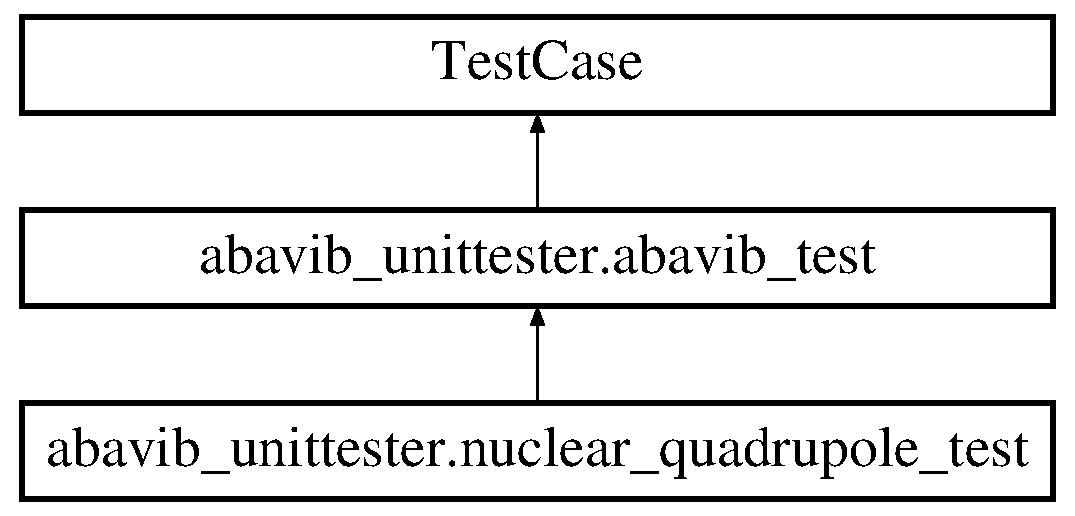
\includegraphics[height=3.000000cm]{classabavib__unittester_1_1nuclear__quadrupole__test}
\end{center}
\end{figure}
\subsection*{Additional Inherited Members}


The documentation for this class was generated from the following file\+:\begin{DoxyCompactItemize}
\item 
abavib\+\_\+unittester.\+py\end{DoxyCompactItemize}

\hypertarget{classchiral__tester_1_1optical__rotation__test}{\section{chiral\+\_\+tester.\+optical\+\_\+rotation\+\_\+test Class Reference}
\label{classchiral__tester_1_1optical__rotation__test}\index{chiral\+\_\+tester.\+optical\+\_\+rotation\+\_\+test@{chiral\+\_\+tester.\+optical\+\_\+rotation\+\_\+test}}
}
Inheritance diagram for chiral\+\_\+tester.\+optical\+\_\+rotation\+\_\+test\+:\begin{figure}[H]
\begin{center}
\leavevmode
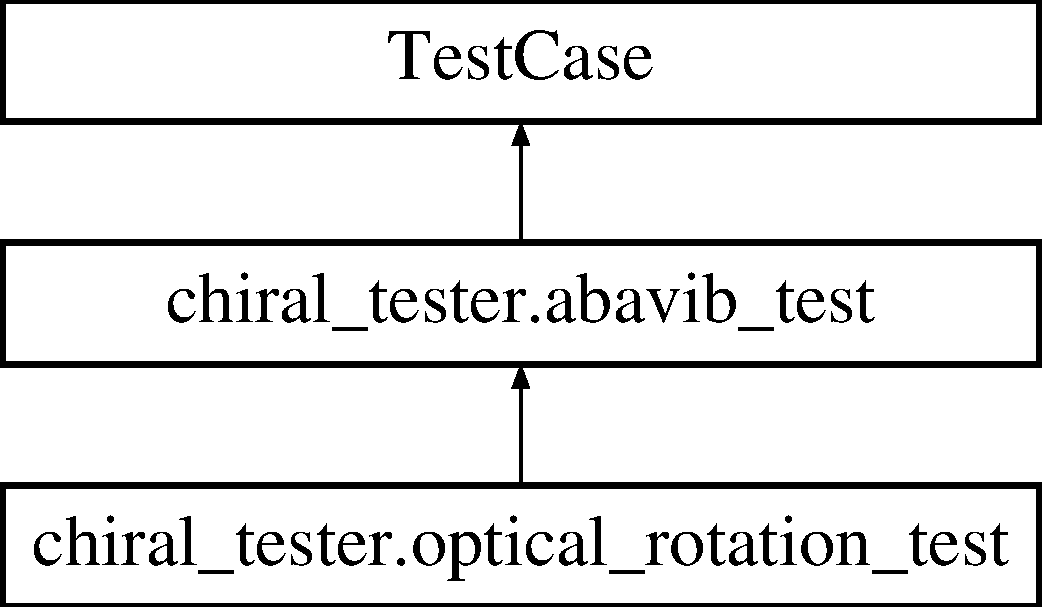
\includegraphics[height=3.000000cm]{classchiral__tester_1_1optical__rotation__test}
\end{center}
\end{figure}
\subsection*{Public Member Functions}
\begin{DoxyCompactItemize}
\item 
\hypertarget{classchiral__tester_1_1optical__rotation__test_a6b6e93715f34310786f38ab4f44e5e70}{def {\bfseries set\+Up}}\label{classchiral__tester_1_1optical__rotation__test_a6b6e93715f34310786f38ab4f44e5e70}

\item 
\hypertarget{classchiral__tester_1_1optical__rotation__test_af59471763111452bf72cd62425062ee0}{def {\bfseries test\+\_\+optical\+\_\+rotation\+\_\+corrections}}\label{classchiral__tester_1_1optical__rotation__test_af59471763111452bf72cd62425062ee0}

\item 
\hypertarget{classchiral__tester_1_1optical__rotation__test_a1a3bab35383a0489e43d32a212776b74}{def {\bfseries test\+\_\+optical\+\_\+rotation\+\_\+values}}\label{classchiral__tester_1_1optical__rotation__test_a1a3bab35383a0489e43d32a212776b74}

\end{DoxyCompactItemize}
\subsection*{Public Attributes}
\begin{DoxyCompactItemize}
\item 
\hypertarget{classchiral__tester_1_1optical__rotation__test_a9309df9124146940a88535e5c5d29d48}{{\bfseries corrected\+\_\+values}}\label{classchiral__tester_1_1optical__rotation__test_a9309df9124146940a88535e5c5d29d48}

\item 
\hypertarget{classchiral__tester_1_1optical__rotation__test_a92458035f0e9d56eda4a80820b32324b}{{\bfseries optrot}}\label{classchiral__tester_1_1optical__rotation__test_a92458035f0e9d56eda4a80820b32324b}

\end{DoxyCompactItemize}
\subsection*{Additional Inherited Members}


The documentation for this class was generated from the following file\+:\begin{DoxyCompactItemize}
\item 
chiral\+\_\+tester.\+py\end{DoxyCompactItemize}

\hypertarget{classPropertyclasses_1_1Polarizability}{\section{Propertyclasses.\+Polarizability Class Reference}
\label{classPropertyclasses_1_1Polarizability}\index{Propertyclasses.\+Polarizability@{Propertyclasses.\+Polarizability}}
}
\subsection*{Public Member Functions}
\begin{DoxyCompactItemize}
\item 
def \hyperlink{classPropertyclasses_1_1Polarizability_a9101b6a148a5ea640fc9f802b37881fb}{\+\_\+\+\_\+call\+\_\+\+\_\+}
\end{DoxyCompactItemize}


\subsection{Member Function Documentation}
\hypertarget{classPropertyclasses_1_1Polarizability_a9101b6a148a5ea640fc9f802b37881fb}{\index{Propertyclasses\+::\+Polarizability@{Propertyclasses\+::\+Polarizability}!\+\_\+\+\_\+call\+\_\+\+\_\+@{\+\_\+\+\_\+call\+\_\+\+\_\+}}
\index{\+\_\+\+\_\+call\+\_\+\+\_\+@{\+\_\+\+\_\+call\+\_\+\+\_\+}!Propertyclasses\+::\+Polarizability@{Propertyclasses\+::\+Polarizability}}
\subsubsection[{\+\_\+\+\_\+call\+\_\+\+\_\+}]{\setlength{\rightskip}{0pt plus 5cm}def Propertyclasses.\+Polarizability.\+\_\+\+\_\+call\+\_\+\+\_\+ (
\begin{DoxyParamCaption}
{}
\end{DoxyParamCaption}
)}}\label{classPropertyclasses_1_1Polarizability_a9101b6a148a5ea640fc9f802b37881fb}
\begin{DoxyVerb}Computes polarizability corrections and adds the corrections
to the original value of the polarizabilty.
property_type: The name of the first tensor property, used when
       writing to file
pre_property: The second derivative of the property
Uncorrected property: The property before the corrections
nm: Number of normal modes for of the molecule
eig: The non-zero eigenvalues of the molecules hessian
polar: If the molecule is polar or not, as a bollean.
returns: The corrections to the property, the corrected property as 
 np.arrays\end{DoxyVerb}
 

The documentation for this class was generated from the following file\+:\begin{DoxyCompactItemize}
\item 
Propertyclasses.\+py\end{DoxyCompactItemize}

\hypertarget{classabavib__unittester_1_1polarizability__test}{\section{abavib\+\_\+unittester.\+polarizability\+\_\+test Class Reference}
\label{classabavib__unittester_1_1polarizability__test}\index{abavib\+\_\+unittester.\+polarizability\+\_\+test@{abavib\+\_\+unittester.\+polarizability\+\_\+test}}
}
Inheritance diagram for abavib\+\_\+unittester.\+polarizability\+\_\+test\+:\begin{figure}[H]
\begin{center}
\leavevmode
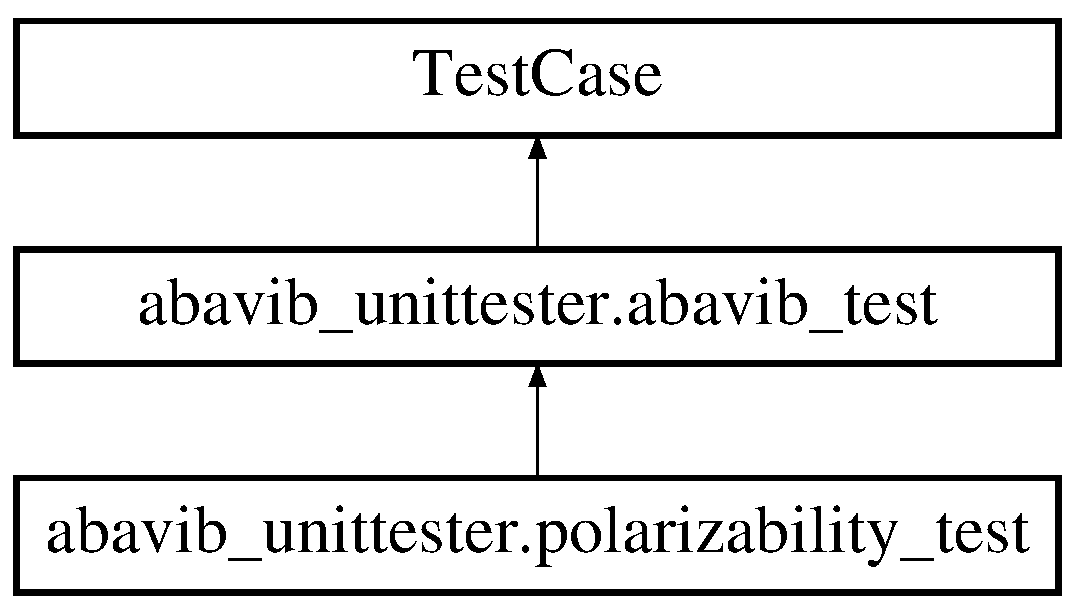
\includegraphics[height=3.000000cm]{classabavib__unittester_1_1polarizability__test}
\end{center}
\end{figure}
\subsection*{Public Member Functions}
\begin{DoxyCompactItemize}
\item 
\hypertarget{classabavib__unittester_1_1polarizability__test_aa5a23f608383c2742e092101a8cc3000}{def {\bfseries set\+Up}}\label{classabavib__unittester_1_1polarizability__test_aa5a23f608383c2742e092101a8cc3000}

\item 
\hypertarget{classabavib__unittester_1_1polarizability__test_aa03cd46336f00235226c5be6f18e7482}{def {\bfseries test\+\_\+polarizability\+\_\+corrections}}\label{classabavib__unittester_1_1polarizability__test_aa03cd46336f00235226c5be6f18e7482}

\item 
\hypertarget{classabavib__unittester_1_1polarizability__test_a5f0b7cc0e297040f881e80f81f050055}{def {\bfseries test\+\_\+polarizability\+\_\+values}}\label{classabavib__unittester_1_1polarizability__test_a5f0b7cc0e297040f881e80f81f050055}

\end{DoxyCompactItemize}
\subsection*{Public Attributes}
\begin{DoxyCompactItemize}
\item 
\hypertarget{classabavib__unittester_1_1polarizability__test_aed2bb9a607338be4fefece3f8dc656ec}{{\bfseries prop\+\_\+type}}\label{classabavib__unittester_1_1polarizability__test_aed2bb9a607338be4fefece3f8dc656ec}

\item 
\hypertarget{classabavib__unittester_1_1polarizability__test_a8b710465395086dc0021c69cfc5ffa72}{{\bfseries corrected\+\_\+values}}\label{classabavib__unittester_1_1polarizability__test_a8b710465395086dc0021c69cfc5ffa72}

\item 
\hypertarget{classabavib__unittester_1_1polarizability__test_a989c132876fa2dccdcd31084809f8baa}{{\bfseries polari}}\label{classabavib__unittester_1_1polarizability__test_a989c132876fa2dccdcd31084809f8baa}

\item 
\hypertarget{classabavib__unittester_1_1polarizability__test_a588b4edea8db1a49cb2e7098459ca04b}{{\bfseries molecule}}\label{classabavib__unittester_1_1polarizability__test_a588b4edea8db1a49cb2e7098459ca04b}

\end{DoxyCompactItemize}
\subsection*{Additional Inherited Members}


The documentation for this class was generated from the following file\+:\begin{DoxyCompactItemize}
\item 
abavib\+\_\+unittester.\+py\end{DoxyCompactItemize}

\hypertarget{classProperty_1_1Property}{\section{Property.\+Property Class Reference}
\label{classProperty_1_1Property}\index{Property.\+Property@{Property.\+Property}}
}
Inheritance diagram for Property.\+Property\+:\begin{figure}[H]
\begin{center}
\leavevmode
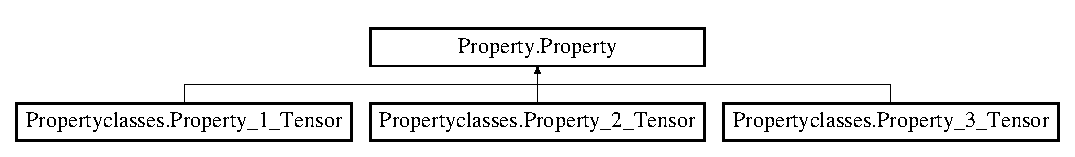
\includegraphics[height=1.666667cm]{classProperty_1_1Property}
\end{center}
\end{figure}
\subsection*{Public Member Functions}
\begin{DoxyCompactItemize}
\item 
\hypertarget{classProperty_1_1Property_a9a022528df4e8d4c6a7664826af48a54}{def {\bfseries \+\_\+\+\_\+init\+\_\+\+\_\+}}\label{classProperty_1_1Property_a9a022528df4e8d4c6a7664826af48a54}

\item 
def \hyperlink{classProperty_1_1Property_a45a72dc8487d8537c6d14cfed5663139}{\+\_\+\+\_\+call\+\_\+\+\_\+}
\item 
def \hyperlink{classProperty_1_1Property_ae98895c0fc4edb65ecc6f262a1d870da}{quartic\+\_\+precision}
\item 
def \hyperlink{classProperty_1_1Property_acbce93000fa76899a14184a1177f0560}{get\+\_\+quartic\+\_\+force\+\_\+field}
\item 
def \hyperlink{classProperty_1_1Property_a70bfec9e630a20db49fe05ef2ca58682}{write\+\_\+to\+\_\+file}
\end{DoxyCompactItemize}
\subsection*{Public Attributes}
\begin{DoxyCompactItemize}
\item 
\hypertarget{classProperty_1_1Property_a081689db7731edaf89f3d7a3e1f78680}{{\bfseries m\+\_\+e}}\label{classProperty_1_1Property_a081689db7731edaf89f3d7a3e1f78680}

\item 
\hypertarget{classProperty_1_1Property_a2b1de8d9b1024c2d09cccb837b8ba803}{{\bfseries prefactor}}\label{classProperty_1_1Property_a2b1de8d9b1024c2d09cccb837b8ba803}

\item 
\hypertarget{classProperty_1_1Property_a076e81d95a892945d0e96cd3e1618553}{{\bfseries molecule}}\label{classProperty_1_1Property_a076e81d95a892945d0e96cd3e1618553}

\item 
\hypertarget{classProperty_1_1Property_acc63967a91b7bbc8cf8e51f1fabd2910}{{\bfseries freq}}\label{classProperty_1_1Property_acc63967a91b7bbc8cf8e51f1fabd2910}

\end{DoxyCompactItemize}


\subsection{Detailed Description}
\begin{DoxyVerb}The superclass for calculating properties of a molecule\end{DoxyVerb}
 

\subsection{Member Function Documentation}
\hypertarget{classProperty_1_1Property_a45a72dc8487d8537c6d14cfed5663139}{\index{Property\+::\+Property@{Property\+::\+Property}!\+\_\+\+\_\+call\+\_\+\+\_\+@{\+\_\+\+\_\+call\+\_\+\+\_\+}}
\index{\+\_\+\+\_\+call\+\_\+\+\_\+@{\+\_\+\+\_\+call\+\_\+\+\_\+}!Property\+::\+Property@{Property\+::\+Property}}
\subsubsection[{\+\_\+\+\_\+call\+\_\+\+\_\+}]{\setlength{\rightskip}{0pt plus 5cm}def Property.\+Property.\+\_\+\+\_\+call\+\_\+\+\_\+ (
\begin{DoxyParamCaption}
{}
\end{DoxyParamCaption}
)}}\label{classProperty_1_1Property_a45a72dc8487d8537c6d14cfed5663139}
\begin{DoxyVerb}The superclass for the call function, raises a NotImplementedError.\end{DoxyVerb}
 \hypertarget{classProperty_1_1Property_acbce93000fa76899a14184a1177f0560}{\index{Property\+::\+Property@{Property\+::\+Property}!get\+\_\+quartic\+\_\+force\+\_\+field@{get\+\_\+quartic\+\_\+force\+\_\+field}}
\index{get\+\_\+quartic\+\_\+force\+\_\+field@{get\+\_\+quartic\+\_\+force\+\_\+field}!Property\+::\+Property@{Property\+::\+Property}}
\subsubsection[{get\+\_\+quartic\+\_\+force\+\_\+field}]{\setlength{\rightskip}{0pt plus 5cm}def Property.\+Property.\+get\+\_\+quartic\+\_\+force\+\_\+field (
\begin{DoxyParamCaption}
\item[{}]{self}
\end{DoxyParamCaption}
)}}\label{classProperty_1_1Property_acbce93000fa76899a14184a1177f0560}
\begin{DoxyVerb}Returns the quartic force field in cartessian coordinates as 
a 4D np.array\end{DoxyVerb}
 \hypertarget{classProperty_1_1Property_ae98895c0fc4edb65ecc6f262a1d870da}{\index{Property\+::\+Property@{Property\+::\+Property}!quartic\+\_\+precision@{quartic\+\_\+precision}}
\index{quartic\+\_\+precision@{quartic\+\_\+precision}!Property\+::\+Property@{Property\+::\+Property}}
\subsubsection[{quartic\+\_\+precision}]{\setlength{\rightskip}{0pt plus 5cm}def Property.\+Property.\+quartic\+\_\+precision (
\begin{DoxyParamCaption}
\item[{}]{cff\+\_\+norm, }
\item[{}]{qff\+\_\+norm, }
\item[{}]{prop\+\_\+deriv}
\end{DoxyParamCaption}
)}}\label{classProperty_1_1Property_ae98895c0fc4edb65ecc6f262a1d870da}
\begin{DoxyVerb}The superclass for the quartic_precision function, raises a NotImplementedError.\end{DoxyVerb}
 \hypertarget{classProperty_1_1Property_a70bfec9e630a20db49fe05ef2ca58682}{\index{Property\+::\+Property@{Property\+::\+Property}!write\+\_\+to\+\_\+file@{write\+\_\+to\+\_\+file}}
\index{write\+\_\+to\+\_\+file@{write\+\_\+to\+\_\+file}!Property\+::\+Property@{Property\+::\+Property}}
\subsubsection[{write\+\_\+to\+\_\+file}]{\setlength{\rightskip}{0pt plus 5cm}def Property.\+Property.\+write\+\_\+to\+\_\+file (
\begin{DoxyParamCaption}
\item[{}]{self, }
\item[{}]{property\+\_\+type, }
\item[{}]{n\+\_\+atom = {\ttfamily None}}
\end{DoxyParamCaption}
)}}\label{classProperty_1_1Property_a70bfec9e630a20db49fe05ef2ca58682}
\begin{DoxyVerb}Writes the resutls to file. It writes the uncorrected property
the property corrections and the corrected property. Instead of 
producing its own lable. This method writes the table in LaTeX code. 

property_type: This will be written in the header of the table.
n_atom: The number of atoms making up the molecule.

return: A file with the results written out in LaTeX code. \end{DoxyVerb}
 

The documentation for this class was generated from the following file\+:\begin{DoxyCompactItemize}
\item 
Property.\+py\end{DoxyCompactItemize}

\hypertarget{classPropertyclasses_1_1Property__1__Tensor}{\section{Propertyclasses.\+Property\+\_\+1\+\_\+\+Tensor Class Reference}
\label{classPropertyclasses_1_1Property__1__Tensor}\index{Propertyclasses.\+Property\+\_\+1\+\_\+\+Tensor@{Propertyclasses.\+Property\+\_\+1\+\_\+\+Tensor}}
}
Inheritance diagram for Propertyclasses.\+Property\+\_\+1\+\_\+\+Tensor\+:\begin{figure}[H]
\begin{center}
\leavevmode
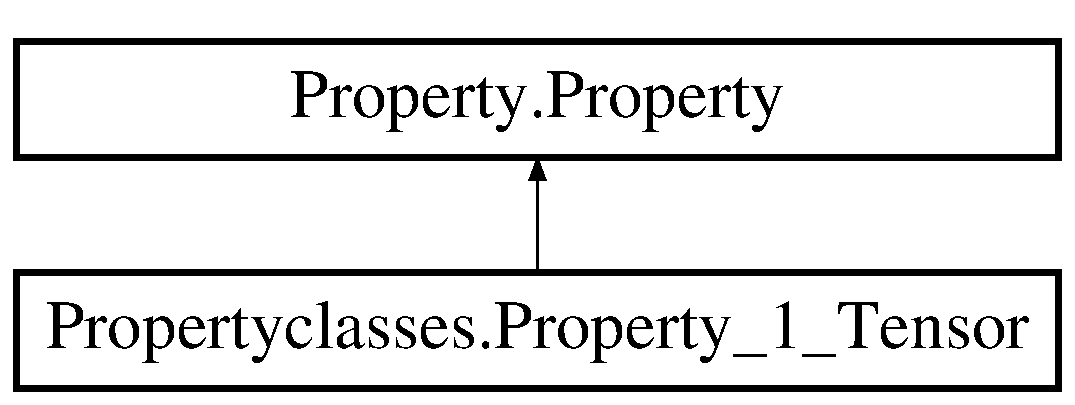
\includegraphics[height=2.000000cm]{classPropertyclasses_1_1Property__1__Tensor}
\end{center}
\end{figure}
\subsection*{Public Member Functions}
\begin{DoxyCompactItemize}
\item 
\hypertarget{classPropertyclasses_1_1Property__1__Tensor_a985c9f7efbd819f0352cee51dc444322}{def {\bfseries \+\_\+\+\_\+init\+\_\+\+\_\+}}\label{classPropertyclasses_1_1Property__1__Tensor_a985c9f7efbd819f0352cee51dc444322}

\item 
\hypertarget{classPropertyclasses_1_1Property__1__Tensor_a4b07ff551afb9b640b4de270fe127638}{def {\bfseries \+\_\+\+\_\+call\+\_\+\+\_\+}}\label{classPropertyclasses_1_1Property__1__Tensor_a4b07ff551afb9b640b4de270fe127638}

\item 
def \hyperlink{classPropertyclasses_1_1Property__1__Tensor_a8a824e2b788ed000e7ea13b2f1e2f2ce}{quartic\+\_\+precision}
\item 
\hypertarget{classPropertyclasses_1_1Property__1__Tensor_a978206dd0760d1428adc1bb8c47a8887}{def {\bfseries get\+\_\+preproperty}}\label{classPropertyclasses_1_1Property__1__Tensor_a978206dd0760d1428adc1bb8c47a8887}

\item 
\hypertarget{classPropertyclasses_1_1Property__1__Tensor_af11e9ed0dcad3c6216972ee31f04e28e}{def {\bfseries get\+\_\+prop\+\_\+grad}}\label{classPropertyclasses_1_1Property__1__Tensor_af11e9ed0dcad3c6216972ee31f04e28e}

\item 
\hypertarget{classPropertyclasses_1_1Property__1__Tensor_a975bb7a499b32983577c30aa37cc7356}{def {\bfseries get\+\_\+uncorrected\+\_\+property}}\label{classPropertyclasses_1_1Property__1__Tensor_a975bb7a499b32983577c30aa37cc7356}

\end{DoxyCompactItemize}
\subsection*{Public Attributes}
\begin{DoxyCompactItemize}
\item 
\hypertarget{classPropertyclasses_1_1Property__1__Tensor_a0bc12d39b33acba6f0ec4e7aea287697}{{\bfseries molecule}}\label{classPropertyclasses_1_1Property__1__Tensor_a0bc12d39b33acba6f0ec4e7aea287697}

\item 
\hypertarget{classPropertyclasses_1_1Property__1__Tensor_a48991d57a29bafe8c36992bddaf37ca4}{{\bfseries property\+\_\+name}}\label{classPropertyclasses_1_1Property__1__Tensor_a48991d57a29bafe8c36992bddaf37ca4}

\item 
\hypertarget{classPropertyclasses_1_1Property__1__Tensor_a1c8505bcbb89583861d52225240dbb38}{{\bfseries freq}}\label{classPropertyclasses_1_1Property__1__Tensor_a1c8505bcbb89583861d52225240dbb38}

\item 
\hypertarget{classPropertyclasses_1_1Property__1__Tensor_aaf0de1a5088ea0b5ba1af5df4f66ce3d}{{\bfseries uncorrected\+\_\+property}}\label{classPropertyclasses_1_1Property__1__Tensor_aaf0de1a5088ea0b5ba1af5df4f66ce3d}

\item 
\hypertarget{classPropertyclasses_1_1Property__1__Tensor_a9802d9fb26453b4e51cf140f0d42abb6}{{\bfseries correction\+\_\+property}}\label{classPropertyclasses_1_1Property__1__Tensor_a9802d9fb26453b4e51cf140f0d42abb6}

\item 
\hypertarget{classPropertyclasses_1_1Property__1__Tensor_a8b0ca35890e19306109e0ec99c66e6b2}{{\bfseries corrected\+\_\+property}}\label{classPropertyclasses_1_1Property__1__Tensor_a8b0ca35890e19306109e0ec99c66e6b2}

\end{DoxyCompactItemize}


\subsection{Detailed Description}
\begin{DoxyVerb}" Calculates the corrections to the dipole moment
uncorrected_property: The uncorrected dipole moment
n_nm: The number of normal modes of the molecule
pre_property: The second derivative of the dipole moment
return: The corrections to the dipole moment, the corrected dipole 
moment as np.arrays\end{DoxyVerb}
 

\subsection{Member Function Documentation}
\hypertarget{classPropertyclasses_1_1Property__1__Tensor_a8a824e2b788ed000e7ea13b2f1e2f2ce}{\index{Propertyclasses\+::\+Property\+\_\+1\+\_\+\+Tensor@{Propertyclasses\+::\+Property\+\_\+1\+\_\+\+Tensor}!quartic\+\_\+precision@{quartic\+\_\+precision}}
\index{quartic\+\_\+precision@{quartic\+\_\+precision}!Propertyclasses\+::\+Property\+\_\+1\+\_\+\+Tensor@{Propertyclasses\+::\+Property\+\_\+1\+\_\+\+Tensor}}
\subsubsection[{quartic\+\_\+precision}]{\setlength{\rightskip}{0pt plus 5cm}def Propertyclasses.\+Property\+\_\+1\+\_\+\+Tensor.\+quartic\+\_\+precision (
\begin{DoxyParamCaption}
\item[{}]{self, }
\item[{}]{prop\+\_\+deriv, }
\item[{}]{qff\+\_\+norm}
\end{DoxyParamCaption}
)}}\label{classPropertyclasses_1_1Property__1__Tensor_a8a824e2b788ed000e7ea13b2f1e2f2ce}
\begin{DoxyVerb}" Calculates the corrections to the dipole moment
uncorrected_property: The uncorrected dipole moment
pre_property: The second derivative of the dipole moment
return: The corrections to the dipole moment, the corrected dipole 
moment as np.arrays correcting to a second order perurbation 
of the wavefunction\end{DoxyVerb}
 

The documentation for this class was generated from the following file\+:\begin{DoxyCompactItemize}
\item 
Propertyclasses.\+py\end{DoxyCompactItemize}

\hypertarget{classPropertyclasses_1_1Property__2__Tensor}{\section{Propertyclasses.\+Property\+\_\+2\+\_\+\+Tensor Class Reference}
\label{classPropertyclasses_1_1Property__2__Tensor}\index{Propertyclasses.\+Property\+\_\+2\+\_\+\+Tensor@{Propertyclasses.\+Property\+\_\+2\+\_\+\+Tensor}}
}
Inheritance diagram for Propertyclasses.\+Property\+\_\+2\+\_\+\+Tensor\+:\begin{figure}[H]
\begin{center}
\leavevmode
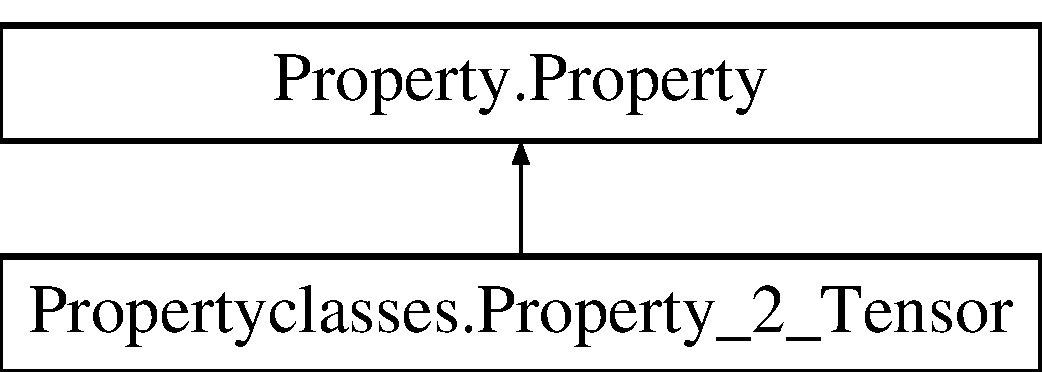
\includegraphics[height=2.000000cm]{classPropertyclasses_1_1Property__2__Tensor}
\end{center}
\end{figure}
\subsection*{Public Member Functions}
\begin{DoxyCompactItemize}
\item 
\hypertarget{classPropertyclasses_1_1Property__2__Tensor_af30d139fb36dd3f01e1751d114725e9b}{def {\bfseries \+\_\+\+\_\+init\+\_\+\+\_\+}}\label{classPropertyclasses_1_1Property__2__Tensor_af30d139fb36dd3f01e1751d114725e9b}

\item 
def \hyperlink{classPropertyclasses_1_1Property__2__Tensor_aef41af532b842a4fc2934b59e32a9b84}{\+\_\+\+\_\+call\+\_\+\+\_\+}
\item 
def \hyperlink{classPropertyclasses_1_1Property__2__Tensor_a10ce8d9ff17db524b67c598bb819c736}{quartic\+\_\+precision}
\item 
\hypertarget{classPropertyclasses_1_1Property__2__Tensor_a280a26f97a795439c8f6ea3653f4184c}{def {\bfseries get\+\_\+preproperty}}\label{classPropertyclasses_1_1Property__2__Tensor_a280a26f97a795439c8f6ea3653f4184c}

\item 
\hypertarget{classPropertyclasses_1_1Property__2__Tensor_a06b01f2819e58ebd13c9e428d846b016}{def {\bfseries get\+\_\+uncorrected\+\_\+property}}\label{classPropertyclasses_1_1Property__2__Tensor_a06b01f2819e58ebd13c9e428d846b016}

\end{DoxyCompactItemize}
\subsection*{Public Attributes}
\begin{DoxyCompactItemize}
\item 
\hypertarget{classPropertyclasses_1_1Property__2__Tensor_a614edb7a5b3f1bd7a79a70f3d3488466}{{\bfseries molecule}}\label{classPropertyclasses_1_1Property__2__Tensor_a614edb7a5b3f1bd7a79a70f3d3488466}

\item 
\hypertarget{classPropertyclasses_1_1Property__2__Tensor_afc6beeb403bffebdb699ac8359a5db8f}{{\bfseries property\+\_\+name}}\label{classPropertyclasses_1_1Property__2__Tensor_afc6beeb403bffebdb699ac8359a5db8f}

\item 
\hypertarget{classPropertyclasses_1_1Property__2__Tensor_adface3ec7178a28b985d2a9c367caca8}{{\bfseries name\+\_\+dic}}\label{classPropertyclasses_1_1Property__2__Tensor_adface3ec7178a28b985d2a9c367caca8}

\item 
\hypertarget{classPropertyclasses_1_1Property__2__Tensor_a13d5f472b33791cc18a72544fb1c8294}{{\bfseries read\+\_\+dic}}\label{classPropertyclasses_1_1Property__2__Tensor_a13d5f472b33791cc18a72544fb1c8294}

\item 
\hypertarget{classPropertyclasses_1_1Property__2__Tensor_a70863570a395baf1488f5ece05627db3}{{\bfseries read\+\_\+\+D\+A\+L\+T\+O\+N\+\_\+dic}}\label{classPropertyclasses_1_1Property__2__Tensor_a70863570a395baf1488f5ece05627db3}

\item 
\hypertarget{classPropertyclasses_1_1Property__2__Tensor_a34047db804f88e469081a58c09135cdb}{{\bfseries uncorrected\+\_\+property}}\label{classPropertyclasses_1_1Property__2__Tensor_a34047db804f88e469081a58c09135cdb}

\item 
\hypertarget{classPropertyclasses_1_1Property__2__Tensor_ab96a2fa4733028c6de7cf3d4c9651bbb}{{\bfseries uncorrected\+\_\+property1}}\label{classPropertyclasses_1_1Property__2__Tensor_ab96a2fa4733028c6de7cf3d4c9651bbb}

\item 
\hypertarget{classPropertyclasses_1_1Property__2__Tensor_ae436f0ad525c287bc646d9bb1d5cb27f}{{\bfseries uncorrected\+\_\+property2}}\label{classPropertyclasses_1_1Property__2__Tensor_ae436f0ad525c287bc646d9bb1d5cb27f}

\item 
\hypertarget{classPropertyclasses_1_1Property__2__Tensor_a4eea8b6820b34b7756b67e3564da01b0}{{\bfseries uncorrected\+\_\+property3}}\label{classPropertyclasses_1_1Property__2__Tensor_a4eea8b6820b34b7756b67e3564da01b0}

\item 
\hypertarget{classPropertyclasses_1_1Property__2__Tensor_a834fdc6bac8f03ed50241e6470dc0a84}{{\bfseries correction\+\_\+property1}}\label{classPropertyclasses_1_1Property__2__Tensor_a834fdc6bac8f03ed50241e6470dc0a84}

\item 
\hypertarget{classPropertyclasses_1_1Property__2__Tensor_a67eebc830ac19cb77552fba10a7a0fc5}{{\bfseries corrected\+\_\+property1}}\label{classPropertyclasses_1_1Property__2__Tensor_a67eebc830ac19cb77552fba10a7a0fc5}

\item 
\hypertarget{classPropertyclasses_1_1Property__2__Tensor_ac485692d5323ee1a21b44116458e6b30}{{\bfseries correction\+\_\+property2}}\label{classPropertyclasses_1_1Property__2__Tensor_ac485692d5323ee1a21b44116458e6b30}

\item 
\hypertarget{classPropertyclasses_1_1Property__2__Tensor_a0c271e5437e2a99e4a390250b17bd24f}{{\bfseries corrected\+\_\+property2}}\label{classPropertyclasses_1_1Property__2__Tensor_a0c271e5437e2a99e4a390250b17bd24f}

\item 
\hypertarget{classPropertyclasses_1_1Property__2__Tensor_aec27962dc377da9c0fee43eb3c4853d3}{{\bfseries correction\+\_\+property3}}\label{classPropertyclasses_1_1Property__2__Tensor_aec27962dc377da9c0fee43eb3c4853d3}

\item 
\hypertarget{classPropertyclasses_1_1Property__2__Tensor_ae183e92e6a5fd23086984942cffc7d4e}{{\bfseries corrected\+\_\+property3}}\label{classPropertyclasses_1_1Property__2__Tensor_ae183e92e6a5fd23086984942cffc7d4e}

\item 
\hypertarget{classPropertyclasses_1_1Property__2__Tensor_ae14493b248d39c44807033af76b2dd56}{{\bfseries correction\+\_\+property}}\label{classPropertyclasses_1_1Property__2__Tensor_ae14493b248d39c44807033af76b2dd56}

\item 
\hypertarget{classPropertyclasses_1_1Property__2__Tensor_a1fb3a921d8f41ce481fd91e9dd581fda}{{\bfseries corrected\+\_\+property}}\label{classPropertyclasses_1_1Property__2__Tensor_a1fb3a921d8f41ce481fd91e9dd581fda}

\item 
\hypertarget{classPropertyclasses_1_1Property__2__Tensor_a3c42ea53dac647e3b1082f1015cd331b}{{\bfseries freq}}\label{classPropertyclasses_1_1Property__2__Tensor_a3c42ea53dac647e3b1082f1015cd331b}

\end{DoxyCompactItemize}


\subsection{Detailed Description}
\begin{DoxyVerb}" Calculates the corrections to the g-factors, nuclear spin-rotations,
,molecular quadropole moments, and spin-spin couplings
uncorrected_property: The uncorrected property
n_nm: The number of normal modes of the molecule
pre_property: The second derivative of the property
return: The corrections to the property, the corrected property 
as np.arrays\end{DoxyVerb}
 

\subsection{Member Function Documentation}
\hypertarget{classPropertyclasses_1_1Property__2__Tensor_aef41af532b842a4fc2934b59e32a9b84}{\index{Propertyclasses\+::\+Property\+\_\+2\+\_\+\+Tensor@{Propertyclasses\+::\+Property\+\_\+2\+\_\+\+Tensor}!\+\_\+\+\_\+call\+\_\+\+\_\+@{\+\_\+\+\_\+call\+\_\+\+\_\+}}
\index{\+\_\+\+\_\+call\+\_\+\+\_\+@{\+\_\+\+\_\+call\+\_\+\+\_\+}!Propertyclasses\+::\+Property\+\_\+2\+\_\+\+Tensor@{Propertyclasses\+::\+Property\+\_\+2\+\_\+\+Tensor}}
\subsubsection[{\+\_\+\+\_\+call\+\_\+\+\_\+}]{\setlength{\rightskip}{0pt plus 5cm}def Propertyclasses.\+Property\+\_\+2\+\_\+\+Tensor.\+\_\+\+\_\+call\+\_\+\+\_\+ (
\begin{DoxyParamCaption}
\item[{}]{self}
\end{DoxyParamCaption}
)}}\label{classPropertyclasses_1_1Property__2__Tensor_aef41af532b842a4fc2934b59e32a9b84}
\begin{DoxyVerb}Calculated the vibrationally averaged corrections for first 
tensor properties. These properties are: magnetizabilities, 
rotational g-factor, molecular quadropole moments, and indirect 
spin-spin coupling, these corrections are then added to the uncorrected
propery
property_type: The name of the first tensor property, used when
       writing to file
pre_property: The second derivative of the property
Uncorrected property: The property before the corrections
nm: Number of normal modes for of the molecule
eig: The non-zero eigenvalues of the molecules hessian
returns: The corrections to the property, the corrected property as
 np.arrays
\end{DoxyVerb}
 \hypertarget{classPropertyclasses_1_1Property__2__Tensor_a10ce8d9ff17db524b67c598bb819c736}{\index{Propertyclasses\+::\+Property\+\_\+2\+\_\+\+Tensor@{Propertyclasses\+::\+Property\+\_\+2\+\_\+\+Tensor}!quartic\+\_\+precision@{quartic\+\_\+precision}}
\index{quartic\+\_\+precision@{quartic\+\_\+precision}!Propertyclasses\+::\+Property\+\_\+2\+\_\+\+Tensor@{Propertyclasses\+::\+Property\+\_\+2\+\_\+\+Tensor}}
\subsubsection[{quartic\+\_\+precision}]{\setlength{\rightskip}{0pt plus 5cm}def Propertyclasses.\+Property\+\_\+2\+\_\+\+Tensor.\+quartic\+\_\+precision (
\begin{DoxyParamCaption}
\item[{}]{self, }
\item[{}]{prop\+\_\+deriv, }
\item[{}]{qff\+\_\+norm}
\end{DoxyParamCaption}
)}}\label{classPropertyclasses_1_1Property__2__Tensor_a10ce8d9ff17db524b67c598bb819c736}
\begin{DoxyVerb}" Calculates the corrections to the dipole moment
uncorrected_property: The uncorrected dipole moment
pre_property: The second derivative of the dipole moment
return: The corrections to the dipole moment, the corrected dipole 
moment as np.arrays correcting to a second order perurbation 
of the wavefunction\end{DoxyVerb}
 

The documentation for this class was generated from the following file\+:\begin{DoxyCompactItemize}
\item 
Propertyclasses.\+py\end{DoxyCompactItemize}

\hypertarget{classPropertyclasses_1_1Property__3__Tensor}{\section{Propertyclasses.\+Property\+\_\+3\+\_\+\+Tensor Class Reference}
\label{classPropertyclasses_1_1Property__3__Tensor}\index{Propertyclasses.\+Property\+\_\+3\+\_\+\+Tensor@{Propertyclasses.\+Property\+\_\+3\+\_\+\+Tensor}}
}
Inheritance diagram for Propertyclasses.\+Property\+\_\+3\+\_\+\+Tensor\+:\begin{figure}[H]
\begin{center}
\leavevmode
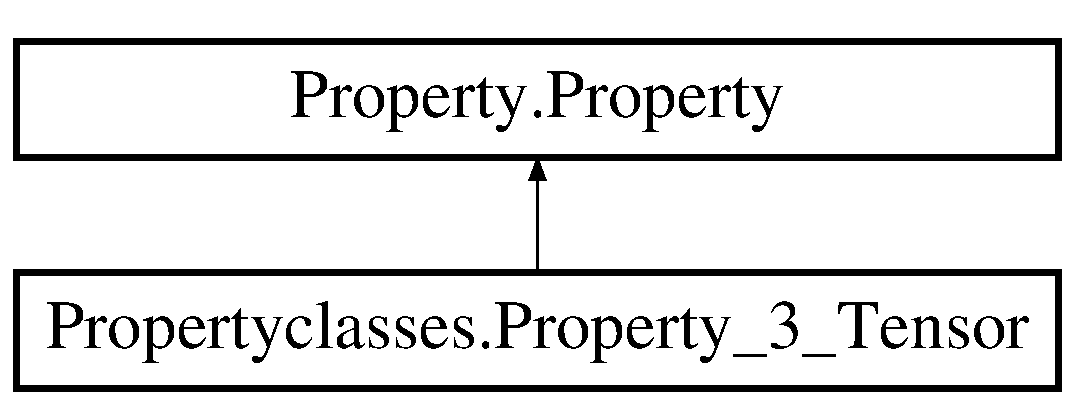
\includegraphics[height=2.000000cm]{classPropertyclasses_1_1Property__3__Tensor}
\end{center}
\end{figure}
\subsection*{Public Member Functions}
\begin{DoxyCompactItemize}
\item 
\hypertarget{classPropertyclasses_1_1Property__3__Tensor_aedf0ffda58fe2e3d50aadc103056d65c}{def {\bfseries \+\_\+\+\_\+init\+\_\+\+\_\+}}\label{classPropertyclasses_1_1Property__3__Tensor_aedf0ffda58fe2e3d50aadc103056d65c}

\item 
def \hyperlink{classPropertyclasses_1_1Property__3__Tensor_adfbcac549c9f1c741ec837421c2f9770}{\+\_\+\+\_\+call\+\_\+\+\_\+}
\item 
def \hyperlink{classPropertyclasses_1_1Property__3__Tensor_aa230b24f6eb3f2403a427d32e8cd7958}{quartic\+\_\+precision}
\item 
\hypertarget{classPropertyclasses_1_1Property__3__Tensor_a56b17dcd36be35d10668a7177e8d11b1}{def {\bfseries get\+\_\+preproperty}}\label{classPropertyclasses_1_1Property__3__Tensor_a56b17dcd36be35d10668a7177e8d11b1}

\item 
\hypertarget{classPropertyclasses_1_1Property__3__Tensor_ad43355e5980b880fbd0365284a39979a}{def {\bfseries get\+\_\+uncorrected\+\_\+property}}\label{classPropertyclasses_1_1Property__3__Tensor_ad43355e5980b880fbd0365284a39979a}

\end{DoxyCompactItemize}
\subsection*{Public Attributes}
\begin{DoxyCompactItemize}
\item 
\hypertarget{classPropertyclasses_1_1Property__3__Tensor_af6519a959ac4b3079d4a4be231f807d3}{{\bfseries molecule}}\label{classPropertyclasses_1_1Property__3__Tensor_af6519a959ac4b3079d4a4be231f807d3}

\item 
\hypertarget{classPropertyclasses_1_1Property__3__Tensor_aeeca88ff735daef742af4aa2a5c8417d}{{\bfseries property\+\_\+name}}\label{classPropertyclasses_1_1Property__3__Tensor_aeeca88ff735daef742af4aa2a5c8417d}

\item 
\hypertarget{classPropertyclasses_1_1Property__3__Tensor_a1f4da7806d0c81850d3418b44ea0bd07}{{\bfseries name\+\_\+dic}}\label{classPropertyclasses_1_1Property__3__Tensor_a1f4da7806d0c81850d3418b44ea0bd07}

\item 
\hypertarget{classPropertyclasses_1_1Property__3__Tensor_afb50d3bef512be382c54746b4e669971}{{\bfseries read\+\_\+dic}}\label{classPropertyclasses_1_1Property__3__Tensor_afb50d3bef512be382c54746b4e669971}

\item 
\hypertarget{classPropertyclasses_1_1Property__3__Tensor_acc441da9e4287120129483a780c92d31}{{\bfseries read\+\_\+\+D\+A\+L\+T\+O\+N\+\_\+dic}}\label{classPropertyclasses_1_1Property__3__Tensor_acc441da9e4287120129483a780c92d31}

\item 
\hypertarget{classPropertyclasses_1_1Property__3__Tensor_a44c0365bbf4a7d98bf97d73e5ac9509c}{{\bfseries uncorrected\+\_\+property}}\label{classPropertyclasses_1_1Property__3__Tensor_a44c0365bbf4a7d98bf97d73e5ac9509c}

\item 
\hypertarget{classPropertyclasses_1_1Property__3__Tensor_a3e8c6095e640774e344e9ec2d0fa7226}{{\bfseries correction\+\_\+property}}\label{classPropertyclasses_1_1Property__3__Tensor_a3e8c6095e640774e344e9ec2d0fa7226}

\item 
\hypertarget{classPropertyclasses_1_1Property__3__Tensor_ad9ef5ef8fabae78a0853db0191428a77}{{\bfseries corrected\+\_\+property}}\label{classPropertyclasses_1_1Property__3__Tensor_ad9ef5ef8fabae78a0853db0191428a77}

\end{DoxyCompactItemize}


\subsection{Detailed Description}
\begin{DoxyVerb}" Calculates the corrections to the nuclear shieldings,
nuclear spin correction, nuclear quadropole moment, and optical rotation 
uncorrected_property: The uncorrected property
n_nm: The number of normal modes of the molecule
pre_property: The second derivative of the property
return: The corrections to the property, the corrected property 
as np.arrays\end{DoxyVerb}
 

\subsection{Member Function Documentation}
\hypertarget{classPropertyclasses_1_1Property__3__Tensor_adfbcac549c9f1c741ec837421c2f9770}{\index{Propertyclasses\+::\+Property\+\_\+3\+\_\+\+Tensor@{Propertyclasses\+::\+Property\+\_\+3\+\_\+\+Tensor}!\+\_\+\+\_\+call\+\_\+\+\_\+@{\+\_\+\+\_\+call\+\_\+\+\_\+}}
\index{\+\_\+\+\_\+call\+\_\+\+\_\+@{\+\_\+\+\_\+call\+\_\+\+\_\+}!Propertyclasses\+::\+Property\+\_\+3\+\_\+\+Tensor@{Propertyclasses\+::\+Property\+\_\+3\+\_\+\+Tensor}}
\subsubsection[{\+\_\+\+\_\+call\+\_\+\+\_\+}]{\setlength{\rightskip}{0pt plus 5cm}def Propertyclasses.\+Property\+\_\+3\+\_\+\+Tensor.\+\_\+\+\_\+call\+\_\+\+\_\+ (
\begin{DoxyParamCaption}
\item[{}]{self}
\end{DoxyParamCaption}
)}}\label{classPropertyclasses_1_1Property__3__Tensor_adfbcac549c9f1c741ec837421c2f9770}
\begin{DoxyVerb}Calculated the vibrationally averaged corrections for first 
tensor properties. These properties are: nuclear shieldings, nuclear 
spin -rotation correction, and nuclear quadropole moments, these 
corrections are then added to the uncorrected propery

property_type: The name of the first tensor property, used when
       writing to file
pre_property: The second derivative of the property
Uncorrected property: The property before the corrections
nm: Number of normal modes for of the molecule
eig: The non-zero eigenvalues of the molecules hessian
n_atoms: The number of atoms constituting the molecule as an int
returns: The corrections to the property, the corrected property as 
 np.arrays\end{DoxyVerb}
 \hypertarget{classPropertyclasses_1_1Property__3__Tensor_aa230b24f6eb3f2403a427d32e8cd7958}{\index{Propertyclasses\+::\+Property\+\_\+3\+\_\+\+Tensor@{Propertyclasses\+::\+Property\+\_\+3\+\_\+\+Tensor}!quartic\+\_\+precision@{quartic\+\_\+precision}}
\index{quartic\+\_\+precision@{quartic\+\_\+precision}!Propertyclasses\+::\+Property\+\_\+3\+\_\+\+Tensor@{Propertyclasses\+::\+Property\+\_\+3\+\_\+\+Tensor}}
\subsubsection[{quartic\+\_\+precision}]{\setlength{\rightskip}{0pt plus 5cm}def Propertyclasses.\+Property\+\_\+3\+\_\+\+Tensor.\+quartic\+\_\+precision (
\begin{DoxyParamCaption}
{}
\end{DoxyParamCaption}
)}}\label{classPropertyclasses_1_1Property__3__Tensor_aa230b24f6eb3f2403a427d32e8cd7958}
\begin{DoxyVerb}" Calculates the corrections to the dipole moment
uncorrected_property: The uncorrected dipole moment
pre_property: The second derivative of the dipole moment
return: The corrections to the dipole moment, the corrected dipole 
moment as np.arrays correcting to a second order perurbation 
of the wavefunction\end{DoxyVerb}
 

The documentation for this class was generated from the following file\+:\begin{DoxyCompactItemize}
\item 
Propertyclasses.\+py\end{DoxyCompactItemize}

\hypertarget{classchiral__tester_1_1read__hessian__test}{\section{chiral\+\_\+tester.\+read\+\_\+hessian\+\_\+test Class Reference}
\label{classchiral__tester_1_1read__hessian__test}\index{chiral\+\_\+tester.\+read\+\_\+hessian\+\_\+test@{chiral\+\_\+tester.\+read\+\_\+hessian\+\_\+test}}
}
Inheritance diagram for chiral\+\_\+tester.\+read\+\_\+hessian\+\_\+test\+:\begin{figure}[H]
\begin{center}
\leavevmode
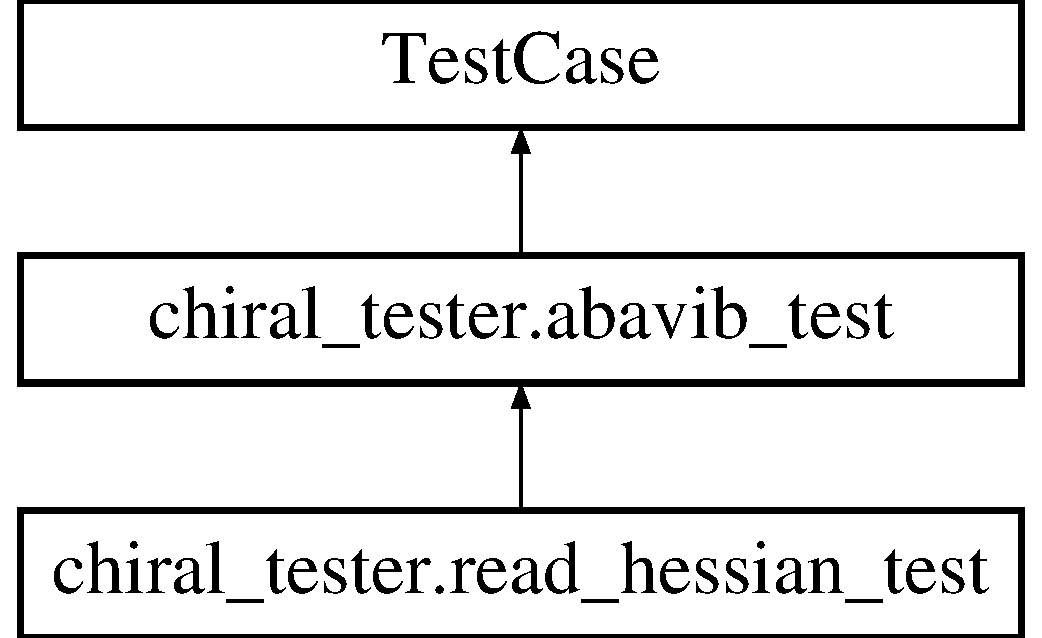
\includegraphics[height=3.000000cm]{classchiral__tester_1_1read__hessian__test}
\end{center}
\end{figure}
\subsection*{Public Member Functions}
\begin{DoxyCompactItemize}
\item 
\hypertarget{classchiral__tester_1_1read__hessian__test_a209352cb6d8ff61c1b974c8c61ea1448}{def {\bfseries test\+\_\+hessian\+\_\+values}}\label{classchiral__tester_1_1read__hessian__test_a209352cb6d8ff61c1b974c8c61ea1448}

\item 
\hypertarget{classchiral__tester_1_1read__hessian__test_a4ee8127bdcca475c42eb8e209e3601a6}{def {\bfseries test\+\_\+hessian\+\_\+dimensions}}\label{classchiral__tester_1_1read__hessian__test_a4ee8127bdcca475c42eb8e209e3601a6}

\end{DoxyCompactItemize}
\subsection*{Public Attributes}
\begin{DoxyCompactItemize}
\item 
\hypertarget{classchiral__tester_1_1read__hessian__test_a4e0900d43d3cd8b6e02233b350b145fd}{{\bfseries molecule}}\label{classchiral__tester_1_1read__hessian__test_a4e0900d43d3cd8b6e02233b350b145fd}

\item 
\hypertarget{classchiral__tester_1_1read__hessian__test_a8a2cf17bff86d2f232645b635998d405}{{\bfseries hessian}}\label{classchiral__tester_1_1read__hessian__test_a8a2cf17bff86d2f232645b635998d405}

\end{DoxyCompactItemize}
\subsection*{Additional Inherited Members}


The documentation for this class was generated from the following file\+:\begin{DoxyCompactItemize}
\item 
chiral\+\_\+tester.\+py\end{DoxyCompactItemize}

\hypertarget{classabavib__unittester_1_1read__hessian__test}{\section{abavib\+\_\+unittester.\+read\+\_\+hessian\+\_\+test Class Reference}
\label{classabavib__unittester_1_1read__hessian__test}\index{abavib\+\_\+unittester.\+read\+\_\+hessian\+\_\+test@{abavib\+\_\+unittester.\+read\+\_\+hessian\+\_\+test}}
}
Inheritance diagram for abavib\+\_\+unittester.\+read\+\_\+hessian\+\_\+test\+:\begin{figure}[H]
\begin{center}
\leavevmode
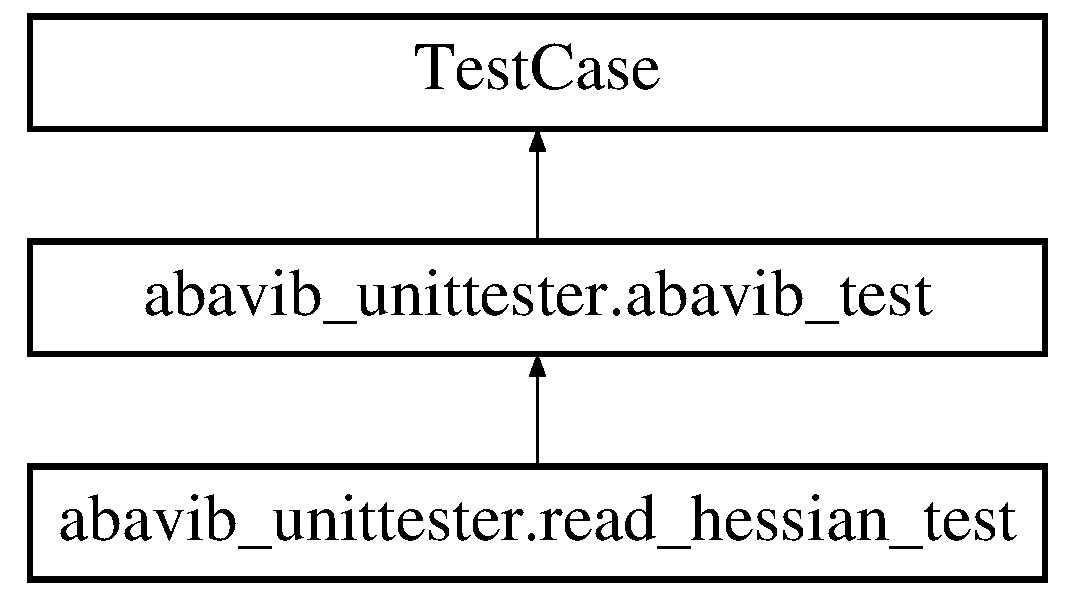
\includegraphics[height=3.000000cm]{classabavib__unittester_1_1read__hessian__test}
\end{center}
\end{figure}
\subsection*{Public Member Functions}
\begin{DoxyCompactItemize}
\item 
\hypertarget{classabavib__unittester_1_1read__hessian__test_aca294204b35ad6feb0161aae379296cc}{def {\bfseries test\+\_\+hessian\+\_\+values}}\label{classabavib__unittester_1_1read__hessian__test_aca294204b35ad6feb0161aae379296cc}

\item 
\hypertarget{classabavib__unittester_1_1read__hessian__test_adee645671ac9fc43398afb66a11d1ddf}{def {\bfseries test\+\_\+hessian\+\_\+dimensions}}\label{classabavib__unittester_1_1read__hessian__test_adee645671ac9fc43398afb66a11d1ddf}

\end{DoxyCompactItemize}
\subsection*{Public Attributes}
\begin{DoxyCompactItemize}
\item 
\hypertarget{classabavib__unittester_1_1read__hessian__test_a41f0724afcbf8189c2615251910aa684}{{\bfseries molecule}}\label{classabavib__unittester_1_1read__hessian__test_a41f0724afcbf8189c2615251910aa684}

\item 
\hypertarget{classabavib__unittester_1_1read__hessian__test_af67af78bb936974d10272d206c11c8ed}{{\bfseries hessian}}\label{classabavib__unittester_1_1read__hessian__test_af67af78bb936974d10272d206c11c8ed}

\end{DoxyCompactItemize}
\subsection*{Additional Inherited Members}


The documentation for this class was generated from the following file\+:\begin{DoxyCompactItemize}
\item 
abavib\+\_\+unittester.\+py\end{DoxyCompactItemize}

\hypertarget{classchiral__tester_1_1read__molecule__test}{\section{chiral\+\_\+tester.\+read\+\_\+molecule\+\_\+test Class Reference}
\label{classchiral__tester_1_1read__molecule__test}\index{chiral\+\_\+tester.\+read\+\_\+molecule\+\_\+test@{chiral\+\_\+tester.\+read\+\_\+molecule\+\_\+test}}
}
Inheritance diagram for chiral\+\_\+tester.\+read\+\_\+molecule\+\_\+test\+:\begin{figure}[H]
\begin{center}
\leavevmode
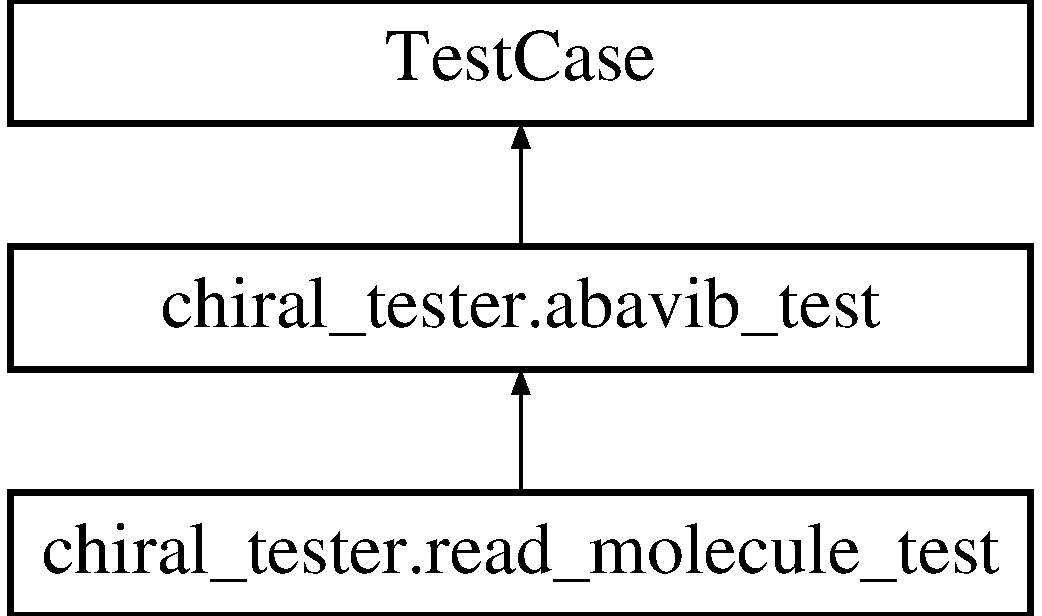
\includegraphics[height=3.000000cm]{classchiral__tester_1_1read__molecule__test}
\end{center}
\end{figure}
\subsection*{Public Member Functions}
\begin{DoxyCompactItemize}
\item 
\hypertarget{classchiral__tester_1_1read__molecule__test_ac881ffd684209c4d1bab8136b74261ed}{def {\bfseries test\+\_\+coordinates}}\label{classchiral__tester_1_1read__molecule__test_ac881ffd684209c4d1bab8136b74261ed}

\item 
\hypertarget{classchiral__tester_1_1read__molecule__test_a6b02e84c4165ca4faaa14bcdca6e2641}{def {\bfseries test\+\_\+masses}}\label{classchiral__tester_1_1read__molecule__test_a6b02e84c4165ca4faaa14bcdca6e2641}

\item 
\hypertarget{classchiral__tester_1_1read__molecule__test_ab4e464a0bb098ca742ff7036a80d1727}{def {\bfseries test\+\_\+n\+\_\+atoms}}\label{classchiral__tester_1_1read__molecule__test_ab4e464a0bb098ca742ff7036a80d1727}

\end{DoxyCompactItemize}
\subsection*{Public Attributes}
\begin{DoxyCompactItemize}
\item 
\hypertarget{classchiral__tester_1_1read__molecule__test_a527090ddc7f30f058cbbd84a830e744d}{{\bfseries molecule}}\label{classchiral__tester_1_1read__molecule__test_a527090ddc7f30f058cbbd84a830e744d}

\item 
\hypertarget{classchiral__tester_1_1read__molecule__test_a737337aaea450f8b30d15f9cd6c10c23}{{\bfseries correct\+\_\+coordinates}}\label{classchiral__tester_1_1read__molecule__test_a737337aaea450f8b30d15f9cd6c10c23}

\item 
\hypertarget{classchiral__tester_1_1read__molecule__test_a827a4cfa7aebc4f347034daade46d1ba}{{\bfseries coordinates}}\label{classchiral__tester_1_1read__molecule__test_a827a4cfa7aebc4f347034daade46d1ba}

\item 
\hypertarget{classchiral__tester_1_1read__molecule__test_ad9c2f5342740e78ee4852b16407c2649}{{\bfseries correct\+\_\+masses}}\label{classchiral__tester_1_1read__molecule__test_ad9c2f5342740e78ee4852b16407c2649}

\end{DoxyCompactItemize}
\subsection*{Additional Inherited Members}


The documentation for this class was generated from the following file\+:\begin{DoxyCompactItemize}
\item 
chiral\+\_\+tester.\+py\end{DoxyCompactItemize}

\hypertarget{classabavib__unittester_1_1read__molecule__test}{\section{abavib\+\_\+unittester.\+read\+\_\+molecule\+\_\+test Class Reference}
\label{classabavib__unittester_1_1read__molecule__test}\index{abavib\+\_\+unittester.\+read\+\_\+molecule\+\_\+test@{abavib\+\_\+unittester.\+read\+\_\+molecule\+\_\+test}}
}
Inheritance diagram for abavib\+\_\+unittester.\+read\+\_\+molecule\+\_\+test\+:\begin{figure}[H]
\begin{center}
\leavevmode
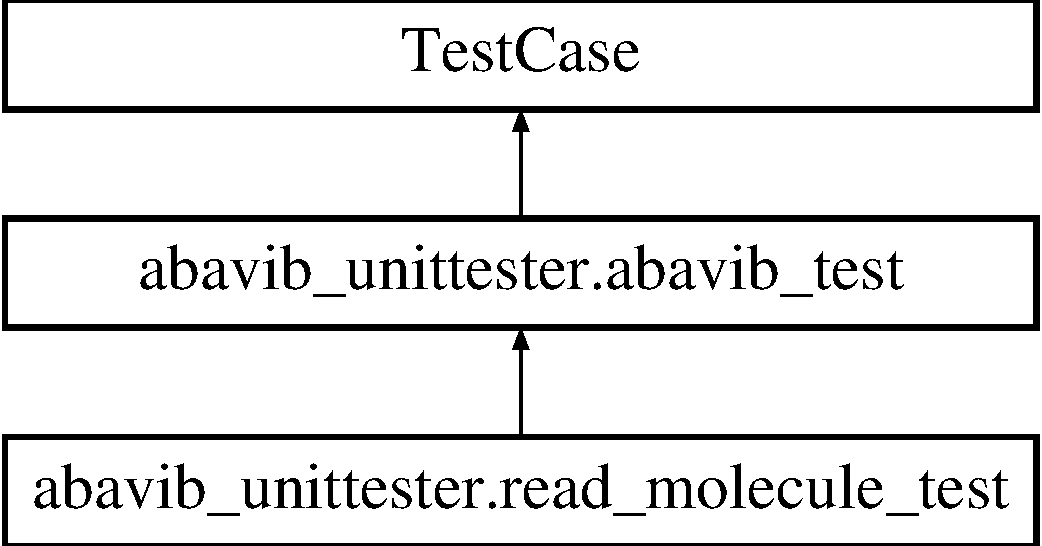
\includegraphics[height=3.000000cm]{classabavib__unittester_1_1read__molecule__test}
\end{center}
\end{figure}
\subsection*{Public Member Functions}
\begin{DoxyCompactItemize}
\item 
\hypertarget{classabavib__unittester_1_1read__molecule__test_ab2944b667d4d096a4386c89cb8a7c44a}{def {\bfseries test\+\_\+coordinates}}\label{classabavib__unittester_1_1read__molecule__test_ab2944b667d4d096a4386c89cb8a7c44a}

\item 
\hypertarget{classabavib__unittester_1_1read__molecule__test_a63546c5c77b2b10fa3ebc0efa30cc9a6}{def {\bfseries test\+\_\+masses}}\label{classabavib__unittester_1_1read__molecule__test_a63546c5c77b2b10fa3ebc0efa30cc9a6}

\item 
\hypertarget{classabavib__unittester_1_1read__molecule__test_a64f2177206444f824938a18b54fe3636}{def {\bfseries test\+\_\+num\+\_\+atoms\+\_\+list}}\label{classabavib__unittester_1_1read__molecule__test_a64f2177206444f824938a18b54fe3636}

\item 
\hypertarget{classabavib__unittester_1_1read__molecule__test_a0642a77c8a56affe42489a7c554754ba}{def {\bfseries test\+\_\+charge\+\_\+list}}\label{classabavib__unittester_1_1read__molecule__test_a0642a77c8a56affe42489a7c554754ba}

\item 
\hypertarget{classabavib__unittester_1_1read__molecule__test_a1e1c510c35f2316280baac8e6c1c3ebc}{def {\bfseries test\+\_\+n\+\_\+atoms}}\label{classabavib__unittester_1_1read__molecule__test_a1e1c510c35f2316280baac8e6c1c3ebc}

\end{DoxyCompactItemize}
\subsection*{Public Attributes}
\begin{DoxyCompactItemize}
\item 
\hypertarget{classabavib__unittester_1_1read__molecule__test_aa63a86b5182ed37df4e9c981a47aef83}{{\bfseries molecule}}\label{classabavib__unittester_1_1read__molecule__test_aa63a86b5182ed37df4e9c981a47aef83}

\item 
\hypertarget{classabavib__unittester_1_1read__molecule__test_a60cc70142230b595b961756e53cda062}{{\bfseries correct\+\_\+coordinates}}\label{classabavib__unittester_1_1read__molecule__test_a60cc70142230b595b961756e53cda062}

\item 
\hypertarget{classabavib__unittester_1_1read__molecule__test_a2303ff7a039d016a0ff8dea65c4bb39b}{{\bfseries coordinates}}\label{classabavib__unittester_1_1read__molecule__test_a2303ff7a039d016a0ff8dea65c4bb39b}

\item 
\hypertarget{classabavib__unittester_1_1read__molecule__test_ab58a35e57fc355d781fe03c4d904b6c9}{{\bfseries correct\+\_\+masses}}\label{classabavib__unittester_1_1read__molecule__test_ab58a35e57fc355d781fe03c4d904b6c9}

\end{DoxyCompactItemize}
\subsection*{Additional Inherited Members}


The documentation for this class was generated from the following file\+:\begin{DoxyCompactItemize}
\item 
abavib\+\_\+unittester.\+py\end{DoxyCompactItemize}

\hypertarget{classabavib__unittester_1_1shield__test}{\section{abavib\+\_\+unittester.\+shield\+\_\+test Class Reference}
\label{classabavib__unittester_1_1shield__test}\index{abavib\+\_\+unittester.\+shield\+\_\+test@{abavib\+\_\+unittester.\+shield\+\_\+test}}
}
Inheritance diagram for abavib\+\_\+unittester.\+shield\+\_\+test\+:\begin{figure}[H]
\begin{center}
\leavevmode
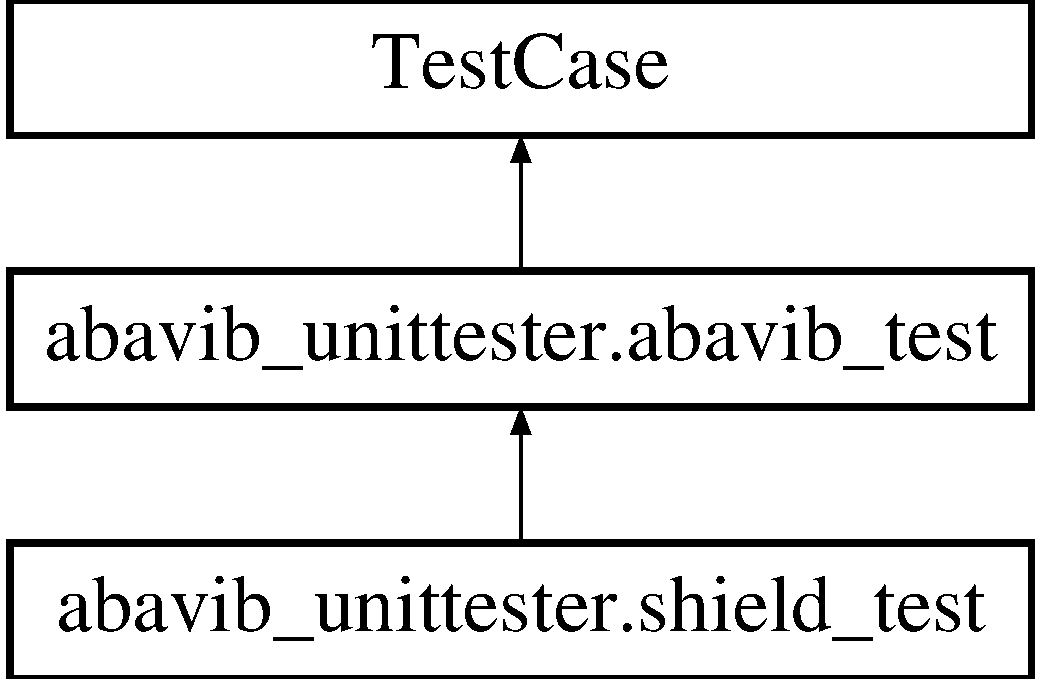
\includegraphics[height=3.000000cm]{classabavib__unittester_1_1shield__test}
\end{center}
\end{figure}
\subsection*{Public Member Functions}
\begin{DoxyCompactItemize}
\item 
\hypertarget{classabavib__unittester_1_1shield__test_a0be7b73cb7edd0d2ce164be2567f302a}{def {\bfseries set\+Up}}\label{classabavib__unittester_1_1shield__test_a0be7b73cb7edd0d2ce164be2567f302a}

\item 
\hypertarget{classabavib__unittester_1_1shield__test_ab330ebe268b30e1da3c1a19dd3eaca17}{def {\bfseries test\+\_\+shield\+\_\+corrections}}\label{classabavib__unittester_1_1shield__test_ab330ebe268b30e1da3c1a19dd3eaca17}

\item 
\hypertarget{classabavib__unittester_1_1shield__test_a782de883f3e5356f1fe465544046a5b1}{def {\bfseries test\+\_\+shield\+\_\+values}}\label{classabavib__unittester_1_1shield__test_a782de883f3e5356f1fe465544046a5b1}

\end{DoxyCompactItemize}
\subsection*{Public Attributes}
\begin{DoxyCompactItemize}
\item 
\hypertarget{classabavib__unittester_1_1shield__test_a285f92b82f7a149c484452e55fcea707}{{\bfseries prop\+\_\+type}}\label{classabavib__unittester_1_1shield__test_a285f92b82f7a149c484452e55fcea707}

\item 
\hypertarget{classabavib__unittester_1_1shield__test_a177a0753de121fd13b7b68e59526a70b}{{\bfseries corrected\+\_\+values}}\label{classabavib__unittester_1_1shield__test_a177a0753de121fd13b7b68e59526a70b}

\item 
\hypertarget{classabavib__unittester_1_1shield__test_afa8a05a4a30dfff0a7b6af258a160142}{{\bfseries shield}}\label{classabavib__unittester_1_1shield__test_afa8a05a4a30dfff0a7b6af258a160142}

\item 
\hypertarget{classabavib__unittester_1_1shield__test_aebee7b74c39b728c5516961c2bf6b3d6}{{\bfseries molecule}}\label{classabavib__unittester_1_1shield__test_aebee7b74c39b728c5516961c2bf6b3d6}

\end{DoxyCompactItemize}
\subsection*{Additional Inherited Members}


The documentation for this class was generated from the following file\+:\begin{DoxyCompactItemize}
\item 
abavib\+\_\+unittester.\+py\end{DoxyCompactItemize}

\hypertarget{classabavib__unittester_1_1spin__rotation__constants__test}{\section{abavib\+\_\+unittester.\+spin\+\_\+rotation\+\_\+constants\+\_\+test Class Reference}
\label{classabavib__unittester_1_1spin__rotation__constants__test}\index{abavib\+\_\+unittester.\+spin\+\_\+rotation\+\_\+constants\+\_\+test@{abavib\+\_\+unittester.\+spin\+\_\+rotation\+\_\+constants\+\_\+test}}
}
Inheritance diagram for abavib\+\_\+unittester.\+spin\+\_\+rotation\+\_\+constants\+\_\+test\+:\begin{figure}[H]
\begin{center}
\leavevmode
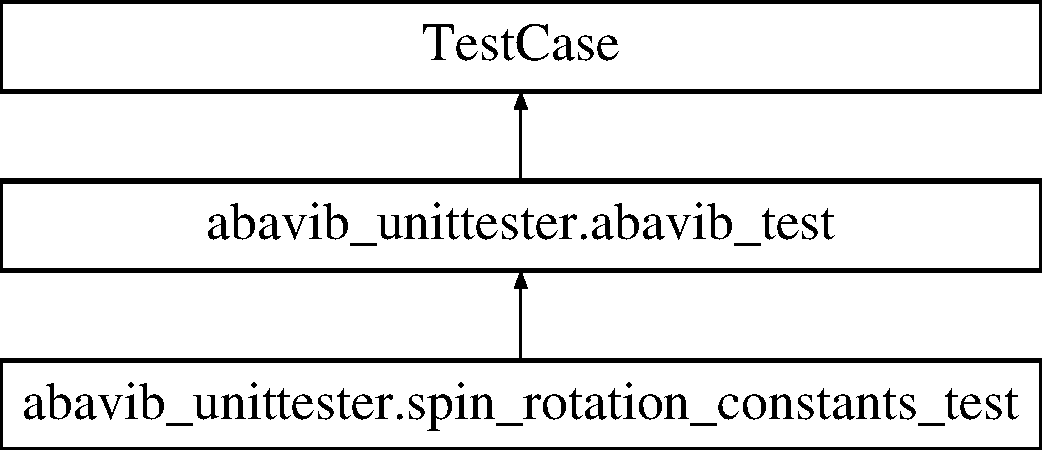
\includegraphics[height=3.000000cm]{classabavib__unittester_1_1spin__rotation__constants__test}
\end{center}
\end{figure}
\subsection*{Additional Inherited Members}


The documentation for this class was generated from the following file\+:\begin{DoxyCompactItemize}
\item 
abavib\+\_\+unittester.\+py\end{DoxyCompactItemize}

%--- End generated contents ---

% Index
\newpage
\phantomsection
\addcontentsline{toc}{chapter}{Index}
\printindex

\end{document}
